% Options for packages loaded elsewhere
\PassOptionsToPackage{unicode}{hyperref}
\PassOptionsToPackage{hyphens}{url}
%
\documentclass[
]{book}
\usepackage{amsmath,amssymb}
\usepackage{lmodern}
\usepackage{iftex}
\ifPDFTeX
  \usepackage[T1]{fontenc}
  \usepackage[utf8]{inputenc}
  \usepackage{textcomp} % provide euro and other symbols
\else % if luatex or xetex
  \usepackage{unicode-math}
  \defaultfontfeatures{Scale=MatchLowercase}
  \defaultfontfeatures[\rmfamily]{Ligatures=TeX,Scale=1}
  \setmainfont[]{NanumGothic}
\fi
% Use upquote if available, for straight quotes in verbatim environments
\IfFileExists{upquote.sty}{\usepackage{upquote}}{}
\IfFileExists{microtype.sty}{% use microtype if available
  \usepackage[]{microtype}
  \UseMicrotypeSet[protrusion]{basicmath} % disable protrusion for tt fonts
}{}
\makeatletter
\@ifundefined{KOMAClassName}{% if non-KOMA class
  \IfFileExists{parskip.sty}{%
    \usepackage{parskip}
  }{% else
    \setlength{\parindent}{0pt}
    \setlength{\parskip}{6pt plus 2pt minus 1pt}}
}{% if KOMA class
  \KOMAoptions{parskip=half}}
\makeatother
\usepackage{xcolor}
\usepackage{color}
\usepackage{fancyvrb}
\newcommand{\VerbBar}{|}
\newcommand{\VERB}{\Verb[commandchars=\\\{\}]}
\DefineVerbatimEnvironment{Highlighting}{Verbatim}{commandchars=\\\{\}}
% Add ',fontsize=\small' for more characters per line
\usepackage{framed}
\definecolor{shadecolor}{RGB}{248,248,248}
\newenvironment{Shaded}{\begin{snugshade}}{\end{snugshade}}
\newcommand{\AlertTok}[1]{\textcolor[rgb]{0.94,0.16,0.16}{#1}}
\newcommand{\AnnotationTok}[1]{\textcolor[rgb]{0.56,0.35,0.01}{\textbf{\textit{#1}}}}
\newcommand{\AttributeTok}[1]{\textcolor[rgb]{0.77,0.63,0.00}{#1}}
\newcommand{\BaseNTok}[1]{\textcolor[rgb]{0.00,0.00,0.81}{#1}}
\newcommand{\BuiltInTok}[1]{#1}
\newcommand{\CharTok}[1]{\textcolor[rgb]{0.31,0.60,0.02}{#1}}
\newcommand{\CommentTok}[1]{\textcolor[rgb]{0.56,0.35,0.01}{\textit{#1}}}
\newcommand{\CommentVarTok}[1]{\textcolor[rgb]{0.56,0.35,0.01}{\textbf{\textit{#1}}}}
\newcommand{\ConstantTok}[1]{\textcolor[rgb]{0.00,0.00,0.00}{#1}}
\newcommand{\ControlFlowTok}[1]{\textcolor[rgb]{0.13,0.29,0.53}{\textbf{#1}}}
\newcommand{\DataTypeTok}[1]{\textcolor[rgb]{0.13,0.29,0.53}{#1}}
\newcommand{\DecValTok}[1]{\textcolor[rgb]{0.00,0.00,0.81}{#1}}
\newcommand{\DocumentationTok}[1]{\textcolor[rgb]{0.56,0.35,0.01}{\textbf{\textit{#1}}}}
\newcommand{\ErrorTok}[1]{\textcolor[rgb]{0.64,0.00,0.00}{\textbf{#1}}}
\newcommand{\ExtensionTok}[1]{#1}
\newcommand{\FloatTok}[1]{\textcolor[rgb]{0.00,0.00,0.81}{#1}}
\newcommand{\FunctionTok}[1]{\textcolor[rgb]{0.00,0.00,0.00}{#1}}
\newcommand{\ImportTok}[1]{#1}
\newcommand{\InformationTok}[1]{\textcolor[rgb]{0.56,0.35,0.01}{\textbf{\textit{#1}}}}
\newcommand{\KeywordTok}[1]{\textcolor[rgb]{0.13,0.29,0.53}{\textbf{#1}}}
\newcommand{\NormalTok}[1]{#1}
\newcommand{\OperatorTok}[1]{\textcolor[rgb]{0.81,0.36,0.00}{\textbf{#1}}}
\newcommand{\OtherTok}[1]{\textcolor[rgb]{0.56,0.35,0.01}{#1}}
\newcommand{\PreprocessorTok}[1]{\textcolor[rgb]{0.56,0.35,0.01}{\textit{#1}}}
\newcommand{\RegionMarkerTok}[1]{#1}
\newcommand{\SpecialCharTok}[1]{\textcolor[rgb]{0.00,0.00,0.00}{#1}}
\newcommand{\SpecialStringTok}[1]{\textcolor[rgb]{0.31,0.60,0.02}{#1}}
\newcommand{\StringTok}[1]{\textcolor[rgb]{0.31,0.60,0.02}{#1}}
\newcommand{\VariableTok}[1]{\textcolor[rgb]{0.00,0.00,0.00}{#1}}
\newcommand{\VerbatimStringTok}[1]{\textcolor[rgb]{0.31,0.60,0.02}{#1}}
\newcommand{\WarningTok}[1]{\textcolor[rgb]{0.56,0.35,0.01}{\textbf{\textit{#1}}}}
\usepackage{longtable,booktabs,array}
\usepackage{calc} % for calculating minipage widths
% Correct order of tables after \paragraph or \subparagraph
\usepackage{etoolbox}
\makeatletter
\patchcmd\longtable{\par}{\if@noskipsec\mbox{}\fi\par}{}{}
\makeatother
% Allow footnotes in longtable head/foot
\IfFileExists{footnotehyper.sty}{\usepackage{footnotehyper}}{\usepackage{footnote}}
\makesavenoteenv{longtable}
\usepackage{graphicx}
\makeatletter
\def\maxwidth{\ifdim\Gin@nat@width>\linewidth\linewidth\else\Gin@nat@width\fi}
\def\maxheight{\ifdim\Gin@nat@height>\textheight\textheight\else\Gin@nat@height\fi}
\makeatother
% Scale images if necessary, so that they will not overflow the page
% margins by default, and it is still possible to overwrite the defaults
% using explicit options in \includegraphics[width, height, ...]{}
\setkeys{Gin}{width=\maxwidth,height=\maxheight,keepaspectratio}
% Set default figure placement to htbp
\makeatletter
\def\fps@figure{htbp}
\makeatother
\setlength{\emergencystretch}{3em} % prevent overfull lines
\providecommand{\tightlist}{%
  \setlength{\itemsep}{0pt}\setlength{\parskip}{0pt}}
\setcounter{secnumdepth}{5}
\usepackage{booktabs}
\ifLuaTeX
  \usepackage{selnolig}  % disable illegal ligatures
\fi
\usepackage[]{natbib}
\bibliographystyle{apalike}
\IfFileExists{bookmark.sty}{\usepackage{bookmark}}{\usepackage{hyperref}}
\IfFileExists{xurl.sty}{\usepackage{xurl}}{} % add URL line breaks if available
\urlstyle{same} % disable monospaced font for URLs
\hypersetup{
  pdftitle={2022년 한국생명공학연구원 연구데이터 분석과정 R},
  pdfauthor={합성생물학전문연구소 김하성},
  hidelinks,
  pdfcreator={LaTeX via pandoc}}

\title{2022년 한국생명공학연구원 연구데이터 분석과정 R}
\author{합성생물학전문연구소 김하성}
\date{2022-06-08}

\begin{document}
\maketitle

{
\setcounter{tocdepth}{1}
\tableofcontents
}
\hypertarget{introduction}{%
\chapter{Introduction}\label{introduction}}

\hypertarget{Information}{%
\section{강의 개요}\label{Information}}

\begin{itemize}
\tightlist
\item
  목표: 생물 데이터 분석을 위한 R 사용법과 (Rstudio, Tidyverse, Bioconductor 포함) 프로그래밍 기술을 습득함
\item
  장소: 코빅 3층 전산교육장(1304호)
\item
  강사: 한국생명공학연구원 합성생물학전문연구단 김하성
\item
  연락처: 042-860-4372, \href{mailto:haseong@kribb.re.kr}{\nolinkurl{haseong@kribb.re.kr}}
\item
  강의자료: \url{https://greendaygh.github.io/kribbr2022/}
\end{itemize}

\hypertarget{Schedule}{%
\section{강의 계획}\label{Schedule}}

\begin{enumerate}
\def\labelenumi{\arabic{enumi}.}
\tightlist
\item
  R 사용법 및 데이터 분석 기초 5.19(목), 5.26(목)
\item
  R/Tidyverse 데이터 분석 중급 6.9(목), 6.16(목)
\item
  R/Tidyverse 활용 데이터 가시화 7.7(목), 7.14(목)
\item
  R/Bioconductor 활용한 바이오데이터 분석 기초 8.4(목), 8.11(목)
\item
  R/Bioconductor 활용한 NGS 데이터 분석 기초 9.1(목), 9.15(목)
\item
  R/Bioconductor 활용한 NGS 데이터 분석 및 Workflow 10.6(목), 10.13(목)
\end{enumerate}

\hypertarget{References}{%
\section{참고 자료}\label{References}}

\begin{itemize}
\tightlist
\item
  \href{https://www.r-project.org/}{R 홈페이지}
\item
  \href{https://www.rstudio.com/}{Rstudio 홈페이지}
\item
  \href{https://www.bioconductor.org/}{Bioconductor}
\item
  \href{https://cran.r-project.org/manuals.html}{R 기본 문서들}
\item
  \href{https://bookdown.org/}{R ebooks}
\item
  \href{https://www.rstudio.com/resources/cheatsheets/}{Cheat Sheets}
\item
  \href{https://resources.rstudio.com/}{RStudio Webinars}
\item
  \href{http://shiny.rstudio.com/tutorial/}{Shiny}
\item
  \href{https://github.com/hadley}{Hadley github}
\item
  \href{https://r4ds.had.co.nz}{R for Data Science}
\item
  Using R for Introductory Statistics by John Verzani

  \begin{itemize}
  \tightlist
  \item
    Free version of \href{https://cran.r-project.org/doc/contrib/Verzani-SimpleR.pdf}{1st Edition}
  \item
    \href{https://www.crcpress.com/Using-R-for-Introductory-Statistics-Second-Edition/Verzani/p/book/9781466590731}{Second edition}
  \end{itemize}
\item
  \href{http://2.droppdf.com/files/5aTvl/bioinformatics-data-skills.pdf}{Bioinformatics Data Skills} by Vince Buffalo
\item
  \href{http://www.academia.dk/BiologiskAntropologi/Epidemiologi/PDF/Introductory_Statistics_with_R__2nd_ed.pdf}{Introductory Statistics with R} by Dalgaard
\item
  일반통계학 (영지문화사, 김우철 외)
\end{itemize}

\hypertarget{rrstudio-basics}{%
\chapter{R/Rstudio basics}\label{rrstudio-basics}}

\hypertarget{what-is-r-rstudio}{%
\section{What is R / Rstudio}\label{what-is-r-rstudio}}


\includegraphics[width=1.04167in,height=\textheight]{images/01/r.jpg}

R은 통계나 생물통계, 유전학을 연구하는 사람들 사이에서 널리 사용되는 오픈소스 프로그래밍 언어 입니다. Bell Lab에서 개발한 S 언어에서 유래했으며 많은 라이브러리 (다른 사람들이 만들어 놓은 코드)가 있어서 쉽게 가져다 사용할 수 있습니다. R은 복잡한 수식이나 통계 알고리즘을 간단히 구현하고 사용할 수 있으며 C, C++, Python 등 다른 언어들과의 병행 사용도 가능합니다. R은 IEEE에서 조사하는 Top programming languages에서 2018년 7위, 2019년 5위, 2020년 6위, 2021년 7위로 꾸준히 높은 사용자를 확보하며 빅데이터, AI 시대의 주요한 프로그래밍 언어로 사용되고 있습니다.

\begin{figure}
\centering
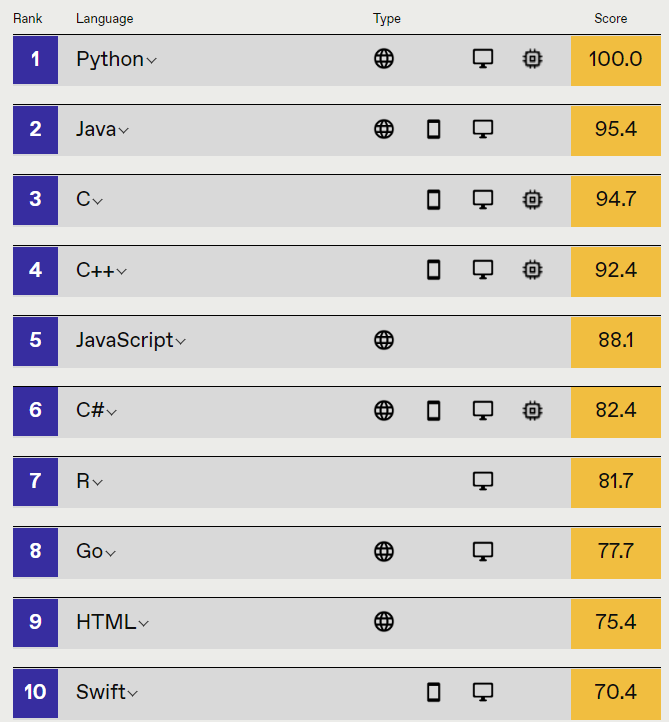
\includegraphics[width=2.60417in,height=\textheight]{images/01/toplanguage2021.png}
\caption{\url{https://spectrum.ieee.org/top-programming-languages/}}
\end{figure}

R은 데이터를 통계분석에 널리 사용되는데 이는 데이터를 눈으로 확인하기 위한 visualization 이나 벡터 연산 등의 강력한 기능 때문에 점점 더 많은 사람들이 사용하고 있습니다. 기존에는 속도나 확장성이 다른 언어들에 비해 단점으로 지적되었으나 R 언어의 계속적인 개발과 업데이트로 이러한 단점들이 빠르게 보완되고 있습니다. R 사용을 위해서는 R 언어의 코어 프로그램을 먼저 설치하고 그 다음 R 언어용 IDE(Integrated Development Environment)인 RStudio 설치가 필요합니다.


\includegraphics[width=1.5625in,height=\textheight]{images/01/rstudio.png}

Rstudio는 R 언어를 위한 오픈소스 기반 통합개발환경(IDE)으로 R 프로그래밍을 위한 편리한 기능들을 제공해 줍니다. R언어가 주목을 받고 두터운 사용자 층을 확보할 수 있게된 핵심 동력이 Rstudio 입니다. 자체적으로 최고수준의 오픈소스 개발팀이 있으며 \texttt{tidyverse}, `\texttt{,}shiny` 등의 데이터 분석 관련 주요 패키지를 개발하였고 정기적으로 conference 개최를 하면서 기술 보급의 핵심 역할을 하고 있습니다.

\begin{figure}
\centering
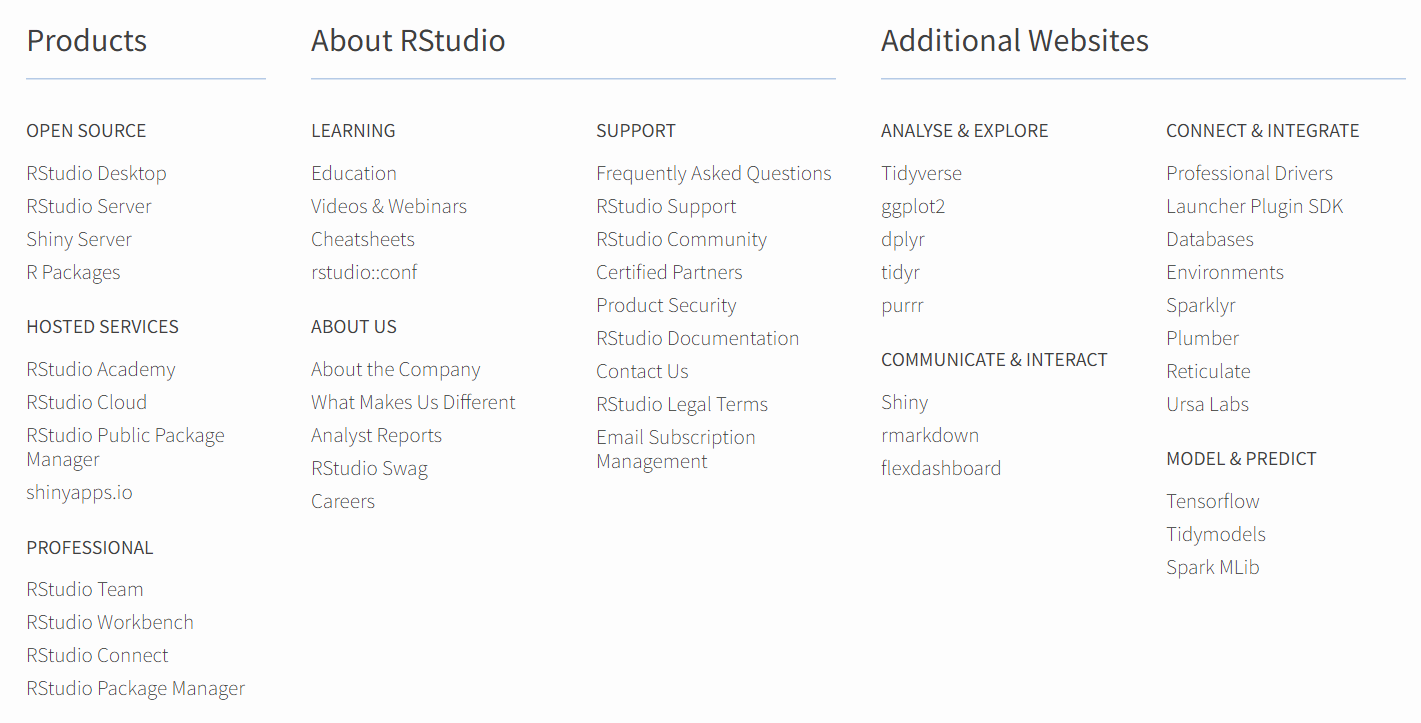
\includegraphics[width=5.72917in,height=\textheight]{images/01/rstudiobottom.png}
\caption{\url{https://www.rstudio.com/}}
\end{figure}

\hypertarget{r-rstudio-installation}{%
\section{R / Rstudio Installation}\label{r-rstudio-installation}}

\hypertarget{r-uxc124uxce58}{%
\subsection{R 설치}\label{r-uxc124uxce58}}

\begin{itemize}
\tightlist
\item
  R 사이트에 접속 후 (\url{https://www.r-project.org/}) 좌측 메뉴 상단에 위치한 CRAN 클릭.
\item
  미러 사이트 목록에서 Korea의 아무 사이트나 들어감
\item
  Download R for Windows를 클릭 후 base 링크 들어가서
\item
  Download R x.x.x for Windows 링크 클릭으로 실행 프로그램 다운로드
\item
  로컬 컴퓨터에 Download 된 R-x.x.x-win.exe 를 실행 (2022.5 현재 R 버전은 4.2.0).
\item
  설치 프로그램의 지시에 따라 R 언어 소프트웨어 설치를 완료
\end{itemize}

\hypertarget{rstudio-uxc124uxce58}{%
\subsection{Rstudio 설치}\label{rstudio-uxc124uxce58}}

\begin{itemize}
\tightlist
\item
  사이트에 접속 (\url{https://www.rstudio.com/}), 상단의 Products \textgreater{} RStudio 클릭
\item
  RStudio Desktop 선택
\item
  Download RStudio Desktop 클릭
\item
  RStudio Desktop Free 버전의 Download를 선택하고
\item
  Download RStudio for Windows 클릭, 다운로드
\item
  로컬 컴퓨터에 다운로드된 RStudio-x.x.x.exe 실행 (2022.5 현재 RStudio Desktop 2022.02.2+485)
\item
  설치 가이드에 따라 설치 완료
\end{itemize}

\hypertarget{rstudio-interface}{%
\section{Rstudio interface}\label{rstudio-interface}}

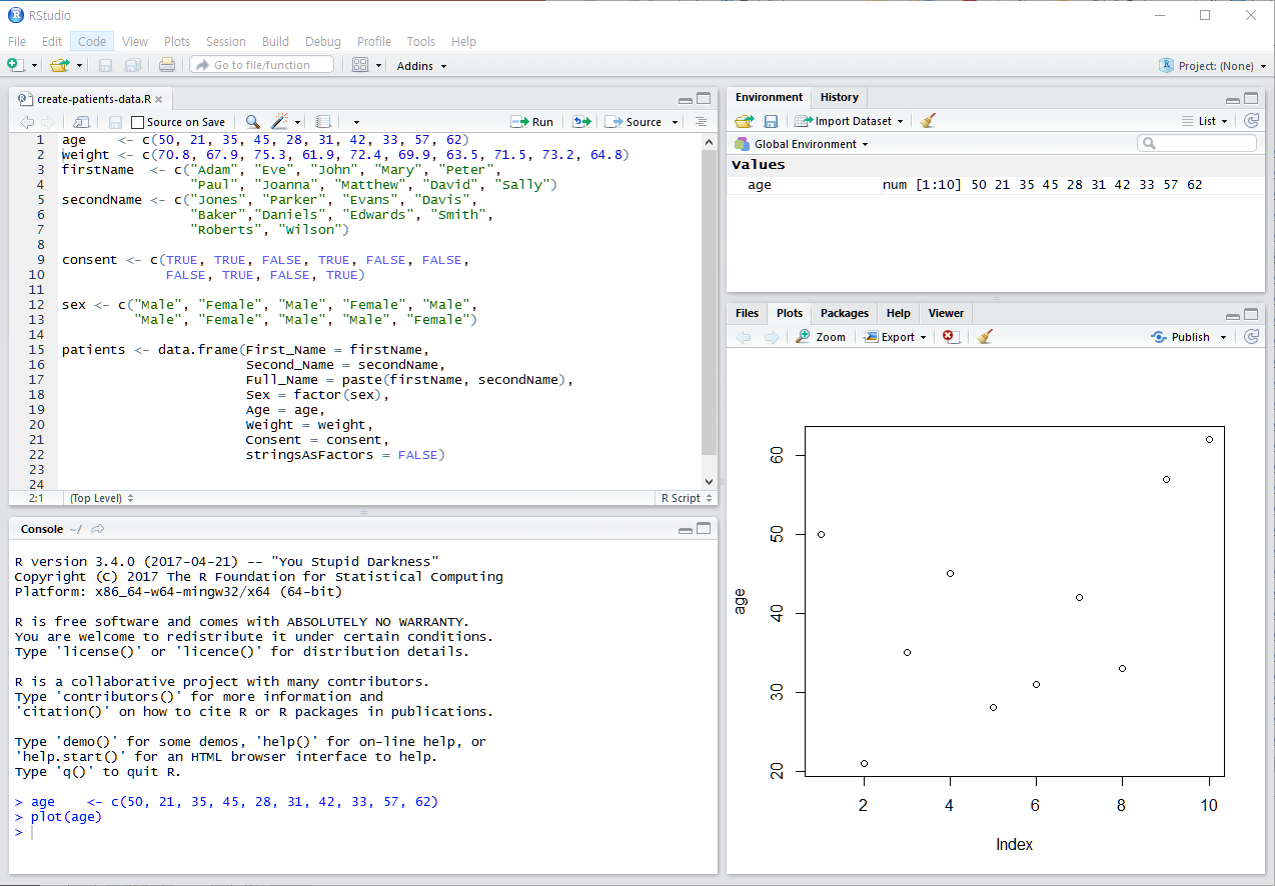
\includegraphics[width=5.20833in,height=\textheight]{images/01/01-11.PNG}

\begin{itemize}
\tightlist
\item
  기본 화면에서 좌측 상단의 공간은 코드편집창, 좌측 하단은 콘솔창
\item
  각 위치를 기호에 따라서 바꿀 수 있음 (View --\textgreater{} Pane)
\end{itemize}

\hypertarget{keyboard-shortcuts}{%
\subsection{Keyboard shortcuts}\label{keyboard-shortcuts}}

\begin{itemize}
\tightlist
\item
  참고사이트

  \begin{itemize}
  \tightlist
  \item
    \url{https://support.rstudio.com/hc/en-us/articles/200711853-Keyboard-Shortcuts}
  \item
    Tools --\textgreater{} Keyboard shortcut Quick Reference (\texttt{Alt\ +\ Shift\ +\ K})
  \end{itemize}
\item
  코드편집창 이동 (\texttt{Ctrl\ +\ 1}) 콘솔창 이동(\texttt{Ctrl\ +\ 2})
\item
  한 줄 실행 (\texttt{Ctrl\ +\ Enter})
\item
  저장 (\texttt{Ctrl\ +\ S})
\item
  주석처리 (\texttt{Ctrl\ +\ Shift\ +\ C})

  \begin{itemize}
  \tightlist
  \item
    또는 \texttt{\#}으로 시작하는 라인
  \end{itemize}
\item
  텝 이동 (\texttt{Ctrl\ +\ F11}, \texttt{Ctrl\ +\ F12})
\item
  코드편집창 확대 (\texttt{Shift\ +\ Ctrl\ +\ 1}) 콘솔창 확대 (\texttt{Shift\ +\ Ctrl\ +\ 2})
\item
  컬럼 편집 (\texttt{Alt\ +\ 마우스\ 드레그})
\item
  자동 완성 기능 (Tab completion) in RStudio
\end{itemize}

\textbf{Exercises}

\begin{enumerate}
\def\labelenumi{\arabic{enumi}.}
\tightlist
\item
  코드편집창에서 다음을 입력/실행하고 단축키를 사용하여 주석을 넣으시오
\end{enumerate}

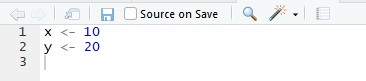
\includegraphics{images/01/01-14.PNG}

\begin{itemize}
\tightlist
\item
  단축키 \texttt{Ctrl\ +\ enter}로 코드 실행
\item
  단축키 \texttt{Ctrl\ +\ 2}로 커서 콘솔창으로 이동
\item
  \texttt{x}값 \texttt{x+y}값 확인
\item
  단축키 \texttt{Ctrl\ +\ 1}로 코드편집창 이동
\item
  단축키 \texttt{Ctrl\ +\ Shift\ +\ C} 사용
\end{itemize}

\begin{Shaded}
\begin{Highlighting}[]
\CommentTok{\# x \textless{}{-} 10}
\CommentTok{\# y \textless{}{-} 20}
\end{Highlighting}
\end{Shaded}

\hypertarget{environment-and-files}{%
\subsection{Environment and Files}\label{environment-and-files}}

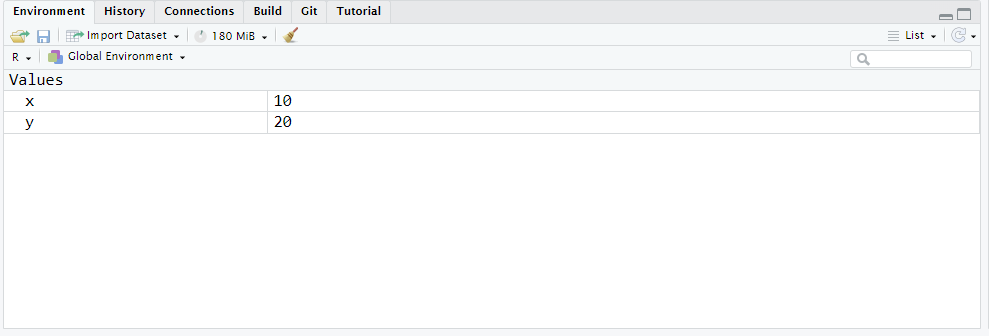
\includegraphics[width=4.16667in,height=\textheight]{images/01/envandhist.png}

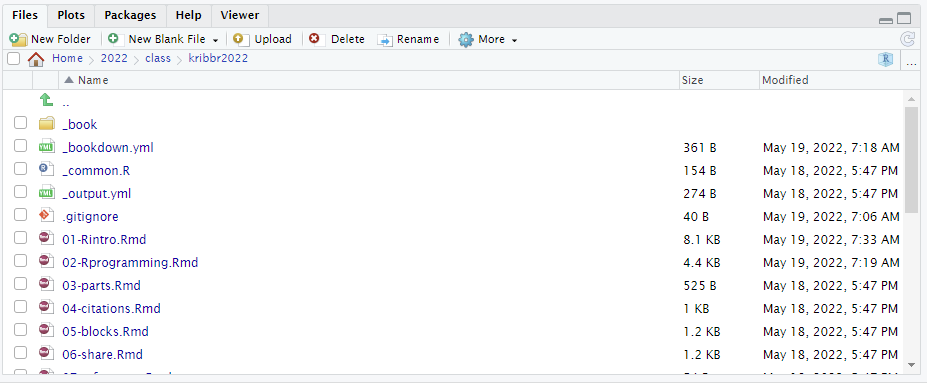
\includegraphics[width=4.16667in,height=\textheight]{images/01/fileandpackages.png}

\hypertarget{start-a-project}{%
\section{Start a project}\label{start-a-project}}

프로젝트를 만들어서 사용할 경우 파일이나 디렉토리, 내용 등을 쉽게 구분하여 사용 가능합니다. 아래와 같이 임의의 디렉토리에 \texttt{kribbR} 이라는 디렉토리를 생성하고 \texttt{lecture1} 프로젝트를 만듭니다.

\begin{quote}
File \textgreater{} New Project \textgreater{} New Directory \textgreater{} New Project \textgreater{} ``kribbR'' \textgreater{} Create Project
\end{quote}

시작할 때는 해당 디렉토리의 \texttt{xxx.Rproj} 파일을 클릭합니다. Rstudio 오른쪽 상단 프로젝트 선택을 통해서 빠르게 다른 프로젝트의 작업공간으로 이동할 수 있습니다.

\hypertarget{hello-world}{%
\subsection{Hello world}\label{hello-world}}

\begin{quote}
File \textgreater{} New File \textgreater{} R markdown \textgreater{} OK
\end{quote}

\begin{Shaded}
\begin{Highlighting}[]
\NormalTok{mystring }\OtherTok{\textless{}{-}} \StringTok{"Hello }\SpecialCharTok{\textbackslash{}n}\StringTok{ world!"}
\FunctionTok{cat}\NormalTok{(mystring)}
\FunctionTok{print}\NormalTok{(mystring)}
\end{Highlighting}
\end{Shaded}

\hypertarget{getting-help}{%
\section{Getting help}\label{getting-help}}

R은 방대한 양의 도움말 데이터를 제공하며 다음과 같은 명령어로 특정 함수의 도움말과 예제를 찾아볼 수 있습니다. \texttt{?} 명령을 사용하면 되며 구글이나 웹에서도 도움을 얻을 수 있습니다.

\begin{Shaded}
\begin{Highlighting}[]
\FunctionTok{help}\NormalTok{(}\StringTok{"mean"}\NormalTok{)}
\NormalTok{?mean}
\FunctionTok{example}\NormalTok{(}\StringTok{"mean"}\NormalTok{)}
\FunctionTok{help.search}\NormalTok{(}\StringTok{"mean"}\NormalTok{)}
\NormalTok{??mean}
\FunctionTok{help}\NormalTok{(}\AttributeTok{package=}\StringTok{"MASS"}\NormalTok{)}
\end{Highlighting}
\end{Shaded}

또한 \url{https://www.rstudio.com/resources/cheatsheets/} 에서는 다양한 R언어의 기능을 한 눈에 알아볼 수 있게 만든 cheatsheet 형태의 문서를 참고할 수 있습니다.

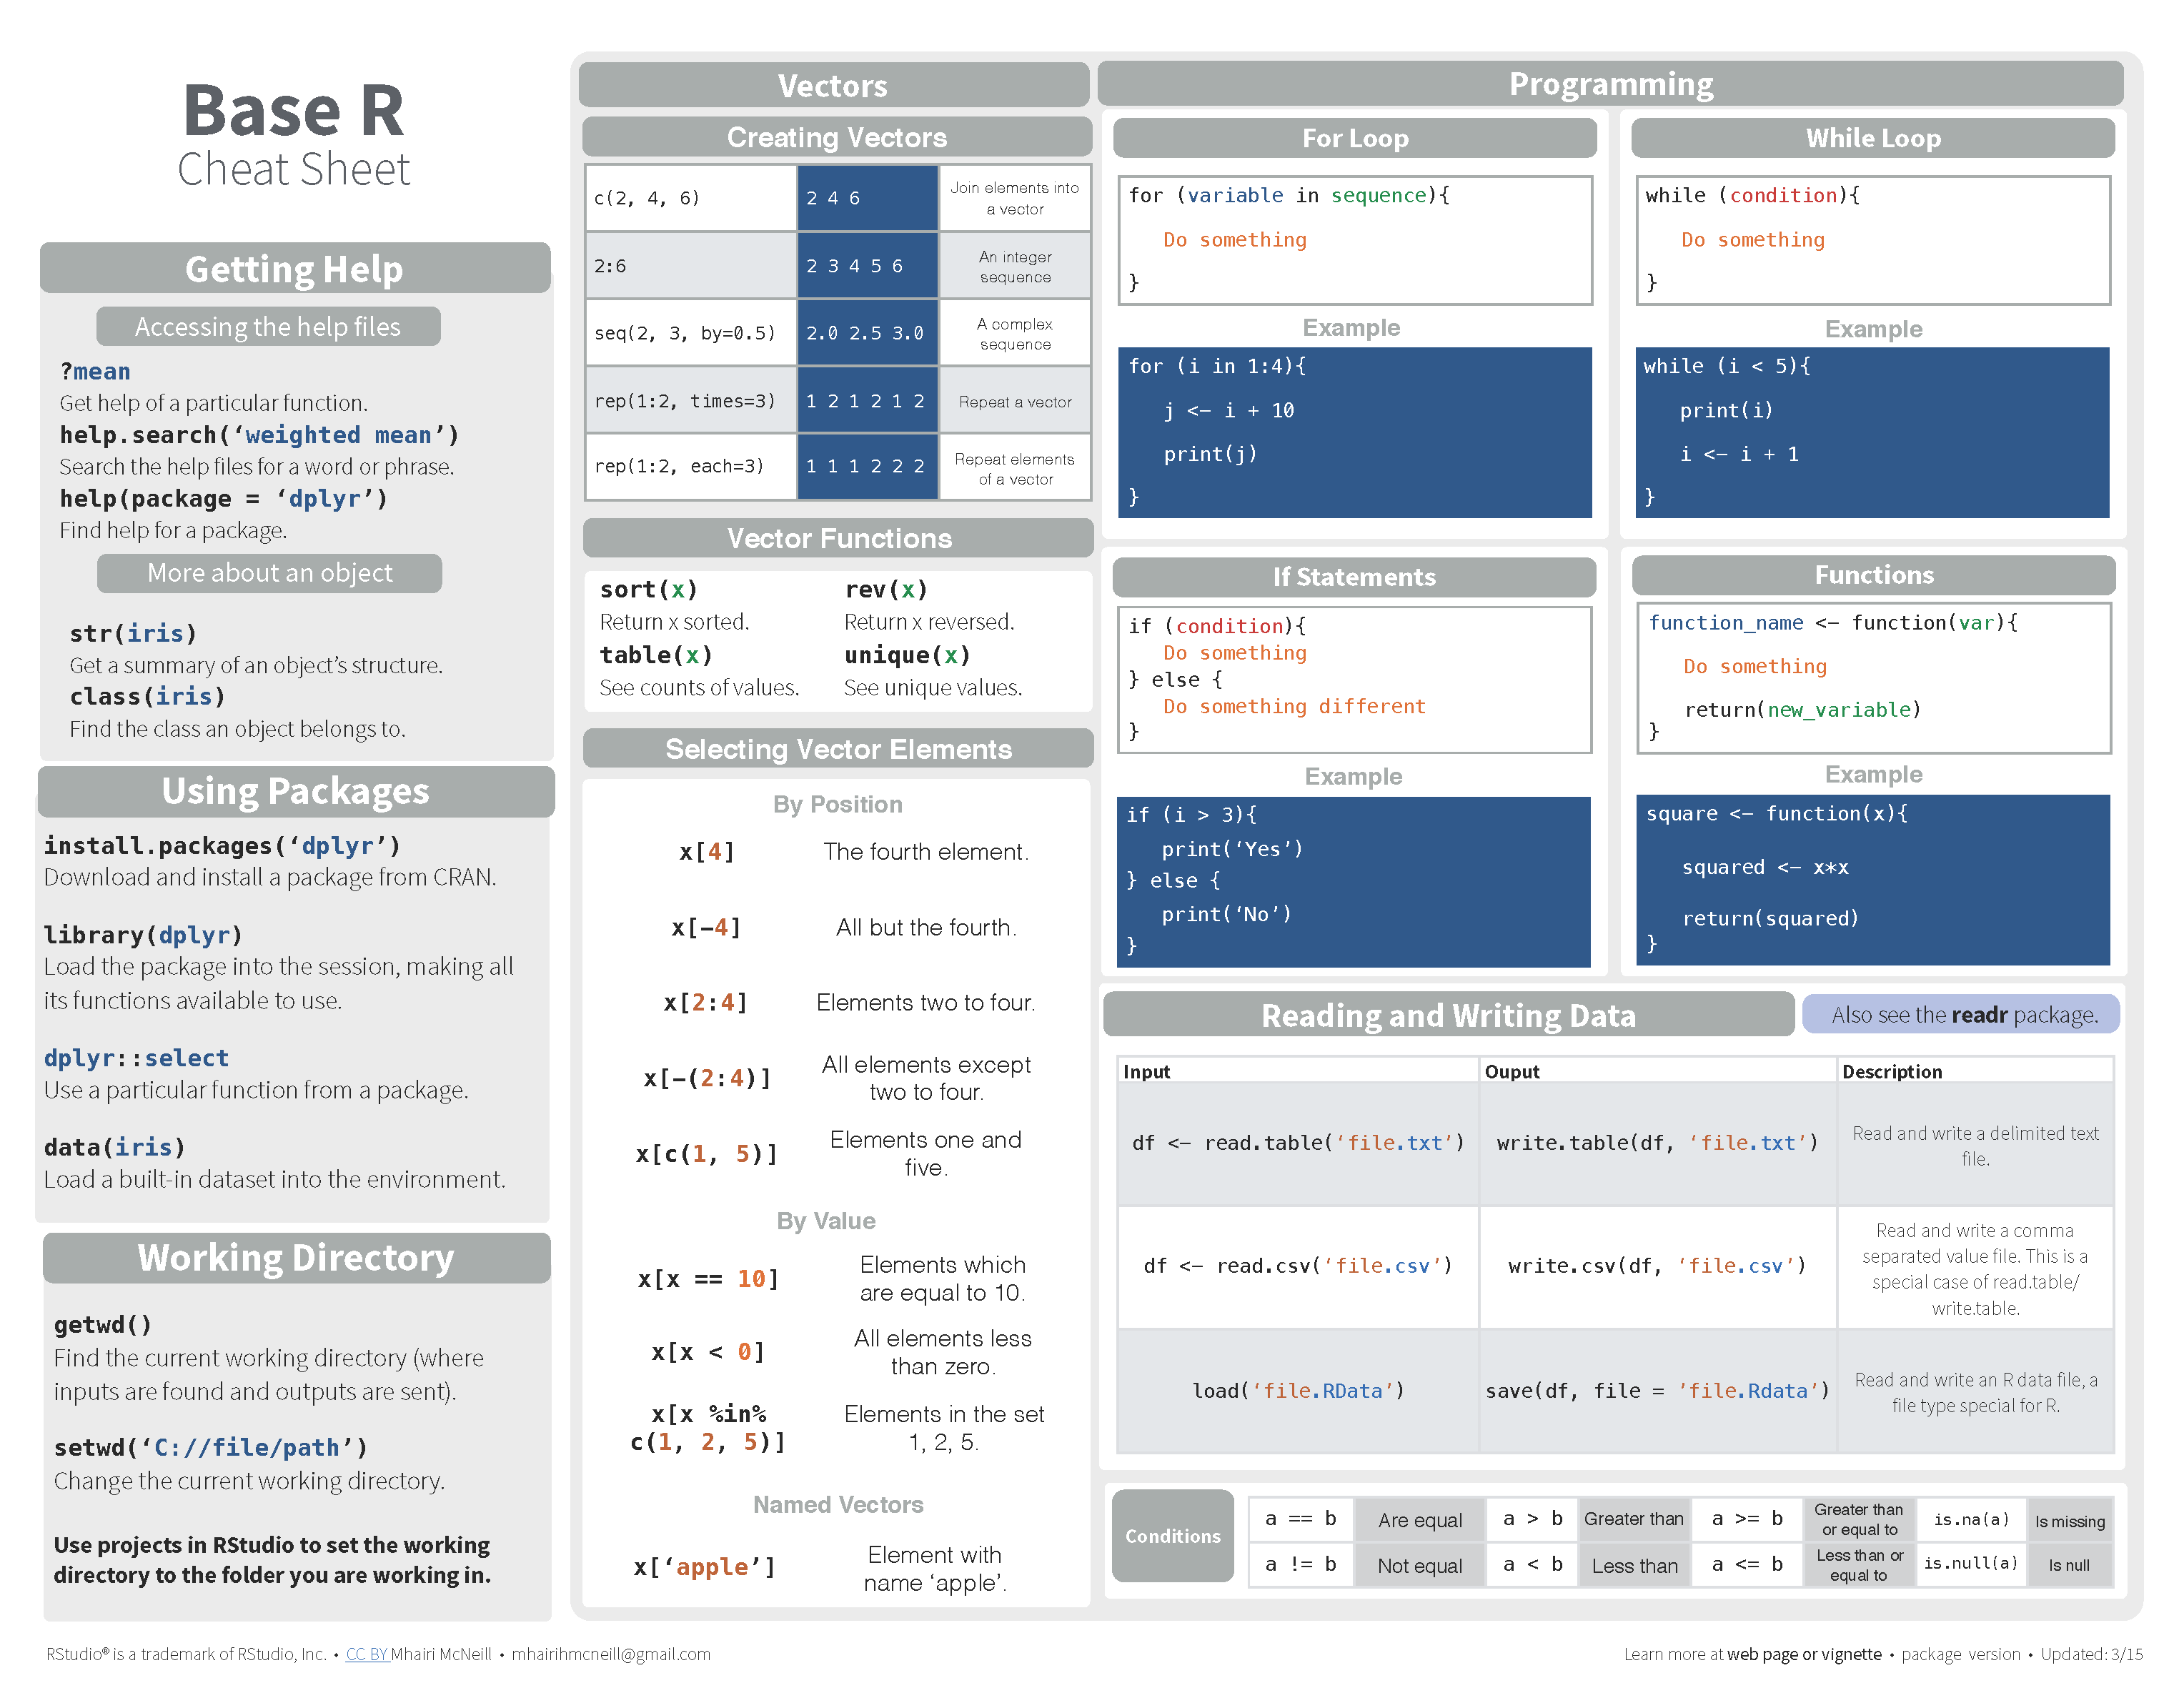
\includegraphics[width=5.72917in,height=\textheight]{images/01/base-r_1.png}
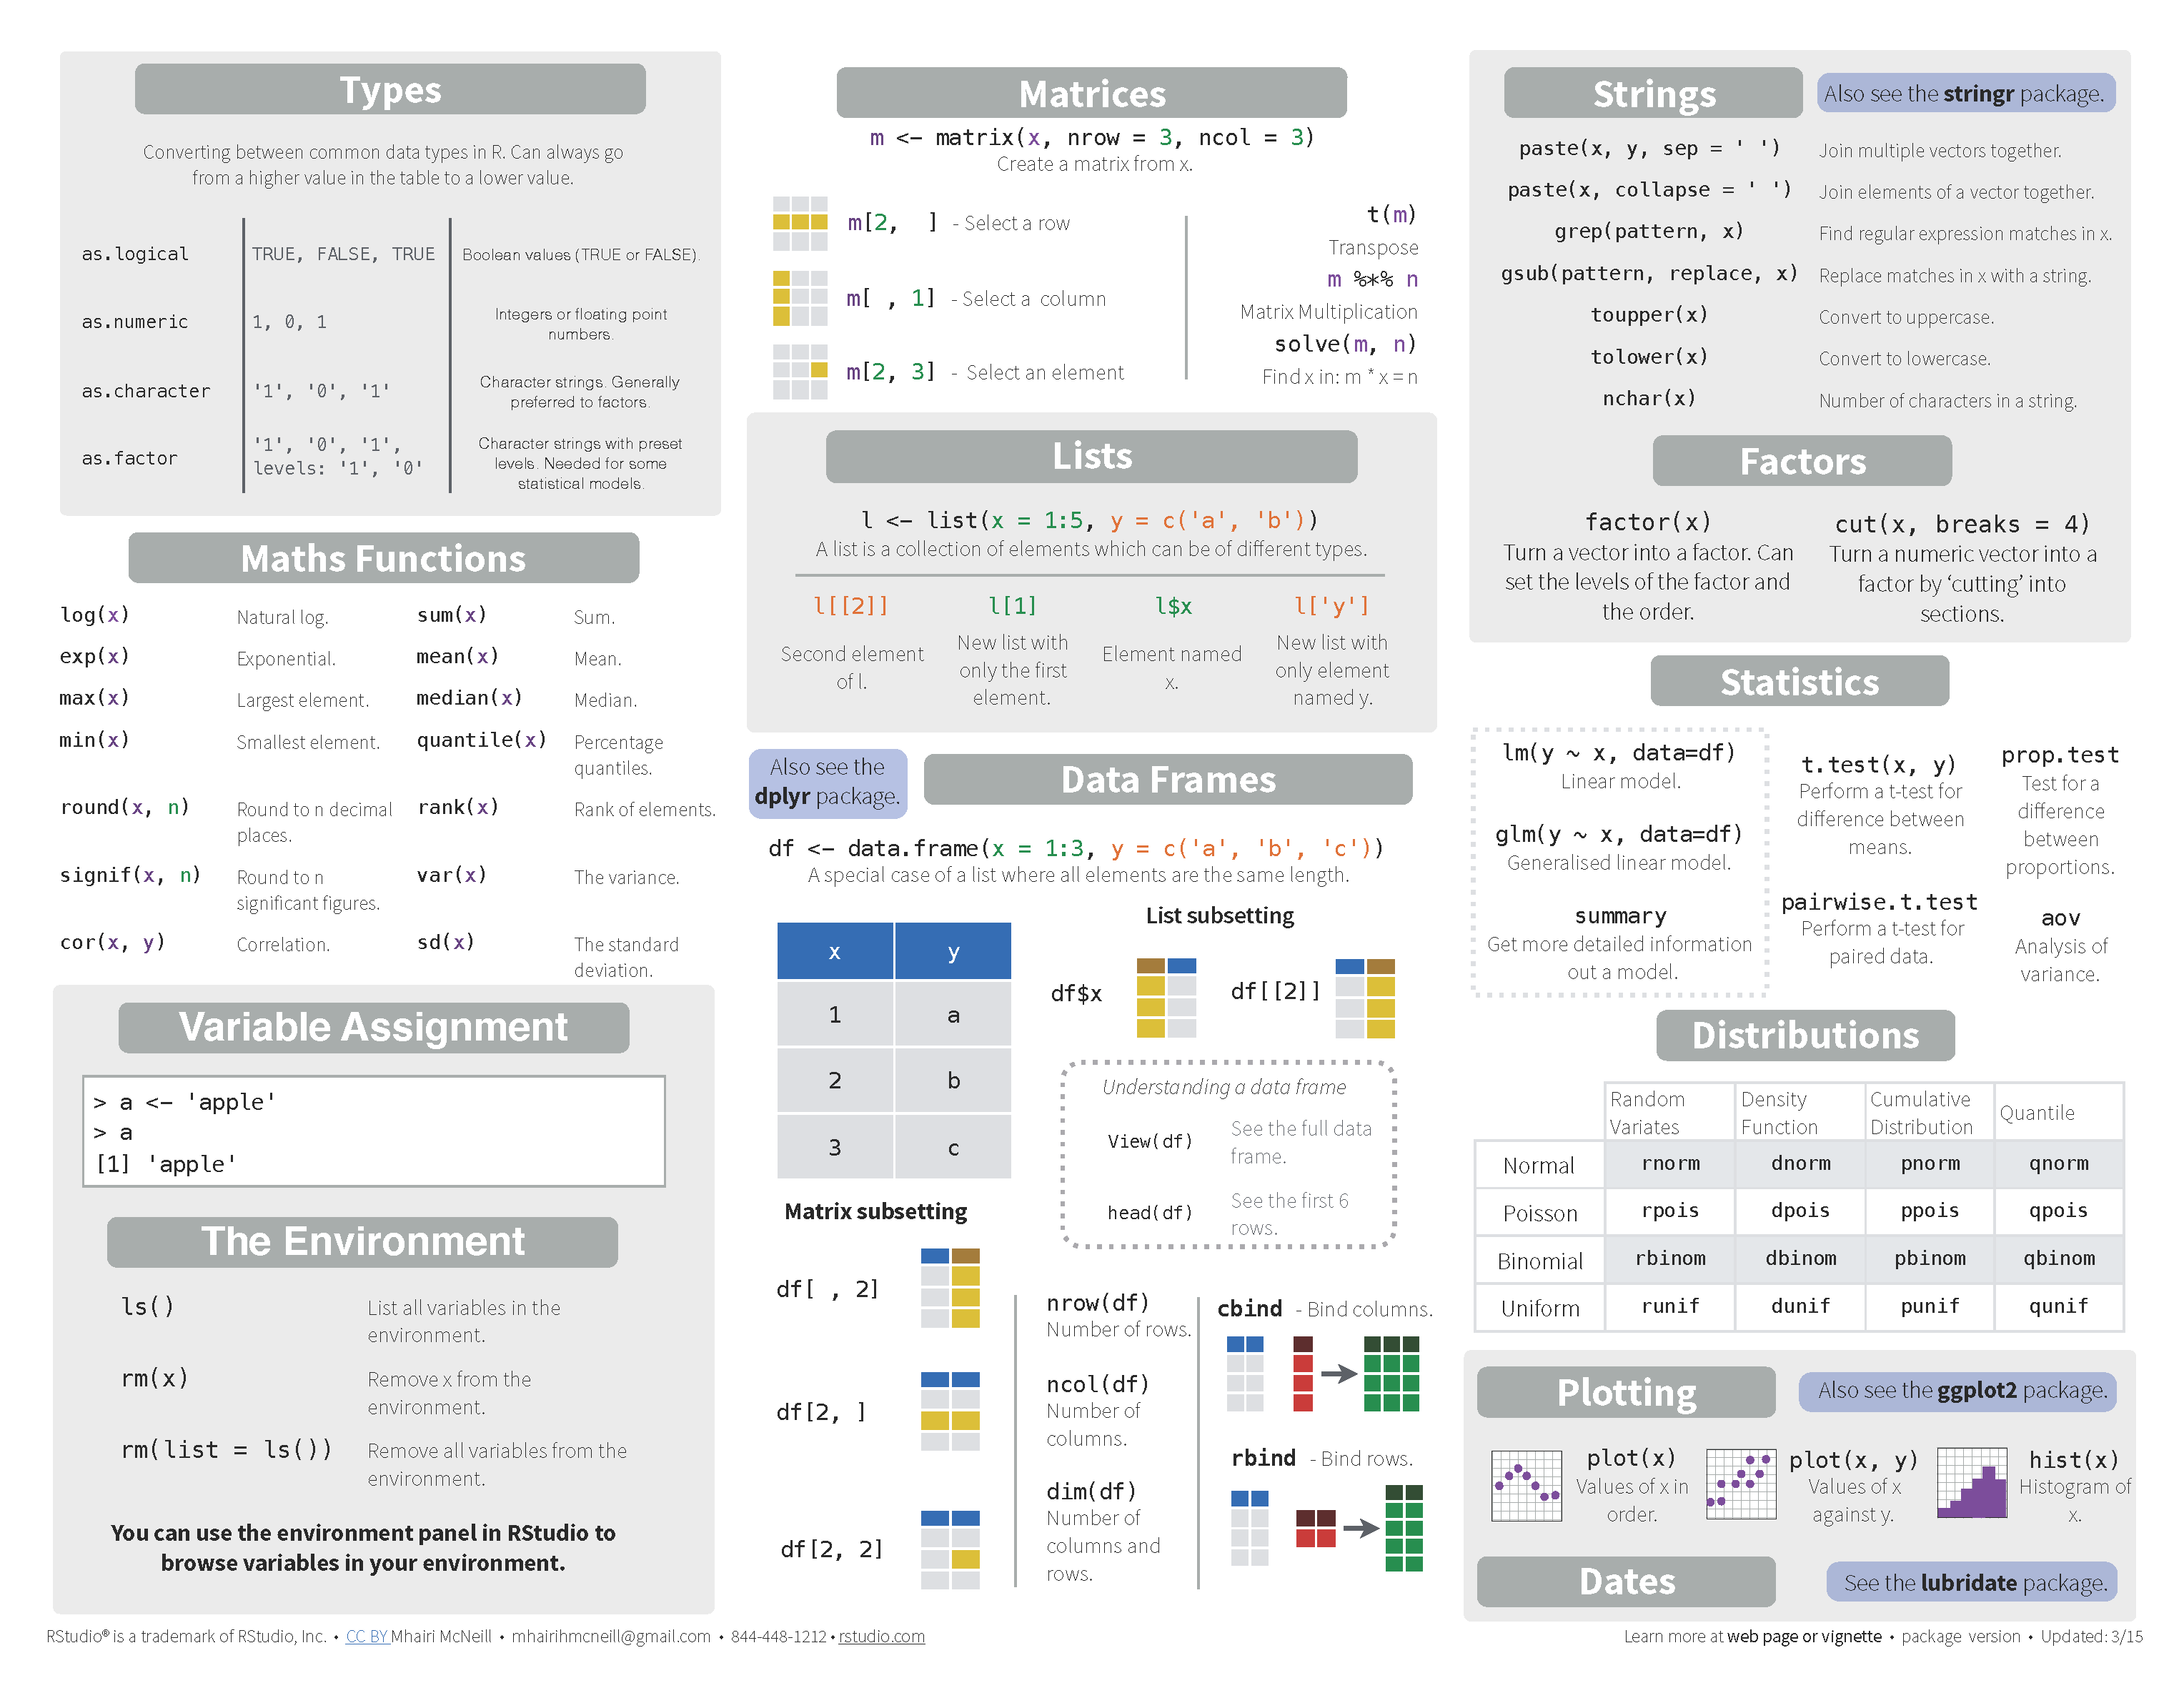
\includegraphics[width=5.72917in,height=\textheight]{images/01/base-r_2.png}

\hypertarget{r-packages-and-dataset}{%
\section{R packages and Dataset}\label{r-packages-and-dataset}}

R 패키지는 함수와 데이터셋의 묶음으로 다른 사람들이 만들어 놓은 코드나 기능을 가져와서 사용하므로써 코드 작성의 수고로움을 줄이고 편리하고 검증된 함수(기능)를 빠르게 도입하여 사용할 수 있다는 장점이 있습니다. 예를 들어 \texttt{sd()} 함수는 \texttt{stats} package에서 제공하는 함수로써 표준편차 계산을 위한 별도의 함수를 만들어서 사용할 필요가 없이 바로 (stats 패키지는 R 기본 패키지로) 별도 설치 없이 바로 사용 가능합니다.

이러한 패키지는 인터넷의 \texttt{repository}에서 구할 수 있으며 대표적인 \texttt{repository}는 The Comprehensive R Archive Network (CRAN) (\url{http://cran.r-project.org/web/views/}) 와 생물학자를 위한 Bioconductor (\url{http://www.bioconductor.org/}) 가 있습니다. 이러한 패키지의 설치는 아래와 같이 RStudio를 이용하거나 콘솔창에서 \texttt{install.packages()} 함수를 이용할 수 있습니다.

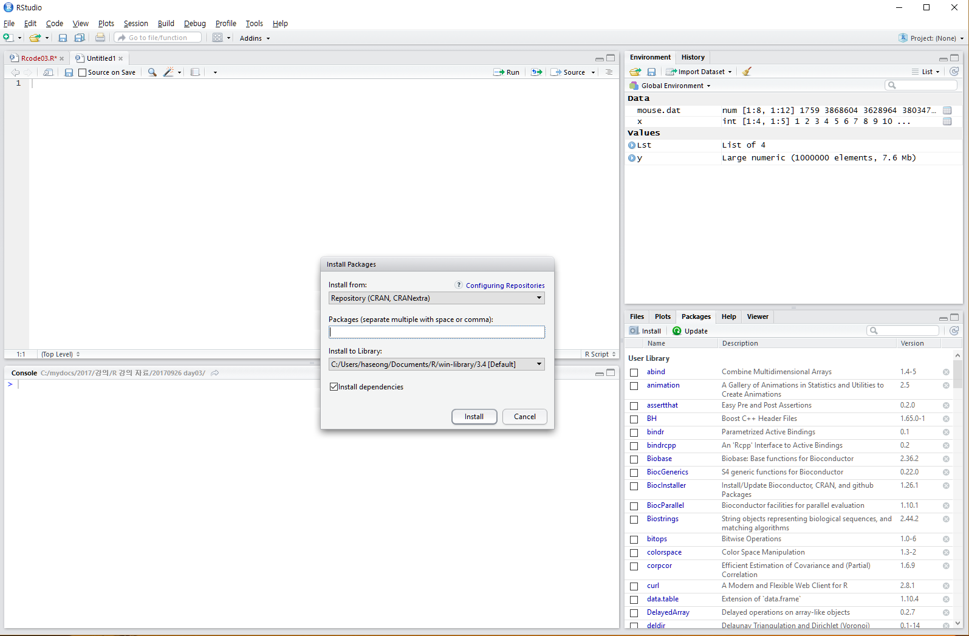
\includegraphics[width=4.6875in,height=\textheight]{images/01/01-18.PNG}

패키지를 설치하고 사용하기 위해서는 \texttt{library()} 함수를 사용해서 관련 명령어를 사용하기 전에 미리 loading 해 두어야 합니다. 한 번 로딩으로 작업 세션이 끝날때까지 관련된 함수를 사용할 수 있으나 R 세션이나 RStudio를 재시작 할 경우 다시 로딩해야 사용할 수 있습니다.

\begin{Shaded}
\begin{Highlighting}[]
\FunctionTok{library}\NormalTok{(UsingR)}
\end{Highlighting}
\end{Shaded}

\begin{itemize}
\tightlist
\item
  R 설치 디렉토리
\item
  R 패키지 설치 디렉토리
\end{itemize}

\begin{Shaded}
\begin{Highlighting}[]
\FunctionTok{.libPaths}\NormalTok{()}
\FunctionTok{path.package}\NormalTok{()}
\end{Highlighting}
\end{Shaded}

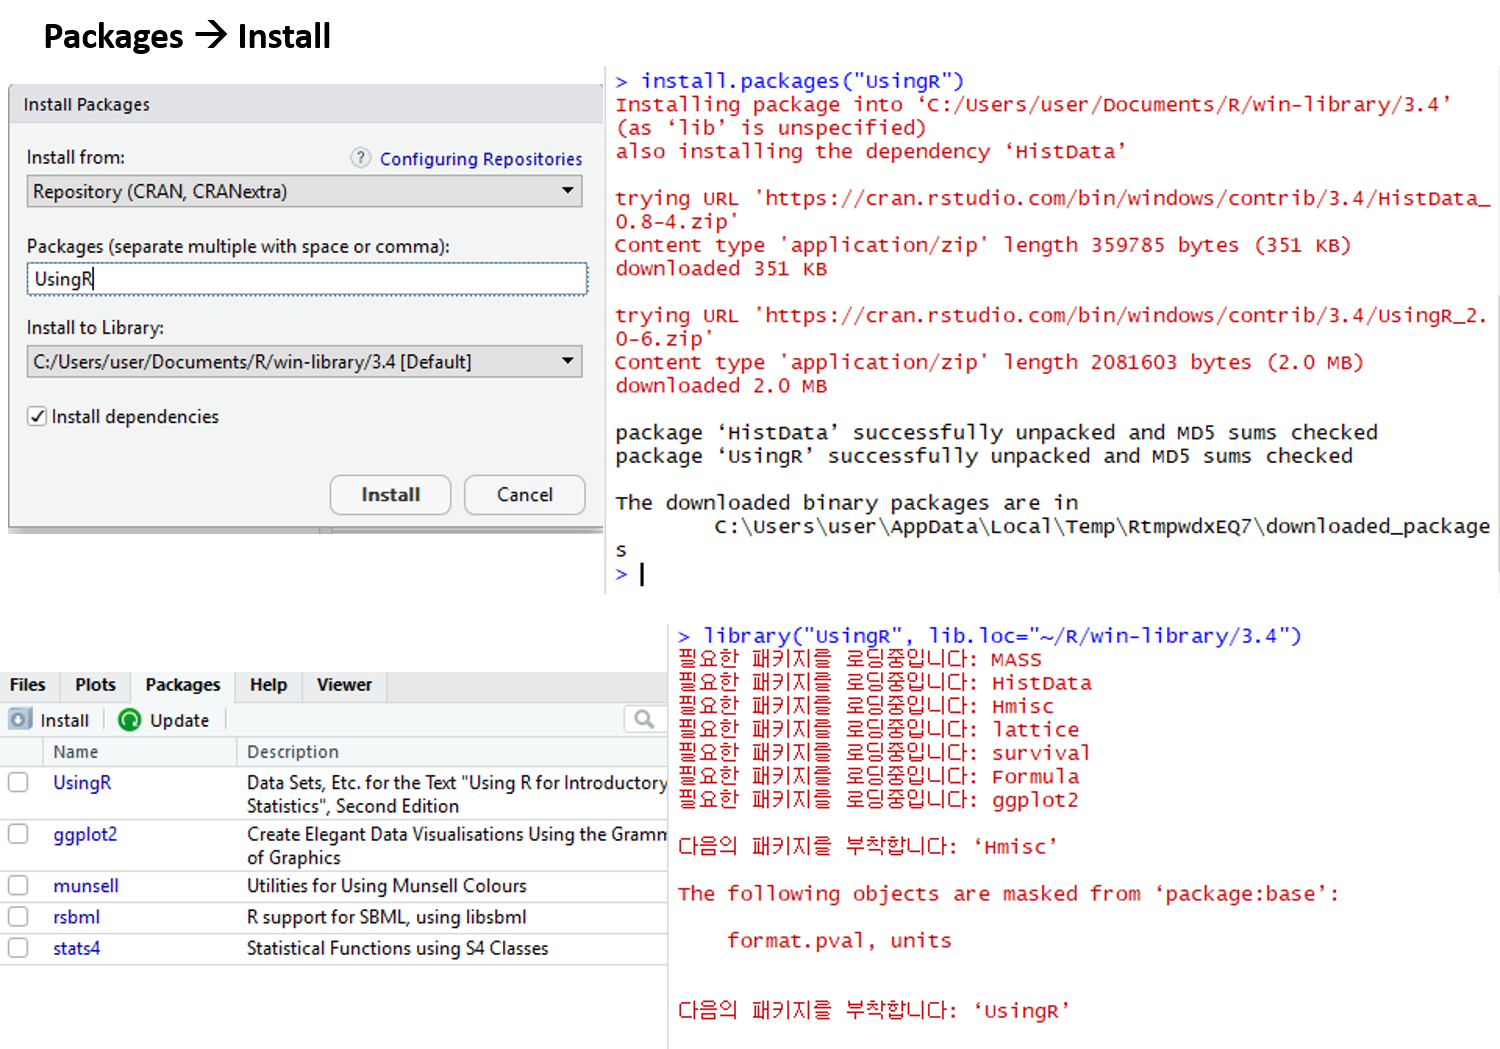
\includegraphics[width=4.6875in,height=\textheight]{images/01/01-19.PNG}

일반적으로 패키지 안에 관련된 데이터도 같이 저장되어 있으며 \texttt{data()} 함수를 이용해서 패키지 데이터를 사용자 작업공간에 복사해서 사용 가능합니다.

\begin{Shaded}
\begin{Highlighting}[]
\FunctionTok{head}\NormalTok{(rivers)}
\FunctionTok{length}\NormalTok{(rivers)}
\FunctionTok{class}\NormalTok{(rivers)}
\FunctionTok{data}\NormalTok{(rivers)}
\FunctionTok{data}\NormalTok{(}\AttributeTok{package=}\StringTok{"UsingR"}\NormalTok{)}
\FunctionTok{library}\NormalTok{(HistData)}
\FunctionTok{head}\NormalTok{(Cavendish)}
\FunctionTok{str}\NormalTok{(Cavendish)}
\FunctionTok{head}\NormalTok{(Cavendish}\SpecialCharTok{$}\NormalTok{density2)}
\end{Highlighting}
\end{Shaded}

\begin{center}\rule{0.5\linewidth}{0.5pt}\end{center}

이 저작물은 크리에이티브 커먼즈 저작자표시-비영리-변경금지 4.0 국제 라이선스에 따라 이용할 수 있습니다.

\hypertarget{rmarkdown}{%
\chapter{Rmarkdown}\label{rmarkdown}}

Rmarkdown은 데이터를 분석하는 코드와 리포트를 동시에 수행할 수 있는 일종의 통합 문서입니다. 워드나 아래한글에서 프로그래밍과 데이터분석을 위한 코드를 작성할 수 있는 경우라고 생각해도 됩니다. Plain-text 기반의 markdown 문법을 사용하며 Rmarkdown으로 작성된 문서는 HTML, PDF, MS word, Beamer, HTML5 slides, books, website 등 다양한 포멧의 출력물로 변환할 수 있습니다.

\begin{figure}
\centering
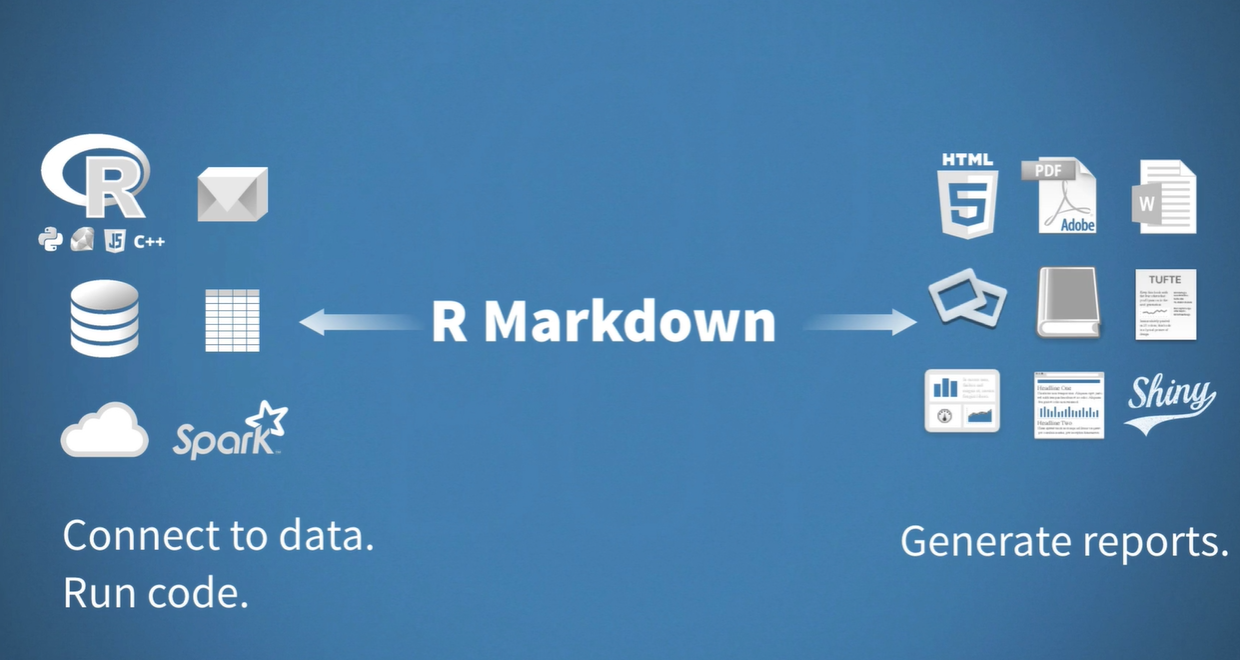
\includegraphics[width=5.20833in,height=\textheight]{images/rmarkdown/rmarkdown-01.PNG}
\caption{Image from rmarkdown.rstudio.com}
\end{figure}

Rmarkdown 웹사이트에 Rmarkdown 소개 동영상과 \href{https://rmarkdown.rstudio.com/lesson-1.html}{Rmarkdown 공식 사이트 메뉴얼} 관련 서적 \href{https://bookdown.org/yihui/rmarkdown/}{Rmarkdown: The Definitive Guide}를 참고하세요. 또한 Rmarkdown을 사용할 때 \href{https://github.com/rstudio/cheatsheets/raw/master/rmarkdown-2.0.pdf}{cheatsheet}를 옆에 두고 수시로 보면서 사용하시면 많은 도움이 될 수 있습니다.

\hypertarget{rmarkdownuxc758-uxae30uxbcf8-uxc791uxb3d9-uxc6d0uxb9ac}{%
\section{Rmarkdown의 기본 작동 원리}\label{rmarkdownuxc758-uxae30uxbcf8-uxc791uxb3d9-uxc6d0uxb9ac}}

Rmarkdown은 plain text 기반으로 작성되며 Rmd 라는 확장자를 갖는 파일로 저장됩니다. 다음과 같은 텍스트 파일이 Rmd 파일의 전형적인 예 입니다.

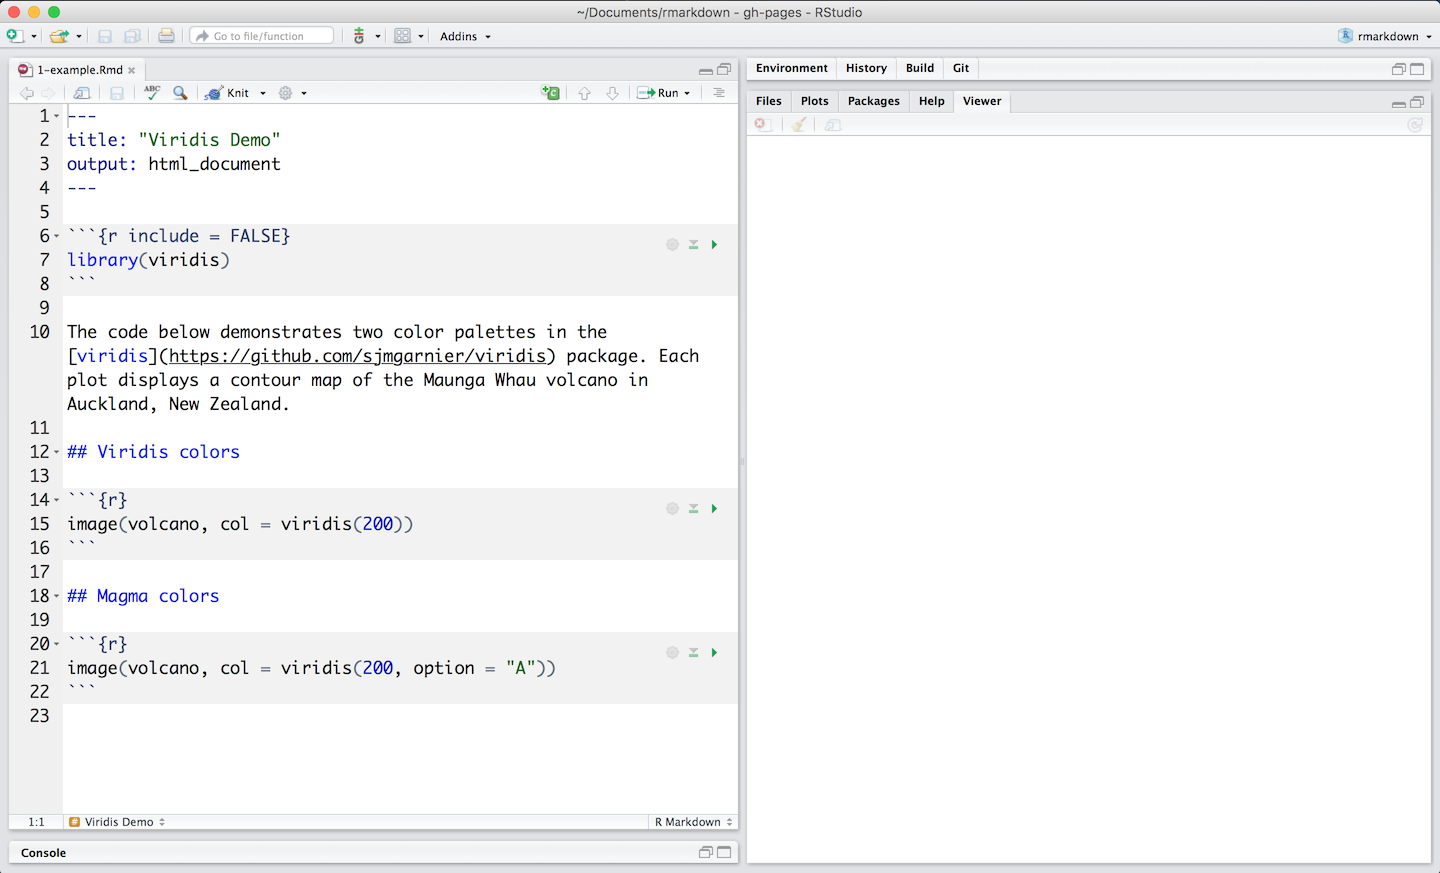
\includegraphics[width=5.20833in,height=\textheight]{images/rmarkdown/how-1-file.png}

위 예제에서 네 가지 다른 종류의 컨텐츠를 볼 수 있습니다. 하나는 - - - 으로 둘러쌓인 내용으로 YAML 이라고 하며 JSON과 같은 데이터 직렬화를 수행하는 하나의 데이터 저장 포멧입니다. 백틱(`) 으로 둘러쌓인 코드청그(Code Chunks)라고 하는 부분에는 R이나 python 등의 다양한 코드(실재 작동하는)를 넣어서 사용합니다. 그리고 \#\#\# 으로 표시된 글은 제목 글을 나타내며 나머지는 일반적인 텍스트를 나타냅니다.

이러한 Rmarkdown 파일은 \texttt{render}라는 명령어로 원하는 포맷의 문서로 변환할 수 있습니다. 다음 예의 파일을 pdf 형식으로 rendering 하기 위해서는 YAML에 pdf 임을 명시하고 아래와 같이 \texttt{render}함수를 사용하면 됩니다. 또는 Rstudio 코드 입력창 상단의 Knit 버튼으로 pdf나 html 문서를 생성할 수 있습니다.

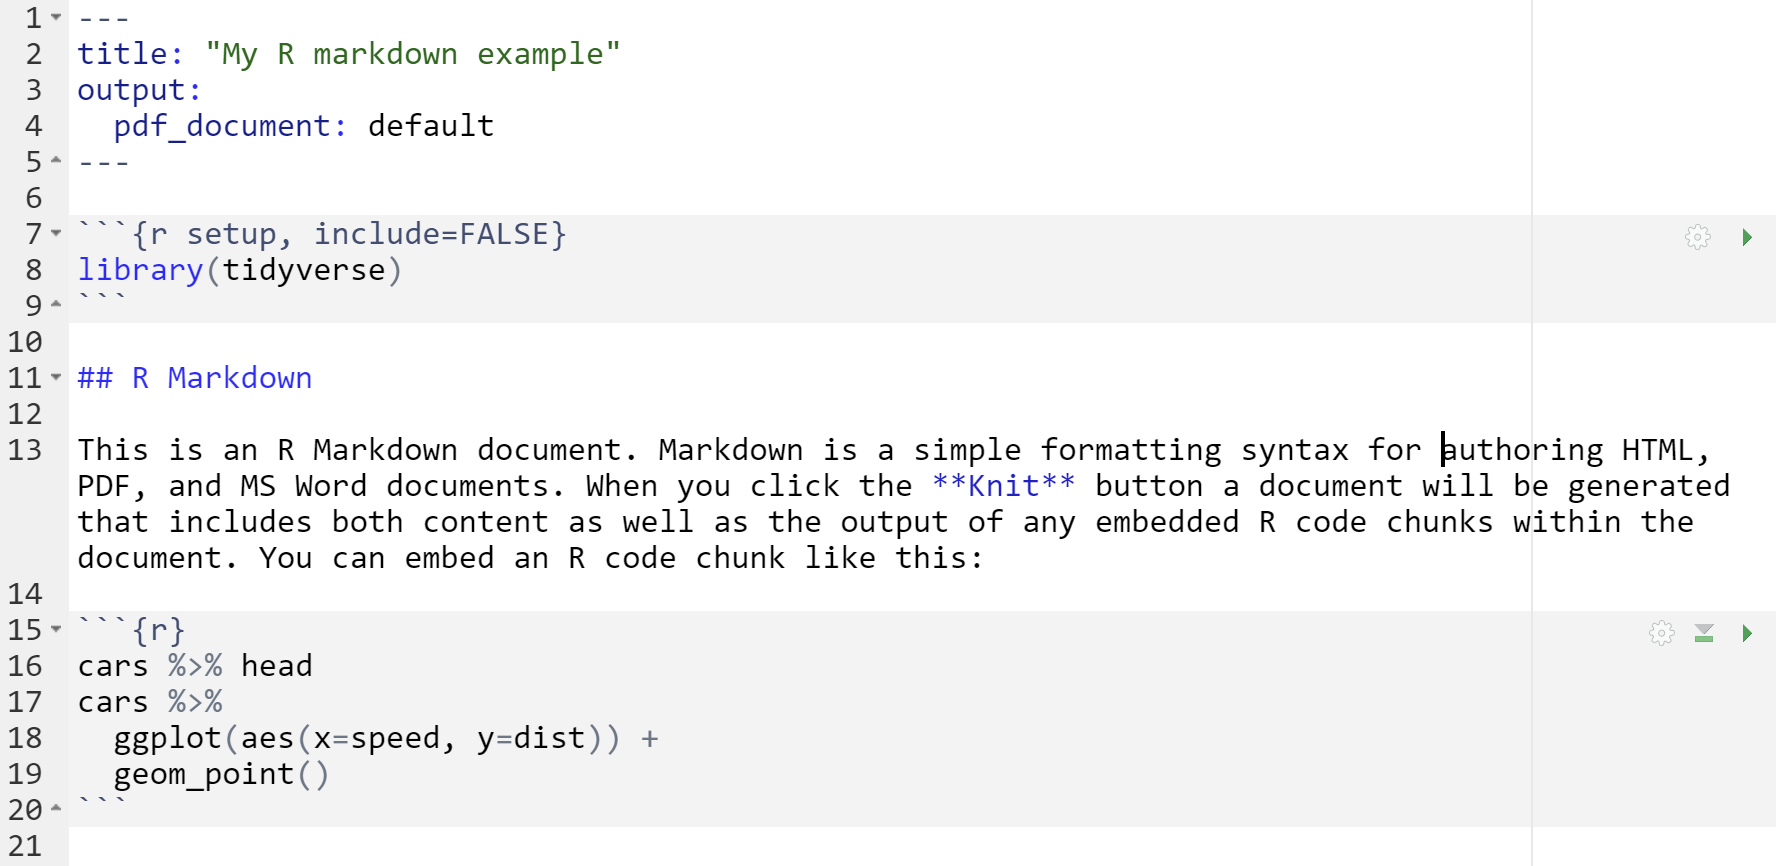
\includegraphics[width=5.20833in,height=\textheight]{images/rmarkdown/example2.PNG}

\begin{Shaded}
\begin{Highlighting}[]
\FunctionTok{render}\NormalTok{(}\StringTok{"examples/test.Rmd"}\NormalTok{, }\AttributeTok{output\_format =} \StringTok{"pdf\_document"}\NormalTok{)}
\end{Highlighting}
\end{Shaded}

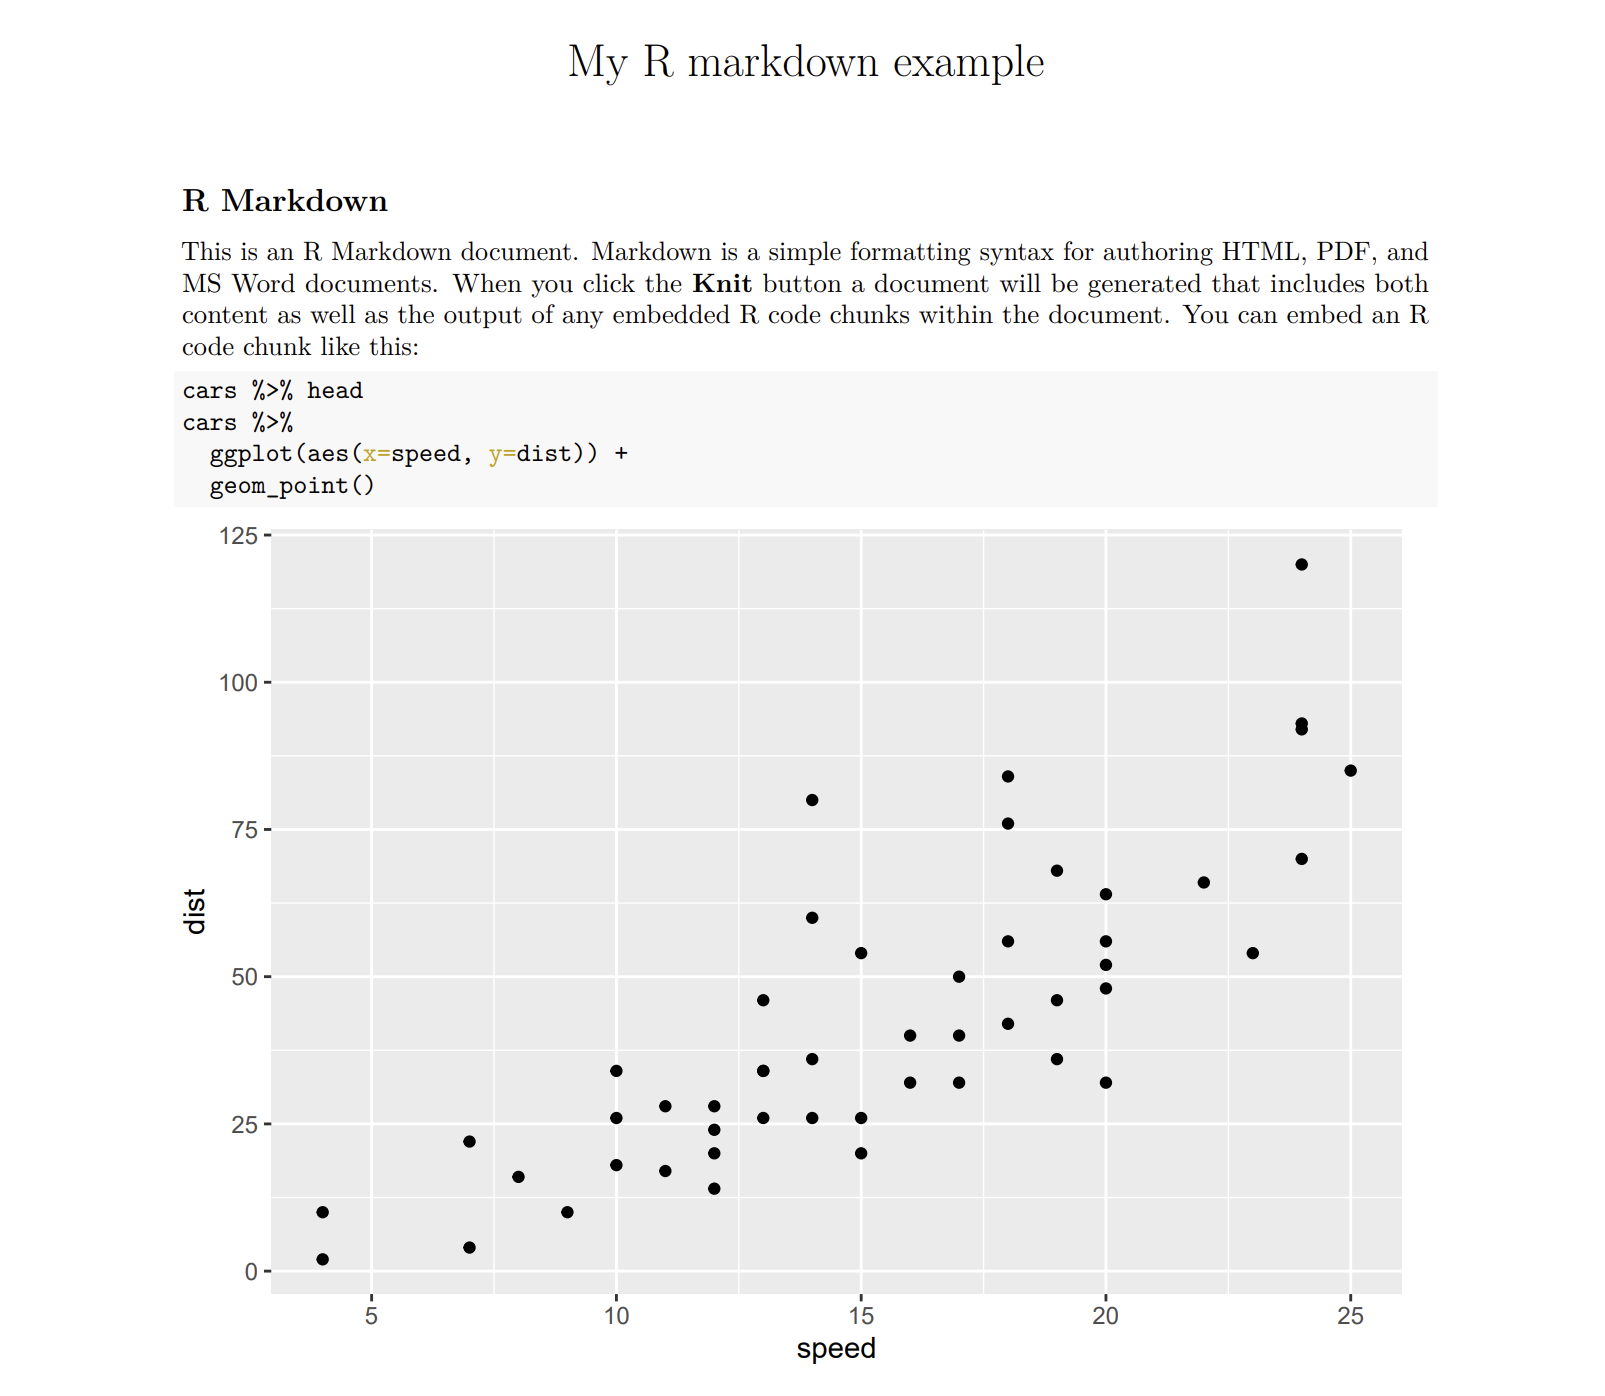
\includegraphics[width=4.6875in,height=\textheight]{images/rmarkdown/ex_pdf.PNG}

Rmarkdown의 작동 원리는 Rmd 파일을 만든 후 \texttt{render} 함수를 부르면 \href{https://yihui.org/knitr/}{knitr} 소프트웨어가 R 코드를 실행시킨 후 markdown (.md) 파일을 생성합니다. 이 후 .md 파일을 \href{https://pandoc.org/}{pandoc} 이라는 문서변환기가 원하는 문서 형태로 전환해 줍니다.

\hypertarget{uxcf54uxb4dc-uxc785uxb825}{%
\section{코드 입력}\label{uxcf54uxb4dc-uxc785uxb825}}

Rmarkdown에서 사용하는 코드청크는 \texttt{CTRL+ALT+i} 단축키를 사용해서 넣을 수 있으며 다음과 같은 몇 가지 옵션으로 코드 스니펫들의 실행/숨김 여부를 결정할 수 있습니다.

\begin{itemize}
\tightlist
\item
  \texttt{include\ =\ FALSE} : 코드는 실행되지만 보고서에 결과와 코드가 보여지지 않음
\item
  \texttt{echo\ =\ FALSE} : 코드는 실행되고 보고서에 결과가 포함되지만 코드는 보여지지 않음
\item
  \texttt{eval\ =\ FALSE} : 코드가 실행되지 않지만 보고서에 코드는 보여짐
\item
  \texttt{message\ =\ FALSE}, \texttt{warning=FALSE}, \texttt{error=FALSE} : 코드에 의해서 발생되는 메세지/경고/에러가 보고서에 보여지지 않음
\item
  \texttt{fig.cap\ =\ "..."} : 코드로 그려지는 그래프에 캡션을 붙일 수 있음
\end{itemize}

\begin{figure}
\centering
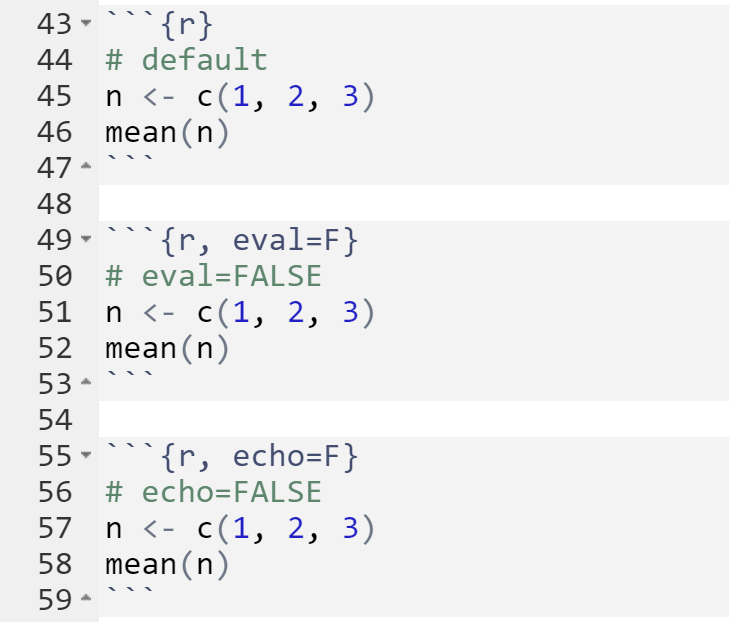
\includegraphics[width=2.60417in,height=\textheight]{images/rmarkdown/codechunk1.PNG}
\caption{코드청크 옵션 예시}
\end{figure}

실행 결과는 아래와 같습니다.

\begin{Shaded}
\begin{Highlighting}[]
\CommentTok{\# default}
\NormalTok{n }\OtherTok{\textless{}{-}} \FunctionTok{c}\NormalTok{(}\DecValTok{1}\NormalTok{, }\DecValTok{2}\NormalTok{, }\DecValTok{3}\NormalTok{)}
\FunctionTok{mean}\NormalTok{(n)}
\CommentTok{\#\textgreater{} [1] 2}
\end{Highlighting}
\end{Shaded}

\begin{Shaded}
\begin{Highlighting}[]
\CommentTok{\# eval=FALSE}
\NormalTok{n }\OtherTok{\textless{}{-}} \FunctionTok{c}\NormalTok{(}\DecValTok{1}\NormalTok{, }\DecValTok{2}\NormalTok{, }\DecValTok{3}\NormalTok{)}
\FunctionTok{mean}\NormalTok{(n)}
\end{Highlighting}
\end{Shaded}

\begin{verbatim}
#> [1] 2
\end{verbatim}

Rmarkdown에서는 ` r`을 사용해서 코드청크가 아닌 곳에 R 코드를 넣을 수 있습니다. 또한 R 언어 외에도 \texttt{Python}, \texttt{SQL}, \texttt{Bash}, \texttt{Rcpp}, \texttt{Stan}, \texttt{JavaScript}, \texttt{CSS} 등의 다양한 프로그래밍 언어에 대해서도 코드청크 기능을 사용할 수 있습니다. 그런데 이러한 언어들이 사용 가능해지기 위해서는 해당 언어들을 실행해주는 엔진이 있어야 하며 python의 경우 \texttt{reticulate} 라는 패키지가 이러한 기능을 담당합니다. 이 패키지를 설치할 경우 miniconda라는 가상환경 및 데이터 분석을 위한 오픈소스 패키지가 자동으로 설치됩니다.

\begin{Shaded}
\begin{Highlighting}[]
\FunctionTok{library}\NormalTok{(reticulate)}
\end{Highlighting}
\end{Shaded}

\begin{Shaded}
\begin{Highlighting}[]
\NormalTok{x }\OperatorTok{=} \StringTok{"hello, python in R"}
\BuiltInTok{print}\NormalTok{(x.split(}\StringTok{\textquotesingle{} \textquotesingle{}}\NormalTok{))}
\end{Highlighting}
\end{Shaded}

아래는 위에 해당하는 소스코드 입니다.

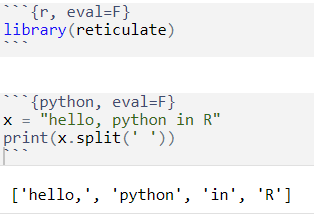
\includegraphics[width=2.60417in,height=\textheight]{images/02/lecticulate.png}

\hypertarget{markdown-uxbb38uxbc95}{%
\section{Markdown 문법}\label{markdown-uxbb38uxbc95}}

마크다운은 plain text 기반의 마크업 언어로서 마크업 언어는 태그 등을 이용해서 문서의 데이터 구조를 명시하는데 이러한 태그를 사용하는 방법 체계를 마크업 언어라고 합니다. 가장 대표적으로 html 이 있습니다.

\begin{verbatim}
    <html>
      <head>
        <title> Hello HTML </title>
      </head>
      <body>
      Hello markup world!
      </body>
    </html>
\end{verbatim}

마크다운도 몇 가지 태그를 이용해서 문서의 구조를 정의하고 있으며 상세한 내용은 \href{https://rmarkdown.rstudio.com/authoring_pandoc_markdown.html}{Pandoc 마크다운 문서}를 참고하시기 바랍니다. 마크다운언어의 철학은 쉽게 읽고 쓸 수 있는 문서입니다. plain text 기반으로 작성되어 쓰기 쉬우며 (아직도 사람들이 메모장 많이 사용하는 이유와 같습니다) 태그가 포함되어 있어도 읽는데 어려움이 없습니다. 위 html 언어와 아래 markdown 파일의 예들을 보시면 그 차이를 어렵지 않게 이해할 수 있습니다.

마크다운에서는 Enter를 한 번 입력해서 줄바꿈이 되지 않습니다. \texttt{\textless{}br\textgreater{}} 또는 문장 마지막에 공백을 두 개 입력하면 되겠습니다.

\begin{verbatim}
이 문장은 줄바꿈이 
되지 않습니다
\end{verbatim}

이 문장은 줄바꿈이
되지 않습니다

\begin{verbatim}
이 분장은 줄바꿈이<br>
됩니다
\end{verbatim}

이 분장은 줄바꿈이
됩니다

마크다운 테그를 몇 가지 살펴보면 먼저 \# 을 붙여서 만드는 header 가 있습니다.

\begin{verbatim}
# A level-one header
## A level-two header
### A level-three header

# A level-one header {#l1-1}
## A level-two header {#l2-1}
### A level-three header {#l3-1}

# A level-one header {#l1-2}
## A level-two header {#l2-2}
### A level-three header {#l3-2}
\end{verbatim}

Block quotations

\begin{quote}
This is block quote. This paragraph has two lines
\end{quote}

\begin{verbatim}
> This is block quote. This paragraph has two lines
\end{verbatim}

\begin{quote}
This is a block quote.

\begin{quote}
A block quote within a block quote.
\end{quote}
\end{quote}

\begin{verbatim}
> This is a block quote.
>
> > A block quote within a block quote.
\end{verbatim}

\emph{Italic}

\begin{verbatim}
*Italic*
\end{verbatim}

\textbf{Bold}

\begin{verbatim}
**Bold**
\end{verbatim}

\href{https://www.naver.com/}{Naver link}

\begin{verbatim}
[Naver link](https://www.naver.com/)
\end{verbatim}

이미지를 직접 삽입하고 가운데 정렬합니다.

\begin{figure}
\centering
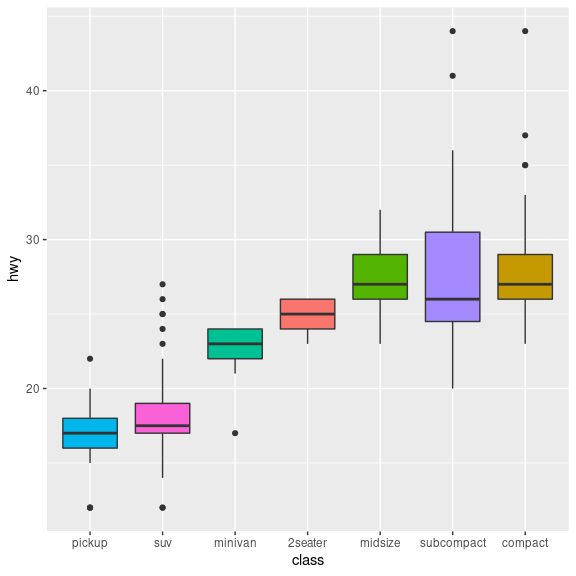
\includegraphics[width=2.08333in,height=\textheight]{images/rmarkdown/000002.png}
\caption{자동차 모델에 따른 고속도로 연비 분포}
\end{figure}

\begin{verbatim}
<center>
![자동차 모델에 따른 고속도로 연비 분포](images/rmarkdown/000002.png){width="200"}
</center>
\end{verbatim}

\begin{enumerate}
\def\labelenumi{\arabic{enumi}.}
\tightlist
\item
  첫 번째
\item
  두 번째
\item
  세 번째
\end{enumerate}

\begin{itemize}
\tightlist
\item
  아이템 1
\item
  아이템 2
\item
  아이템 3

  \begin{itemize}
  \tightlist
  \item
    아이템 3-1
  \item
    아이템 3-2
  \end{itemize}
\end{itemize}

\begin{verbatim}
1.  첫 번째
2.  두 번째
3.  세 번째

-   아이템 1
-   아이템 2
-   아이템 3
    -   아이템 3-1
    -   아이템 3-2
\end{verbatim}

참고로 소스코드 그대로 표현하기 위해서는 \texttt{\textasciitilde{}\textasciitilde{}\textasciitilde{}} 를 사용합니다.

\hypertarget{uxc2a4uxd0c0uxc77c}{%
\section{스타일}\label{uxc2a4uxd0c0uxc77c}}

아래와 같이 코드청크를 이용해서 css 코드를 삽입하고 해당되는 class 또는 id에 해당하는 내용에 스타일을 적용할 수 있습니다.

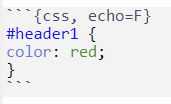
\includegraphics[width=1.5625in,height=\textheight]{images/02/style.png}

\leavevmode\vadjust pre{\hypertarget{header1}{}}%
소스코드

\begin{verbatim}
<div id='header1'>
소스코드 
</div>
\end{verbatim}

\hypertarget{uxd14cuxc774uxbe14}{%
\section{테이블}\label{uxd14cuxc774uxbe14}}

\texttt{kable} 함수를 이용하여 Rmarkdown 문서에 포함되는 표를 원하는 방향으로 작성할 수 있습니다. \texttt{mtcars}는 데이터프레임 형식의 데이터입니다.

\begin{Shaded}
\begin{Highlighting}[]
\NormalTok{knitr}\SpecialCharTok{::}\FunctionTok{kable}\NormalTok{(}
\NormalTok{  mtcars[}\DecValTok{1}\SpecialCharTok{:}\DecValTok{5}\NormalTok{, ], }
  \AttributeTok{caption =} \StringTok{"A knitr kable."}
\NormalTok{)}
\end{Highlighting}
\end{Shaded}

\begin{table}

\caption{\label{tab:unnamed-chunk-8}A knitr kable.}
\centering
\begin{tabular}[t]{l|r|r|r|r|r|r|r|r|r|r|r}
\hline
  & mpg & cyl & disp & hp & drat & wt & qsec & vs & am & gear & carb\\
\hline
Mazda RX4 & 21.0 & 6 & 160 & 110 & 3.90 & 2.620 & 16.46 & 0 & 1 & 4 & 4\\
\hline
Mazda RX4 Wag & 21.0 & 6 & 160 & 110 & 3.90 & 2.875 & 17.02 & 0 & 1 & 4 & 4\\
\hline
Datsun 710 & 22.8 & 4 & 108 & 93 & 3.85 & 2.320 & 18.61 & 1 & 1 & 4 & 1\\
\hline
Hornet 4 Drive & 21.4 & 6 & 258 & 110 & 3.08 & 3.215 & 19.44 & 1 & 0 & 3 & 1\\
\hline
Hornet Sportabout & 18.7 & 8 & 360 & 175 & 3.15 & 3.440 & 17.02 & 0 & 0 & 3 & 2\\
\hline
\end{tabular}
\end{table}

\hypertarget{yaml-uxd5e4uxb354}{%
\section{YAML 헤더}\label{yaml-uxd5e4uxb354}}

Rmarkdown 파일에서 YAML의 가장 중요한 기능은 output 포멧을 지정하는 것이며 title, author, date, 등을 설정할수도 있습니다.

\begin{verbatim}
---
layout: page
title: "R프로그래밍"
subtitle: "Rmarkdown 활용법"
output:
  html_document:
    css: style.css
    includes:
      in_header: header.html
      after_body: footer.html
    theme: default
    toc: yes
    toc_float: true
    highlight: tango
    code_folding: show
    number_sections: TRUE
mainfont: NanumGothic
---
\end{verbatim}

\hypertarget{output-format}{%
\section{Output format}\label{output-format}}

주요 문서 포멧으로 다음과 같은 몇 가지가 있습니다. 상세한 내용은 \href{https://rmarkdown.rstudio.com/lesson-9.html}{Rmarkdown output format}을 참고하시기 바랍니다.

\begin{itemize}
\tightlist
\item
  html\_document - HTML document w/ Bootstrap CSS
\item
  pdf\_document - PDF document (via LaTeX template)
\item
  word\_document - Microsoft Word document (docx)
\item
  ioslides\_presentation - HTML presentation with ioslides
\item
  beamer\_presentation - PDF presentation with LaTeX Beamer
\item
  powerpoint\_presentation: PowerPoint presentation
\end{itemize}

\textbf{Exercises}

``KRIBBR2022-Lecture2'' 라는 이름의 다음과 같은 형태의 Rmarkdown 문서를 만들고 이 번 강의의 실습 코드 및 설명, 질문, 코멘트 등을 적어 보시기 바랍니다.

\begin{center}\rule{0.5\linewidth}{0.5pt}\end{center}

이 저작물은 크리에이티브 커먼즈 저작자표시-비영리-변경금지 4.0 국제 라이선스에 따라 이용할 수 있습니다.

\hypertarget{r-programming}{%
\chapter{R programming}\label{r-programming}}

\hypertarget{console-calculator}{%
\section{Console calculator}\label{console-calculator}}

콘솔에서 바로 계산을 수행할 수 있습니다. 참고로 이전에 수행한 명령은 콘솔에 커서가 있는 상태에서 위 아래 화살표를 누르면 볼 수 있고 엔터를 눌러 재사용 할 수 있습니다. \texttt{;}을 사용하면 두 개의 명령을 동시에 수행할 수 있습니다.

\[ 2 + 2 \]
\[ ((2 - 1)^2 + (1 - 3)^2)^{1/2} \]

\begin{Shaded}
\begin{Highlighting}[]
\DecValTok{2} \SpecialCharTok{+} \DecValTok{2}
\NormalTok{((}\DecValTok{2}\NormalTok{ – }\DecValTok{1}\NormalTok{)}\SpecialCharTok{\^{}}\DecValTok{2} \SpecialCharTok{+}\NormalTok{ (}\DecValTok{1}\NormalTok{ – }\DecValTok{3}\NormalTok{)}\SpecialCharTok{\^{}}\DecValTok{2}\NormalTok{ )}\SpecialCharTok{\^{}}\NormalTok{(}\DecValTok{1}\SpecialCharTok{/}\DecValTok{2}\NormalTok{)}
\DecValTok{2} \SpecialCharTok{+} \DecValTok{2}\NormalTok{; }\DecValTok{2} \SpecialCharTok{{-}} \DecValTok{2}
\end{Highlighting}
\end{Shaded}

\textbf{Exercises}

다음 공식들을 계산하는 R 코드를 작성하시오

\[ \sqrt{(4+3)(2+1)} \]

\[ 2^3 + 3^2 \]

\[ \frac{0.25 - 0.2}{\sqrt{0.2 (1-0.2)/100}}\]

\hypertarget{what-is-a-programming-language}{%
\section{What is a programming language}\label{what-is-a-programming-language}}

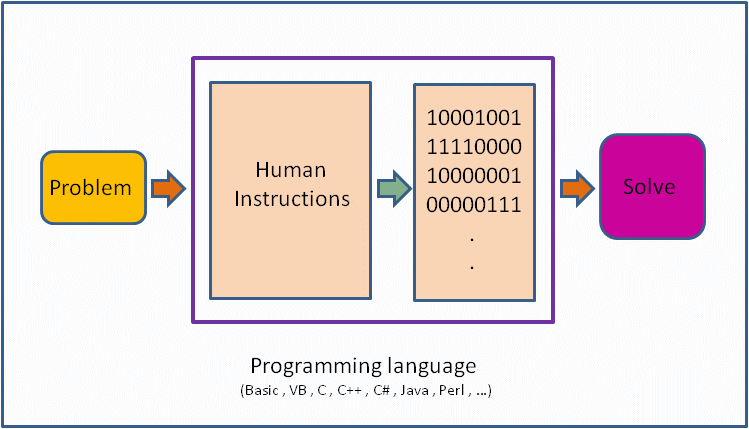
\includegraphics[width=4.16667in,height=\textheight]{images/01/24.PNG}

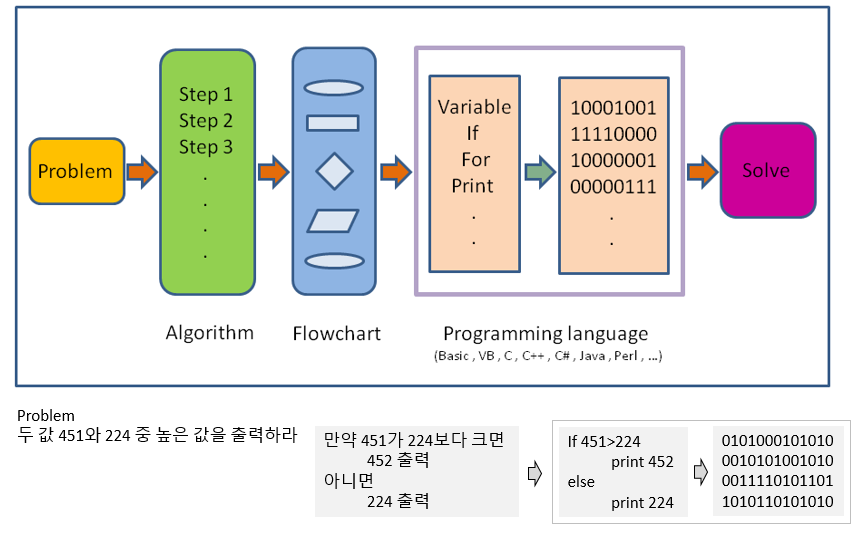
\includegraphics[width=4.375in,height=\textheight]{images/01/25.PNG}

R은 programming language로서 다른 프로그래밍 언어와 같이 몇 가지 공통적 개념을 가집니다 (\texttt{변수}, \texttt{자료형}, \texttt{함수}, \texttt{조건문}, \texttt{반복문})

\hypertarget{terminology}{%
\subsection{Terminology}\label{terminology}}

\begin{itemize}
\tightlist
\item
  Session: R 언어 실행 환경
\item
  Console: 명령어 입력하는 창
\item
  Code: R 프로그래밍 변수/제어문 모음
\item
  Object: 변수, 함수 등 프로그래밍에서 사용되는 모든 객체 (Data structure)

  \begin{itemize}
  \tightlist
  \item
    array: 1D, 2D, 3D, \ldots{} 형태 값들의 모임
  \item
    vector: 1차원 형태 값들의 모임 combine function \texttt{c()} EX: c(6, 11, 13, 31, 90, 92)
  \item
    matrix: 2차원 형태 값들의 모임 (같은 타입 값으로 구성)
  \item
    data frame: 2차원 형태 값들의 모임 (다른 타입 값 구성 가능)
  \item
    list: vector, matrix, data.frame 및 list 등 다양한 객체를 원소로 가집
  \end{itemize}
\item
  function: 특정 기능 수행, {[}함수이름, 입력값 (arguments), 출력값 (return){]} 으로 구성
\item
  Data (value): 값 - 자료형 (Data type)

  \begin{itemize}
  \tightlist
  \item
    Integers
  \item
    doubles/numerics
  \item
    logicals
  \item
    characters
  \item
    factor: 범주형
  \end{itemize}
\item
  Conditionals (조건, 제어):

  \begin{itemize}
  \tightlist
  \item
    \texttt{if}, \texttt{==}, \texttt{\&} (AND), \texttt{\textbar{}} (OR) Ex: \texttt{(2\ +\ 1\ ==\ 3)\ \&\ (2\ +\ 1\ ==\ 4)}
  \item
    \texttt{for}, \texttt{while}: 반복 수
  \end{itemize}
\end{itemize}

\hypertarget{data-and-variables}{%
\section{Data and variables}\label{data-and-variables}}

\hypertarget{data}{%
\subsection{Data}\label{data}}

일반적으로 데이터의 의미는 사실을 나타내는 수치입니다.

\begin{itemize}
\tightlist
\item
  맥도너 정보경제학 (1963)

  \begin{itemize}
  \tightlist
  \item
    지혜 (wisdom) : 패턴화된 지식
  \item
    지식 (knowledge) : 가치있는 정보
  \item
    정보 (information) : 의미있는 데이터
  \item
    데이터 (data) : 단순한 사실의 나열
  \end{itemize}
\end{itemize}

\begin{Shaded}
\begin{Highlighting}[]
\FunctionTok{library}\NormalTok{(UsingR)}
\NormalTok{exec.pay}
\NormalTok{?exec.pay}
\end{Highlighting}
\end{Shaded}

데이터는 속성에 따라서 다음과 같이 분류할 수 있습니다.

\begin{itemize}
\tightlist
\item
  범주형 - 질적 데이터, 숫자로 나타낼 수 있으나 의미 없음

  \begin{itemize}
  \tightlist
  \item
    명목형 (Nominal) - 사람 이름
  \item
    순서형 (Ordinal) -- 달리기 도착 순서
  \end{itemize}
\item
  수치형 - 숫자로 나타내며 데이터 속성을 그대로 지님님

  \begin{itemize}
  \tightlist
  \item
    구간형 (Interval) -- 선수1, 선수2 종점통과 시간
  \item
    비율형 (Ratio) -- 출발시간 기준 종점 통과 시간
  \end{itemize}
\end{itemize}

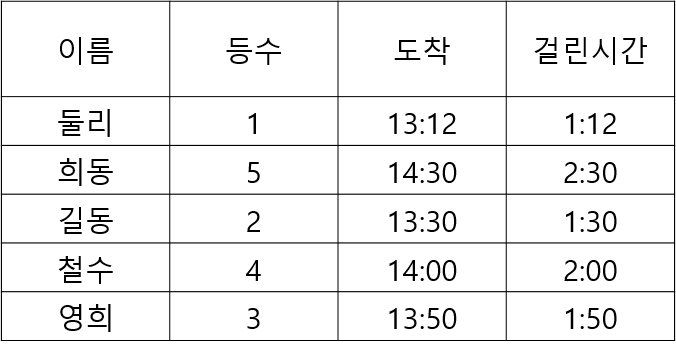
\includegraphics[width=3.125in,height=\textheight]{images/02/01.png}

\begin{itemize}
\tightlist
\item
  Data type in R

  \begin{itemize}
  \tightlist
  \item
    Numeric (수치형)

    \begin{itemize}
    \tightlist
    \item
      Discrete (이산형) data - 카운트, 횟수
    \item
      Continuous (연속형) data - 키, 몸무게, Cannot be shared
    \item
      Date and time
    \end{itemize}
  \item
    Factors (범주형)

    \begin{itemize}
    \tightlist
    \item
      Categories to group the data
    \item
      Character data - Identifiers (범주형)
    \end{itemize}
  \end{itemize}
\end{itemize}

\hypertarget{variables}{%
\subsection{Variables}\label{variables}}

변수는 데이터를 저장하는 공간으로 이해할 수 있습니다.

\begin{itemize}
\tightlist
\item
  Assignment operator ( \texttt{\textless{}-} OR \texttt{=} )

  \begin{itemize}
  \tightlist
  \item
    Valid object name \texttt{\textless{}-} value
  \item
    단축키: \texttt{Alt\ +\ -} (the minus sign)
  \end{itemize}
\item
  내장 변수 Built-in variables
\end{itemize}

\begin{Shaded}
\begin{Highlighting}[]
\NormalTok{x }\OtherTok{\textless{}{-}} \DecValTok{2}
\NormalTok{y }\OtherTok{\textless{}{-}}\NormalTok{ x}\SpecialCharTok{\^{}}\DecValTok{2}\NormalTok{ – }\DecValTok{2}\SpecialCharTok{*}\NormalTok{x }\SpecialCharTok{+} \DecValTok{1}
\NormalTok{y}
\NormalTok{x }\OtherTok{\textless{}{-}} \StringTok{"two"}  
\NormalTok{some\_data }\OtherTok{\textless{}{-}} \FloatTok{9.8}
\NormalTok{pi}
\end{Highlighting}
\end{Shaded}

\begin{itemize}
\tightlist
\item
  변수이름 작명법

  \begin{itemize}
  \tightlist
  \item
    Characters (letters), numbers, ``\_'', ``.''
  \item
    A and a are different symbols
  \item
    Names are effectively unlimited in length
  \end{itemize}
\end{itemize}

\begin{Shaded}
\begin{Highlighting}[]
\NormalTok{i\_use\_snake\_case }\OtherTok{\textless{}{-}} \DecValTok{1}
\NormalTok{otherPeopleUseCamelCase }\OtherTok{\textless{}{-}} \DecValTok{2}
\NormalTok{some.people.use.periods }\OtherTok{\textless{}{-}} \DecValTok{3}
\NormalTok{And\_aFew.People\_RENOUNCEconvention }\OtherTok{\textless{}{-}} \DecValTok{4}
\end{Highlighting}
\end{Shaded}

\hypertarget{object-data-structure}{%
\section{Object (Data structure)}\label{object-data-structure}}

변수, 함수 등 프로그래밍에서 사용되는 모든 개체를 말합니다.

\hypertarget{vector}{%
\subsection{vector}\label{vector}}

\texttt{vector}는 R의 기본 데이터 구조입니다. numeric vector, logical vector, character vector 등 저장되는 값의 타입에 따라 크게 세가지로 나눌 수 있습니다. \texttt{class()} 함수를 이용해서 값의 타입을 알아낼 수 있습니다. Combine function인 \texttt{c()}를 활용하여 만들며 값을 순차적으로 붙여갈 수 있습니다. 다음과 같은 Univariate (단변량, Single variable)을 표현할 때 사용됩니다.

\[ x_1, x_2, ..., x_n \]

\begin{Shaded}
\begin{Highlighting}[]
\NormalTok{x }\OtherTok{\textless{}{-}} \FunctionTok{c}\NormalTok{(}\FloatTok{10.4}\NormalTok{, }\FloatTok{5.6}\NormalTok{, }\FloatTok{3.1}\NormalTok{, }\FloatTok{6.4}\NormalTok{, }\FloatTok{21.7}\NormalTok{) }
\FunctionTok{class}\NormalTok{(x)}
\NormalTok{y }\OtherTok{\textless{}{-}} \FunctionTok{c}\NormalTok{(}\StringTok{"X1"}\NormalTok{, }\StringTok{"Y2"}\NormalTok{,  }\StringTok{"X3"}\NormalTok{,  }\StringTok{"Y4"}\NormalTok{)}
\FunctionTok{class}\NormalTok{(y)}
\NormalTok{z }\OtherTok{\textless{}{-}} \FunctionTok{c}\NormalTok{(T, F, F, T)}
\FunctionTok{class}\NormalTok{(z)}
\end{Highlighting}
\end{Shaded}

\hypertarget{numeric}{%
\subsubsection{numeric}\label{numeric}}

numeric 형식의 벡터는 다음과 같은 다양한 편의 함수들을 사용해서 만들수 있습니다.

\begin{Shaded}
\begin{Highlighting}[]
\DecValTok{1}\SpecialCharTok{:}\DecValTok{5}
\FunctionTok{seq}\NormalTok{(}\DecValTok{1}\NormalTok{,}\DecValTok{5}\NormalTok{, }\AttributeTok{by=}\DecValTok{1}\NormalTok{)}
\FunctionTok{seq}\NormalTok{(}\DecValTok{0}\NormalTok{, }\DecValTok{100}\NormalTok{, }\AttributeTok{by=}\DecValTok{10}\NormalTok{)}
\FunctionTok{seq}\NormalTok{(}\DecValTok{0}\NormalTok{, }\DecValTok{100}\NormalTok{, }\AttributeTok{length.out=}\DecValTok{11}\NormalTok{)}
\NormalTok{?seq}

\FunctionTok{rep}\NormalTok{(}\DecValTok{5}\NormalTok{, }\AttributeTok{times=}\DecValTok{10}\NormalTok{)}
\FunctionTok{rep}\NormalTok{(}\DecValTok{1}\SpecialCharTok{:}\DecValTok{3}\NormalTok{, }\AttributeTok{times=}\DecValTok{4}\NormalTok{)}
\FunctionTok{rep}\NormalTok{(}\DecValTok{1}\SpecialCharTok{:}\DecValTok{3}\NormalTok{, }\AttributeTok{each=}\DecValTok{3}\NormalTok{)}
\end{Highlighting}
\end{Shaded}

\textbf{Exercises}

odds라는 이름의 변수에 1부터 100까지의 홀수만을 저장하시오 (\texttt{seq()} 함수 사용)

인덱싱은 배열형 (vector, matrix 등) 데이터의 일부 데이터를 참조할 때 사용하는 방법입니다. \texttt{{[}}와 \texttt{{]}}를 사용하며 위치를 나타내는 수로 참조합니다.

\begin{Shaded}
\begin{Highlighting}[]
\NormalTok{x[}\DecValTok{1}\NormalTok{]}
\NormalTok{x[}\DecValTok{1}\SpecialCharTok{:}\DecValTok{3}\NormalTok{]}
\NormalTok{i }\OtherTok{\textless{}{-}} \DecValTok{1}\SpecialCharTok{:}\DecValTok{3}
\NormalTok{x[i]}
\NormalTok{x[}\FunctionTok{c}\NormalTok{(}\DecValTok{1}\NormalTok{,}\DecValTok{2}\NormalTok{,}\DecValTok{4}\NormalTok{)]}
\NormalTok{y[}\DecValTok{3}\NormalTok{]}
\end{Highlighting}
\end{Shaded}

또한 해당 위치의 이름으로 참조하기도 합니다.

\begin{Shaded}
\begin{Highlighting}[]
\FunctionTok{head}\NormalTok{(precip)}
\NormalTok{precip[}\DecValTok{1}\NormalTok{]}
\NormalTok{precip[}\DecValTok{2}\SpecialCharTok{:}\DecValTok{10}\NormalTok{]}
\NormalTok{precip[}\FunctionTok{c}\NormalTok{(}\DecValTok{1}\NormalTok{,}\DecValTok{3}\NormalTok{,}\DecValTok{5}\NormalTok{)]}
\NormalTok{precip[}\SpecialCharTok{{-}}\DecValTok{1}\NormalTok{]}
\NormalTok{precip[}\StringTok{"Seattle Tacoma"}\NormalTok{]}
\NormalTok{precip[}\FunctionTok{c}\NormalTok{(}\StringTok{"Seattle Tacoma"}\NormalTok{, }\StringTok{"Portland"}\NormalTok{)]}
\NormalTok{precip[}\DecValTok{2}\NormalTok{] }\OtherTok{\textless{}{-}} \DecValTok{10}
\end{Highlighting}
\end{Shaded}

참고로 vector 들은 다음과 같은 builtin 함수들을 사용해서 해당 변수의 attribute를 알아낼 수 있습니다. attribute에는 원소 이름, 타입, 길이 등 vector형 변수가 가질 수 있는 특성을 말합니다.

\begin{Shaded}
\begin{Highlighting}[]
\FunctionTok{head}\NormalTok{(precip)}
\FunctionTok{class}\NormalTok{(precip)}
\FunctionTok{length}\NormalTok{(precip)}
\FunctionTok{names}\NormalTok{(precip)}

\NormalTok{test\_scores }\OtherTok{\textless{}{-}} \FunctionTok{c}\NormalTok{(}\DecValTok{100}\NormalTok{, }\DecValTok{90}\NormalTok{, }\DecValTok{80}\NormalTok{)}
\FunctionTok{names}\NormalTok{(test\_scores) }\OtherTok{\textless{}{-}} \FunctionTok{c}\NormalTok{(}\StringTok{"Alice"}\NormalTok{, }\StringTok{"Bob"}\NormalTok{, }\StringTok{"Shirley"}\NormalTok{)}
\NormalTok{test\_scores}
\end{Highlighting}
\end{Shaded}

\hypertarget{logical}{%
\subsubsection{logical}\label{logical}}

Logical 벡터는 \texttt{True} 또는 \texttt{False}를 원소로 갖는 벡터 입니다. 앞글자가 대분자로 시작하는 것을 기억하시고 \texttt{T} 또는 \texttt{F}와 같이 한 문자로 표현할 수도 있습니다. 특정 조건에 대한 판단 결과를 반환할 경우에도 논리값을 사용합니다. 이 경우 조건을 판단 후 인덱싱 방법으로 (\texttt{which}, \texttt{any}, \texttt{all} 등 사용) 해당 값들을 뽑아내기도 합니다. 또한 활용이 많은 \texttt{sample} 함수의 사용법을 익혀둡니다.

\begin{Shaded}
\begin{Highlighting}[]
\NormalTok{x }\OtherTok{\textless{}{-}} \DecValTok{1}\SpecialCharTok{:}\DecValTok{20}
\NormalTok{x }\SpecialCharTok{\textgreater{}} \DecValTok{13}
\NormalTok{temp }\OtherTok{\textless{}{-}}\NormalTok{ x }\SpecialCharTok{\textgreater{}} \DecValTok{13}
\FunctionTok{class}\NormalTok{(temp)}

\NormalTok{ages }\OtherTok{\textless{}{-}} \FunctionTok{c}\NormalTok{(}\DecValTok{66}\NormalTok{, }\DecValTok{57}\NormalTok{, }\DecValTok{60}\NormalTok{, }\DecValTok{41}\NormalTok{,  }\DecValTok{6}\NormalTok{, }\DecValTok{85}\NormalTok{, }\DecValTok{48}\NormalTok{, }\DecValTok{34}\NormalTok{, }\DecValTok{61}\NormalTok{, }\DecValTok{12}\NormalTok{)}
\NormalTok{ages }\SpecialCharTok{\textless{}} \DecValTok{30}
\FunctionTok{which}\NormalTok{(ages }\SpecialCharTok{\textless{}} \DecValTok{30}\NormalTok{)}
\NormalTok{i }\OtherTok{\textless{}{-}} \FunctionTok{which}\NormalTok{(ages }\SpecialCharTok{\textless{}} \DecValTok{30}\NormalTok{)}
\NormalTok{ages[i]}
\FunctionTok{any}\NormalTok{(ages }\SpecialCharTok{\textless{}} \DecValTok{30}\NormalTok{)}
\FunctionTok{all}\NormalTok{(ages }\SpecialCharTok{\textless{}} \DecValTok{30}\NormalTok{)}

\NormalTok{random\_number }\OtherTok{\textless{}{-}} \FunctionTok{sample}\NormalTok{(}\FunctionTok{c}\NormalTok{(}\DecValTok{1}\SpecialCharTok{:}\DecValTok{10}\NormalTok{), }\DecValTok{2}\NormalTok{)}
\end{Highlighting}
\end{Shaded}

\textbf{Exercises}
1. 1부터 100까지의 수를 evens이라는 이름의 변수에 저장하고 이 중 짝수만을 뽑아내서 출력하시오 (\texttt{which()}함수 사용)

\begin{enumerate}
\def\labelenumi{\arabic{enumi}.}
\setcounter{enumi}{1}
\item
  \texttt{sample} 함수를 사용하여 앞서 odds와 evens 변수에서 랜덤하게 1개씩의 샘플을 뽑아서 \texttt{mynumbers}에 저장하시오
\item
  어떤 짝수가 뽑혔는지 찾아서 출력하시오 (\texttt{which}와 인덱싱 사용)
\end{enumerate}

\hypertarget{character}{%
\subsubsection{character}\label{character}}

Character(문자형) 벡터의 경우 문자열을 다루는데 자주 쓰이는 \texttt{paste()} 함수의 사용법을 알아두면 편리합니다. \texttt{paste()} 함수는 서로 다른 문자열을 붙이는데 주로 사용됩니다. 참고로 문자열을 나누는 함수는 \texttt{strsplit()} 입니다. \texttt{paste()}에서 붙이는 문자 사이에 들어가는 문자를 지정하는 파라메터는 \texttt{sep} 이고 \texttt{strsplit()}함수에서 자르는 기준이 되는 문자는\texttt{split} 파라미터로 지정해 줍니다 (\texttt{?split} 또는 \texttt{?paste} 확인).

\begin{Shaded}
\begin{Highlighting}[]
\FunctionTok{paste}\NormalTok{(}\StringTok{"X"}\NormalTok{, }\StringTok{"Y"}\NormalTok{, }\StringTok{"Z"}\NormalTok{, }\AttributeTok{sep=}\StringTok{"\_"}\NormalTok{)}
\FunctionTok{paste}\NormalTok{(}\FunctionTok{c}\NormalTok{(}\StringTok{"Four"}\NormalTok{,}\StringTok{"The"}\NormalTok{), }\FunctionTok{c}\NormalTok{(}\StringTok{"Score"}\NormalTok{,}\StringTok{"quick"}\NormalTok{), }\FunctionTok{c}\NormalTok{(}\StringTok{"and"}\NormalTok{,}\StringTok{"fox"}\NormalTok{), }\AttributeTok{sep=}\StringTok{"\_"}\NormalTok{)}
\FunctionTok{paste}\NormalTok{(}\StringTok{"X"}\NormalTok{, }\DecValTok{1}\SpecialCharTok{:}\DecValTok{5}\NormalTok{, }\AttributeTok{sep=}\StringTok{""}\NormalTok{)}
\FunctionTok{paste}\NormalTok{(}\FunctionTok{c}\NormalTok{(}\StringTok{"X"}\NormalTok{,}\StringTok{"Y"}\NormalTok{), }\DecValTok{1}\SpecialCharTok{:}\DecValTok{10}\NormalTok{, }\AttributeTok{sep=}\StringTok{""}\NormalTok{)}

\NormalTok{x }\OtherTok{\textless{}{-}} \FunctionTok{c}\NormalTok{(}\StringTok{"X1"}\NormalTok{, }\StringTok{"Y2"}\NormalTok{, }\StringTok{"X3"}\NormalTok{, }\StringTok{"Y4"}\NormalTok{, }\StringTok{"X5"}\NormalTok{)}
\FunctionTok{paste}\NormalTok{(x[}\DecValTok{1}\NormalTok{], x[}\DecValTok{2}\NormalTok{])}
\FunctionTok{paste}\NormalTok{(x[}\DecValTok{1}\NormalTok{], x[}\DecValTok{2}\NormalTok{], }\AttributeTok{sep=}\StringTok{""}\NormalTok{)}
\FunctionTok{paste}\NormalTok{(x, }\AttributeTok{collapse=}\StringTok{"\_"}\NormalTok{)}

\FunctionTok{strsplit}\NormalTok{(}\StringTok{"XYZ"}\NormalTok{, }\AttributeTok{split=}\StringTok{""}\NormalTok{)}
\FunctionTok{sort}\NormalTok{(}\FunctionTok{c}\NormalTok{(}\StringTok{"B"}\NormalTok{, }\StringTok{"C"}\NormalTok{, }\StringTok{"A"}\NormalTok{, }\StringTok{"D"}\NormalTok{))}
\end{Highlighting}
\end{Shaded}

\textbf{Exercises}

\begin{enumerate}
\def\labelenumi{\arabic{enumi}.}
\item
  \texttt{m}이라는 변수에 ``Capital of South Korea is Seoul'' 문자열을 저장하고 ``Capital of South Korea''를 따로 뽑아내 \texttt{m2}에 저장하시오 (\texttt{substr()} 사용)
\item
  \texttt{LETTERS} 내장함수에서 랜덤하게 10개의 문자를 뽑아내 myletters 변수에 저장하고 이들을 연결하여 (\texttt{paste} 사용) 하나의 문장(String)을 만드시오
\item
  myletters 변수의 문자들을 알파벳 순서대로 정렬하고 (\texttt{sort} 사용) 이들을 연결하여 하나의 문장 (String)을 만드시오
\end{enumerate}

\hypertarget{factor}{%
\subsubsection{factor}\label{factor}}

Factor형은 범주형데이터를 저장하기 위한 object 이며 R 언어에서 특별히 만들어져 사용되고 있습니다. \texttt{factor()} 함수를 이용해 생성하며 생성된 객체는 다음과 같이 \texttt{level}이라는 범주를 나타내는 특성값을 가지고 있습니다.

예를 들어 어린이 5명이 각각 빨강, 파랑, 노랑, 빨강, 파랑 색종이를 들고 있을때 색의 종류를 나타내는 값들은 빨강, 파랑, 노랑 입니다. 다섯 명의 아이들이 어떤 색의 색종이를 들고 있는지와는 상관없이 세 가지 범주의 값을 가지는 것 입니다.

\begin{Shaded}
\begin{Highlighting}[]
\NormalTok{x }\OtherTok{\textless{}{-}} \FunctionTok{c}\NormalTok{(}\StringTok{"Red"}\NormalTok{, }\StringTok{"Blue"}\NormalTok{, }\StringTok{"Yellow"}\NormalTok{, }\StringTok{"Red"}\NormalTok{, }\StringTok{"Blue"}\NormalTok{)}
\NormalTok{y }\OtherTok{\textless{}{-}} \FunctionTok{factor}\NormalTok{(x)}
\NormalTok{y}
\end{Highlighting}
\end{Shaded}

새로운 범주의 데이터를 추가할 경우 다음과 같이 해당되는 level을 먼저 추가하고 값을 저장해야 합니다.

\begin{Shaded}
\begin{Highlighting}[]
\FunctionTok{levels}\NormalTok{(y)}
\NormalTok{y[}\DecValTok{1}\NormalTok{] }\OtherTok{\textless{}{-}} \StringTok{"Gold"}
\NormalTok{y}

\FunctionTok{levels}\NormalTok{(y) }\OtherTok{\textless{}{-}} \FunctionTok{c}\NormalTok{(}\FunctionTok{levels}\NormalTok{(y), }\StringTok{"Gold"}\NormalTok{)}
\FunctionTok{levels}\NormalTok{(y)}
\NormalTok{y}
\NormalTok{y[}\DecValTok{1}\NormalTok{] }\OtherTok{\textless{}{-}} \StringTok{"Gold"}
\NormalTok{y}
\end{Highlighting}
\end{Shaded}

\texttt{factor}는 기본적으로 \texttt{level}에 표시된 순서가 위치 (정렬) 순서입니다. 이를 바꾸기 위해서는 다음과 같이 \texttt{levels} 함수를 이용해서 순서를 바꿀 수 있습니다.

\begin{Shaded}
\begin{Highlighting}[]
\FunctionTok{library}\NormalTok{(MASS)}
\FunctionTok{str}\NormalTok{(Cars93)}
\NormalTok{x }\OtherTok{\textless{}{-}}\NormalTok{ Cars93}\SpecialCharTok{$}\NormalTok{Origin}
\FunctionTok{plot}\NormalTok{(x)}
\FunctionTok{levels}\NormalTok{(x) }\OtherTok{\textless{}{-}} \FunctionTok{c}\NormalTok{(}\StringTok{"non{-}USA"}\NormalTok{, }\StringTok{"USA"}\NormalTok{)}
\FunctionTok{levels}\NormalTok{(x)}
\FunctionTok{plot}\NormalTok{(x)}
\end{Highlighting}
\end{Shaded}

::: rmdnote
\textbf{Exercises}

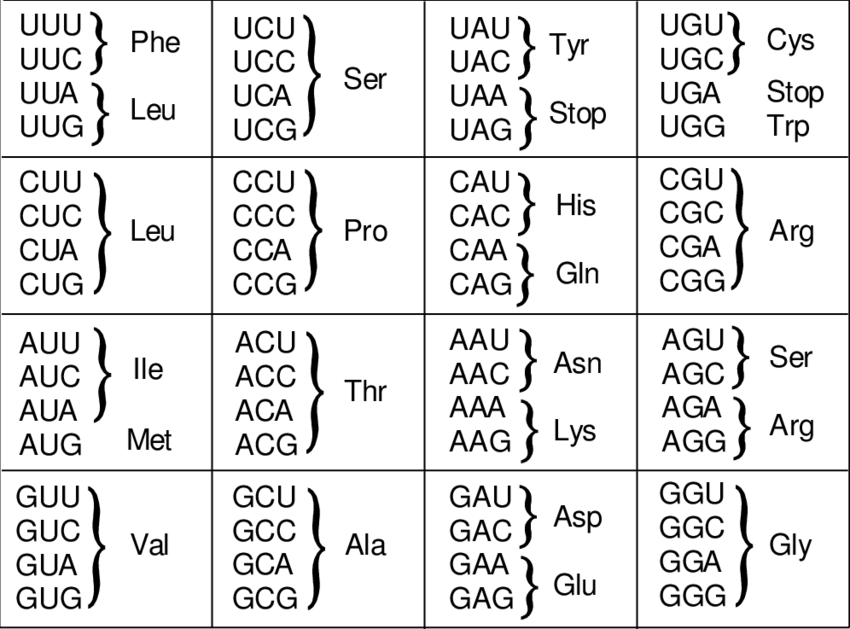
\includegraphics[width=3.64583in,height=\textheight]{images/03/codon_table.png}
1. 아미노산 Phe, Leu, Ser 를 값으로 갖는 범주형 변수 (factor)를 생성하시오
2. 각 아미노산과 해당 아미노산을 코딩하는 nucleotide triplets (codon)을 어떤 형태의 변수로 저장할 수 있을지 고민해 보시오

:::

\hypertarget{missing-values}{%
\subsubsection{Missing values}\label{missing-values}}

특정 값이 ``Not available'' 이거나 ``Missing value'' 일 경우 벡터의 해당 원소 자리에 데이터의 이상을 알리기 위해 \texttt{NA}를 사용합니다. 따라서 일반적인 연산에서 \texttt{NA}가 포함되어 있는 경우 데이터의 불완전성을 알리기 위해 연산의 결과는 \texttt{NA}가 됩니다. \texttt{is.na()} 함수는 해당 변수에 \texttt{NA} 값이 있는지를 검사해주는 함수이며 R에는 이 외에도 다음과 같은 특수 값들이 사용되고 있습니다.

\begin{itemize}
\tightlist
\item
  NA: Not available, The value is missing
\item
  NULL: a reserved value
\item
  NaN: Not a number (0/0)
\item
  Inf: (1/0)
\end{itemize}

\begin{Shaded}
\begin{Highlighting}[]
\NormalTok{hip\_cost }\OtherTok{\textless{}{-}} \FunctionTok{c}\NormalTok{(}\DecValTok{10500}\NormalTok{, }\DecValTok{45000}\NormalTok{, }\DecValTok{74100}\NormalTok{, }\ConstantTok{NA}\NormalTok{, }\DecValTok{83500}\NormalTok{)}
\FunctionTok{sum}\NormalTok{(hip\_cost)}
\FunctionTok{sum}\NormalTok{(hip\_cost, }\AttributeTok{na.rm=}\ConstantTok{TRUE}\NormalTok{)}
\NormalTok{?sum}
\end{Highlighting}
\end{Shaded}

\hypertarget{useful-functions}{%
\subsubsection{Useful functions}\label{useful-functions}}

다음은 벡터형 변수와 같이 쓰이는 유용한 함수들입니다.

\begin{Shaded}
\begin{Highlighting}[]
\NormalTok{z }\OtherTok{\textless{}{-}} \FunctionTok{sample}\NormalTok{(}\DecValTok{1}\SpecialCharTok{:}\DecValTok{10}\NormalTok{, }\DecValTok{100}\NormalTok{, T)}
\FunctionTok{head}\NormalTok{(z)}
\FunctionTok{sort}\NormalTok{(z)}
\FunctionTok{order}\NormalTok{(z)}
\FunctionTok{table}\NormalTok{(z)}
\NormalTok{p }\OtherTok{\textless{}{-}}\NormalTok{ z}\SpecialCharTok{/}\FunctionTok{sum}\NormalTok{(z)}
\FunctionTok{round}\NormalTok{(p, }\AttributeTok{digits=}\DecValTok{1}\NormalTok{)}
\end{Highlighting}
\end{Shaded}

\texttt{is} 함수를 사용하여 데이터 타입이 사용자가 의도한 타입과 맞는지 검사할 수 있습니다. 콘솔창에서 \texttt{is.}를 타이핑한 후 잠시 기다리면 다양한 is 합수를 볼 수 있습니다.

\begin{Shaded}
\begin{Highlighting}[]
\FunctionTok{is.na}\NormalTok{(}\DecValTok{1}\NormalTok{)}
\FunctionTok{is.numeric}\NormalTok{(}\DecValTok{1}\NormalTok{)}
\FunctionTok{is.logical}\NormalTok{(}\ConstantTok{TRUE}\NormalTok{)}
\FunctionTok{is.data.frame}\NormalTok{(}\StringTok{"A"}\NormalTok{)}
\FunctionTok{is.character}\NormalTok{(}\StringTok{"A"}\NormalTok{)}
\end{Highlighting}
\end{Shaded}

\texttt{as} 함수는 데이터 타입을 변환해주는 함수입니다.

\begin{Shaded}
\begin{Highlighting}[]
\NormalTok{digits }\OtherTok{\textless{}{-}} \FunctionTok{runif}\NormalTok{(}\DecValTok{10}\NormalTok{)}\SpecialCharTok{*}\DecValTok{10}
\FunctionTok{class}\NormalTok{(digits)}
\NormalTok{digits\_int }\OtherTok{\textless{}{-}} \FunctionTok{as.integer}\NormalTok{(digits)}
\FunctionTok{class}\NormalTok{(digits\_int)}
\NormalTok{digits\_char }\OtherTok{\textless{}{-}} \FunctionTok{as.character}\NormalTok{(digits\_int)}
\FunctionTok{class}\NormalTok{(digits\_char)}
\NormalTok{digits\_num }\OtherTok{\textless{}{-}} \FunctionTok{as.numeric}\NormalTok{(digits\_char)}
\FunctionTok{class}\NormalTok{(digits\_num)}
\end{Highlighting}
\end{Shaded}

\hypertarget{matrix}{%
\subsection{matrix}\label{matrix}}

매트릭스는 2차원 행렬로 같은 형식의 데이터 값 (numberic, character, logical) 으로만 채워진 행렬을 말합니다. 메트릭스를 만드는 방법은 아래와 같으며 \texttt{nrow} 와 \texttt{ncol} 파라메터에 행과 열의 수를 넣고 각 셀에 들어갈 값은 가장 앞에 위치한 data 파라메터에 넣어 줍니다 (\texttt{?matrix}로 파라메터 이름 확인). 메트릭스 인덱싱은 메트릭스 안의 값을 저장하거나 참조할때 (빼올때) 사용하는 방법입니다. 메트릭스 변수이름 바로 뒤에 대괄호를 이용해서 제어를 하며 대괄호 안에 콤마로 구분된 앞쪽은 row, 뒷쪽은 column 인덱스를 나타냅니다.

\begin{Shaded}
\begin{Highlighting}[]
\NormalTok{mymat }\OtherTok{\textless{}{-}} \FunctionTok{matrix}\NormalTok{(}\DecValTok{0}\NormalTok{, }\AttributeTok{nrow=}\DecValTok{100}\NormalTok{, }\AttributeTok{ncol=}\DecValTok{3}\NormalTok{) }\CommentTok{\# 1}
\NormalTok{mymat[,}\DecValTok{1}\NormalTok{] }\OtherTok{\textless{}{-}} \DecValTok{1}\SpecialCharTok{:}\DecValTok{100} \CommentTok{\# 2}
\NormalTok{mymat[,}\DecValTok{2}\NormalTok{] }\OtherTok{\textless{}{-}} \FunctionTok{seq}\NormalTok{(}\DecValTok{1}\NormalTok{,}\DecValTok{200}\NormalTok{,}\DecValTok{2}\NormalTok{) }\CommentTok{\# 3}
\NormalTok{mymat[,}\DecValTok{3}\NormalTok{] }\OtherTok{\textless{}{-}} \FunctionTok{seq}\NormalTok{(}\DecValTok{2}\NormalTok{,}\DecValTok{200}\NormalTok{,}\DecValTok{2}\NormalTok{) }\CommentTok{\# 4}
\end{Highlighting}
\end{Shaded}

매트릭스의 row나 column에 이름이 주어져 있을 경우 이름을 따옴표(``)로 묶은 후 참조가 가능합니다. row나 column의 이름은 \texttt{rownames()} 또는 \texttt{colnames()}로 생성하거나 변경할 수 있습니다. row나 column의 개수는 \texttt{nrow()} 또는 \texttt{ncol()} 함수를 사용합니다.

\begin{Shaded}
\begin{Highlighting}[]
\FunctionTok{colnames}\NormalTok{(mymat)}
\FunctionTok{colnames}\NormalTok{(mymat) }\OtherTok{\textless{}{-}} \FunctionTok{c}\NormalTok{(}\StringTok{"A"}\NormalTok{, }\StringTok{"B"}\NormalTok{, }\StringTok{"C"}\NormalTok{)}
\FunctionTok{colnames}\NormalTok{(mymat)}
\FunctionTok{colnames}\NormalTok{(mymat)[}\DecValTok{2}\NormalTok{] }\OtherTok{\textless{}{-}} \StringTok{"D"}
\FunctionTok{colnames}\NormalTok{(mymat)}
\FunctionTok{rownames}\NormalTok{(mymat) }\OtherTok{\textless{}{-}} \FunctionTok{paste}\NormalTok{(}\StringTok{"No"}\NormalTok{, }\DecValTok{1}\SpecialCharTok{:}\FunctionTok{nrow}\NormalTok{(mymat), }\AttributeTok{sep=}\StringTok{""}\NormalTok{)}
\FunctionTok{rownames}\NormalTok{(mymat)}
\end{Highlighting}
\end{Shaded}

여러 row나 column을 참조할 경우 아래와 같이 combine 함수를 사용하여 묶어줘야 하며 스칼라값을 (임의의 숫자 하나) 더하거나 뺄 경우 vector / matrix 연산을 기본으로 수행합니다.

\begin{Shaded}
\begin{Highlighting}[]
\NormalTok{mymat[}\FunctionTok{c}\NormalTok{(}\DecValTok{2}\NormalTok{,}\DecValTok{3}\NormalTok{,}\DecValTok{4}\NormalTok{,}\DecValTok{5}\NormalTok{),}\DecValTok{2}\NormalTok{] }\CommentTok{\# 5}
\NormalTok{mymat}\DecValTok{{-}1} \CommentTok{\# 6}
\NormalTok{mysub }\OtherTok{\textless{}{-}}\NormalTok{ mymat[,}\DecValTok{2}\NormalTok{] }\SpecialCharTok{{-}}\NormalTok{ mymat[,}\DecValTok{1}\NormalTok{] }\CommentTok{\#7}
\FunctionTok{sum}\NormalTok{(mysub) }\CommentTok{\#8}
\FunctionTok{sum}\NormalTok{(mysub}\SpecialCharTok{\^{}}\DecValTok{2}\NormalTok{) }\CommentTok{\#8}
\end{Highlighting}
\end{Shaded}

\textbf{Exercises}

\begin{enumerate}
\def\labelenumi{\arabic{enumi}.}
\tightlist
\item
  score 라는 변수에 1부터 100까지 중 랜덤하게 선택된 20개의 수로 10 x 2 matrix를 만드시오 (\texttt{sample()} 사용)
\item
  score의 row 이름을 문자형으로 Name1, Name2, \ldots, Name10으로 지정하시오 (\texttt{paste()} 사용)
\item
  score의 column 이름을 문자형으로 math와 eng로 지정하시오
\item
  이 matrix의 첫번째 컬럼과 두 번째 컬럼의 수를 각각 더한 후 \texttt{total\_score}라는 변수에 저장하시오
\item
  \texttt{total\_score}의의 오름차순 순서를 나타내는 인덱스 (\texttt{order()}함수 사용)를 \texttt{o}라는 변수에 저장하시오
\item
  score를 \texttt{o}순서로 재배치하고 score\_ordered 변수에 저장하시오
\end{enumerate}

\hypertarget{data.frame}{%
\subsection{data.frame}\label{data.frame}}

데이터프레임은 형태는 매트릭스와 같으나 컬럼 하나가 하나의 vector형 변수로서 각 변수들이 다른 모드의 값을 저장할 수 있다는 차이가 있습니다. \texttt{\$} 기호를 이용하여 각 구성 변수를 참조할 수 있습니다. 컬럼 한 줄이 하나의 변수 이므로 새로운 변수도 컬럼 형태로 붙여 넣을 수 있습니다. 즉, 각 row는 샘플을 나타내고 각 column은 변수를 나타내며 각 변수들이 갖는 샘플의 개수 (row의 길이, vector 의 길이)는 같아야 합니다. R 기반의 데이터 분석에서는 가장 선호되는 데이터 타입이라고 볼 수 있습니다.

\begin{Shaded}
\begin{Highlighting}[]
\DocumentationTok{\#\# data.frame}
\NormalTok{ids }\OtherTok{\textless{}{-}} \DecValTok{1}\SpecialCharTok{:}\DecValTok{10}
\NormalTok{ids}
\NormalTok{idnames }\OtherTok{\textless{}{-}} \FunctionTok{paste}\NormalTok{(}\StringTok{"Name"}\NormalTok{, ids, }\AttributeTok{sep=}\StringTok{""}\NormalTok{)}
\NormalTok{idnames}
\NormalTok{students }\OtherTok{\textless{}{-}} \FunctionTok{data.frame}\NormalTok{(ids, idnames)}
\NormalTok{students}
\FunctionTok{class}\NormalTok{(students}\SpecialCharTok{$}\NormalTok{ids)}
\FunctionTok{class}\NormalTok{(students}\SpecialCharTok{$}\NormalTok{idnames)}
\NormalTok{students}\SpecialCharTok{$}\NormalTok{idnames}
\FunctionTok{str}\NormalTok{(students)}

\NormalTok{students }\OtherTok{\textless{}{-}} \FunctionTok{data.frame}\NormalTok{(ids, idnames, }\AttributeTok{stringsAsFactors =}\NormalTok{ F)}
\FunctionTok{class}\NormalTok{(students}\SpecialCharTok{$}\NormalTok{idnames)}
\NormalTok{students}\SpecialCharTok{$}\NormalTok{idnames}
\NormalTok{students[}\DecValTok{1}\NormalTok{,]}
\FunctionTok{str}\NormalTok{(students)}
\end{Highlighting}
\end{Shaded}

데이터프레임에서는 \texttt{\$}를 사용하여 변수 이름으로 인덱싱이 가능합니다.

\begin{Shaded}
\begin{Highlighting}[]
\DocumentationTok{\#\# data frame indexing }
\NormalTok{students}\SpecialCharTok{$}\NormalTok{ids}
\NormalTok{students[,}\DecValTok{1}\NormalTok{]}
\NormalTok{students[,}\StringTok{"ids"}\NormalTok{]}
\end{Highlighting}
\end{Shaded}

\textbf{Exercises}

\begin{enumerate}
\def\labelenumi{\arabic{enumi}.}
\tightlist
\item
  \texttt{math}라는 변수에 1부터 100까지 중 랜덤하게 선택된 10개의 수를 넣으시오
\item
  \texttt{eng}라는 변수에 1부터 100까지 중 랜덤하게 선택된 10개의 수를 넣으시오
\item
  \texttt{students}라는 변수에 문자형으로 Name1, Name2, \ldots, Name10으로 지정하시오 (\texttt{paste()} 사용)
\item
  \texttt{math}와 \texttt{eng}라는 벡터에 저장된 값들의 이름을 \texttt{students} 변수에 저장된 이름으로 지정하시오
\item
  \texttt{math}와 \texttt{eng} 벡터를 갖는 \texttt{score} 라는 \texttt{data.frame}을 만드시오
\item
  \texttt{math}와 \texttt{eng} 변수를 지우시오 (\texttt{rm()}사용)
\item
  \texttt{score} data frame의 \texttt{math}와 \texttt{eng}를 각각 더한 후 \texttt{total\_score}라는 변수에 저장 하시오
\end{enumerate}

\hypertarget{list}{%
\subsection{list}\label{list}}

리스트는 변수들의 모임이라는 점에서 데이터프레임과 같으나 구성 변수들의 길이가 모두 같아야 하는 데이터프레임과는 달리 다른 길이의 변수를 모아둘 수 있는 점이 다릅니다. 즉, R언어에서 두 변수를 담을 수 있는 데이터 타입은 \texttt{list}와 \texttt{data\ frame} 두 종류가 있는데 \texttt{list} 변수 타입은 \texttt{vector} 형태의 여러개의 element를 가질 수 있으며 각 \texttt{vector의} 길이가 모두 달라도 됩니다. list의 인덱싱에서 \texttt{{[}} \texttt{{]}}는 리스트를 반환하고 \texttt{{[}{[}} \texttt{{]}{]}}는 vector element들을 반환합니다.

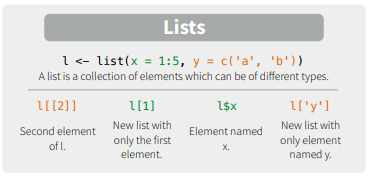
\includegraphics[width=3.125in,height=\textheight]{images/03/05.PNG}

\begin{Shaded}
\begin{Highlighting}[]
\DocumentationTok{\#\# list}
\NormalTok{parent\_names }\OtherTok{\textless{}{-}} \FunctionTok{c}\NormalTok{(}\StringTok{"Fred"}\NormalTok{, }\StringTok{"Mary"}\NormalTok{)}
\NormalTok{number\_of\_children }\OtherTok{\textless{}{-}} \DecValTok{2}
\NormalTok{child\_ages }\OtherTok{\textless{}{-}} \FunctionTok{c}\NormalTok{(}\DecValTok{4}\NormalTok{, }\DecValTok{7}\NormalTok{, }\DecValTok{9}\NormalTok{)}
\FunctionTok{data.frame}\NormalTok{(parent\_names, number\_of\_children, child\_ages)}
\NormalTok{lst }\OtherTok{\textless{}{-}} \FunctionTok{list}\NormalTok{(parent\_names, number\_of\_children, child\_ages)}
\NormalTok{lst[}\DecValTok{1}\NormalTok{]}
\NormalTok{lst[[}\DecValTok{1}\NormalTok{]]}
\FunctionTok{class}\NormalTok{(lst[}\DecValTok{1}\NormalTok{])}
\FunctionTok{class}\NormalTok{(lst[[}\DecValTok{1}\NormalTok{]])}
\NormalTok{lst[[}\DecValTok{1}\NormalTok{]][}\DecValTok{1}\NormalTok{]}
\NormalTok{lst[[}\DecValTok{1}\NormalTok{]][}\FunctionTok{c}\NormalTok{(}\DecValTok{1}\NormalTok{,}\DecValTok{2}\NormalTok{)]}
\end{Highlighting}
\end{Shaded}

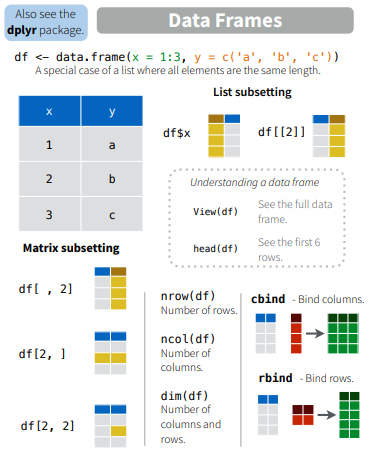
\includegraphics[width=2.60417in,height=\textheight]{images/03/06.PNG}

\textbf{Exercises}

\begin{enumerate}
\def\labelenumi{\arabic{enumi}.}
\item
  위 아미노산 예제에서 Phe, Leu, Ser 각각의 코돈을 원소로 갖는 세 개의 vector 변수들을 만들고 이를 \texttt{aalist} 라는 이름의 하나의 리스트 변수로 만드시오
\item
  \texttt{aalist} 리스트를 data.frame 형식의 \texttt{aadf} 변수로 만드시오 (데이터 구조를 바꾸어 저장 가능)
\end{enumerate}

\hypertarget{functions}{%
\section{Functions}\label{functions}}

함수(Function)란 사용자가 원하는 기능을 수행하는 코드의 모음으로서 반복적으로 쉽게 사용할 수 있도록 만들어 놓은 코드 입니다.

\hypertarget{a-script-in-r}{%
\subsection{A script in R}\label{a-script-in-r}}

함수의 개념을 배우기 전에 스크립트를 활용한 명령어 수행을 알아보겠습니다. R 프로그래밍을 통해서 사용자가 원하는 기능을 수행하는 방법은 다음과 같이 스크립트를 만들어서 실행하는 것 입니다. 일반적으로 R을 이용한 스크립트 명령을 어떻게 실행하는지 알아보겠습니다. 다음 예제는 입력 값들의 평균을 계산해서 출력해 주는 스크립트 명령입니다. R base 패키지에서 기본으로 제공되는 \texttt{mean()}이라는 함수가 있지만 사용하지 않고 \texttt{sum()}과 \texttt{length()} 함수를 사용했습니다.

\begin{Shaded}
\begin{Highlighting}[]

\NormalTok{numbers }\OtherTok{\textless{}{-}} \FunctionTok{c}\NormalTok{(}\FloatTok{0.452}\NormalTok{, }\FloatTok{1.474}\NormalTok{, }\FloatTok{0.22}\NormalTok{, }\FloatTok{0.545}\NormalTok{, }\FloatTok{1.205}\NormalTok{, }\FloatTok{3.55}\NormalTok{)}
\FunctionTok{cat}\NormalTok{(}\StringTok{"Input numbers are"}\NormalTok{, numbers, }\StringTok{"}\SpecialCharTok{\textbackslash{}n}\StringTok{"}\NormalTok{)}
\NormalTok{numbers\_mean }\OtherTok{\textless{}{-}} \FunctionTok{sum}\NormalTok{(numbers)}\SpecialCharTok{/}\FunctionTok{length}\NormalTok{(numbers)}
\NormalTok{out }\OtherTok{\textless{}{-}} \FunctionTok{paste}\NormalTok{(}\StringTok{"The average is "}\NormalTok{, numbers\_mean, }\StringTok{".}\SpecialCharTok{\textbackslash{}n}\StringTok{"}\NormalTok{, }\AttributeTok{sep=}\StringTok{""}\NormalTok{)}
\FunctionTok{cat}\NormalTok{(out)}
\end{Highlighting}
\end{Shaded}

상황에 따라 다르긴 하지만 보통 위 스크립트를 실행할 때 R 파일을 하나 만들고 \texttt{source()}라는 함수를 사용해서 파일 전체를 한번에 읽어들이고 실행을 시킵니다. 위 코드를 \texttt{myscript.R} 이라는 새로운 R 파일을 하나 만들고 저장 후 다음과 같이 실행할 수 있습니다. 참고로 위 파일은 현재 Working directory와 같은 위치에 저장해야 합니다.

\begin{Shaded}
\begin{Highlighting}[]
\FunctionTok{source}\NormalTok{(}\StringTok{"myscript.R"}\NormalTok{)}
\end{Highlighting}
\end{Shaded}

그러나 위와 같은 식으로 실행할 경우 다음 몇 가지 문제가 있습니다. 하나는 입력 값이 바뀔 때마나 파일을 열어 바뀐 값을 저장해 줄 필요가 있습니다. 결과 값에 대해서 다른 처리를 하고 싶을 경우 또한 파일을 직접 수정해 주어야 합니다. 또한 모든 변수들이 전역변수로 사용되어 코드가 복잡해질 경우 변수간 간섭이 생길 가능성이 높습니다.

\hypertarget{build-a-function}{%
\subsection{Build a function}\label{build-a-function}}

함수는 특정 데이터를 입력으로 받아 원하는 기능을 수행한 후 결과 데이터를 반환하는 구조를 가집니다. 함수는 일반적으로 다음과 같은 포멧으로 구현할 수 있습니다.

\begin{Shaded}
\begin{Highlighting}[]
\NormalTok{my\_function\_name }\OtherTok{\textless{}{-}} \ControlFlowTok{function}\NormalTok{(parameter1, parameter2, ... )\{}
  \DocumentationTok{\#\#any statements}
  \FunctionTok{return}\NormalTok{(object)}
\NormalTok{\}}
\end{Highlighting}
\end{Shaded}

예를 들어 다음과 같은 \texttt{my\_sine} 함수를 만들 수 있으며 parameter (매개변수)는 \texttt{x}이고 \texttt{y}는 반환값을 저장하는 지역변수 입니다.

\begin{Shaded}
\begin{Highlighting}[]
\NormalTok{my\_sine }\OtherTok{\textless{}{-}} \ControlFlowTok{function}\NormalTok{(x)\{}
\NormalTok{    y }\OtherTok{\textless{}{-}} \FunctionTok{sin}\NormalTok{(x)}
    \FunctionTok{return}\NormalTok{(y)}
\NormalTok{\}}
\end{Highlighting}
\end{Shaded}

만들어진 함수는 다음과 같이 사용할 수 있습니다. 만들어진 함수는 처음에 한 번 실행해 주어 실행중인 R session에 등록한 후 사용할 수 있습니다. 여기서 함수로 전달되는 값 \texttt{pi}는 argument (전달인자) 라고 합니다. 전달인자는 함수에서 정의된 매개변수의 갯수와 같은 수의 전달인자를 입력해 주어야 합니다. 참고로 parameter와 argument는 많은 사람들이 혼동하는 단어입니다. 본 예에서 \texttt{my\_sine}함수의 괄호 안에 있는 변수 \texttt{x}는 parameter이고 \texttt{x}에 들어가는 값인 \texttt{pi} 나 \texttt{90}은 argument 입니다.

\begin{Shaded}
\begin{Highlighting}[]
\FunctionTok{my\_sine}\NormalTok{(pi)}
\FunctionTok{my\_sine}\NormalTok{(}\DecValTok{90}\NormalTok{)}
\FunctionTok{sin}\NormalTok{(}\DecValTok{90}\NormalTok{)}
\end{Highlighting}
\end{Shaded}

\begin{itemize}
\item
  Terminology

  \begin{itemize}
  \tightlist
  \item
    function name: \texttt{my\_sine}
  \item
    parameter: \texttt{x}
  \item
    argument: \texttt{pi}
  \item
    return value: \texttt{y}
  \end{itemize}
\end{itemize}

이제 위 스크립트 (\texttt{myscript.R}) 에서 사용된 코드를 함수로 바꿔봅니다. numbers (전달인자)를 받는 매개변수를 x로 하고 함수 이름은 \texttt{mymean} 이고 평균값 (numbers\_mean)을 반환하는 합수입니다.

\begin{Shaded}
\begin{Highlighting}[]
\NormalTok{numbers }\OtherTok{\textless{}{-}} \FunctionTok{c}\NormalTok{(}\FloatTok{0.452}\NormalTok{, }\FloatTok{1.474}\NormalTok{, }\FloatTok{0.22}\NormalTok{, }\FloatTok{0.545}\NormalTok{, }\FloatTok{1.205}\NormalTok{, }\FloatTok{3.55}\NormalTok{)}

\NormalTok{mymean }\OtherTok{\textless{}{-}} \ControlFlowTok{function}\NormalTok{(x)\{}
  \FunctionTok{cat}\NormalTok{(}\StringTok{"Input numbers are"}\NormalTok{, x, }\StringTok{"}\SpecialCharTok{\textbackslash{}n}\StringTok{"}\NormalTok{)}
\NormalTok{  numbers\_mean }\OtherTok{\textless{}{-}} \FunctionTok{sum}\NormalTok{(x)}\SpecialCharTok{/}\FunctionTok{length}\NormalTok{(x)}
\NormalTok{  out }\OtherTok{\textless{}{-}} \FunctionTok{paste}\NormalTok{(}\StringTok{"The average is "}\NormalTok{, numbers\_mean, }\StringTok{".}\SpecialCharTok{\textbackslash{}n}\StringTok{"}\NormalTok{, }\AttributeTok{sep=}\StringTok{""}\NormalTok{)}
  \FunctionTok{cat}\NormalTok{(out)}
  \FunctionTok{return}\NormalTok{(numbers\_mean)}
\NormalTok{\}}

\NormalTok{retval }\OtherTok{\textless{}{-}} \FunctionTok{mymean}\NormalTok{(numbers)}
\FunctionTok{cat}\NormalTok{(retval)}
\end{Highlighting}
\end{Shaded}

\texttt{myscript.R}이라는 파일을 열고 작성된 스크립트에 더해서 아래처럼 함수 코드를 만들 경우 \texttt{source()} 함수로 함수를 세션으로 읽어오고 바로 사용할 수 있습니다. 위와 같이 함수를 만들 경우 입력 값을 언제든 바꿔서 사용할 수 있고 반환값에 대한 추가적인 연산도 쉽게 수행 할 수 있습니다.

\begin{Shaded}
\begin{Highlighting}[]
\NormalTok{new\_values }\OtherTok{\textless{}{-}} \FunctionTok{c}\NormalTok{(}\DecValTok{1}\SpecialCharTok{:}\DecValTok{10}\NormalTok{)}
\NormalTok{retval }\OtherTok{\textless{}{-}} \FunctionTok{mymean}\NormalTok{(new\_values)}
\NormalTok{retval}
\end{Highlighting}
\end{Shaded}

\textbf{Exercises}

\begin{enumerate}
\def\labelenumi{\arabic{enumi}.}
\item
  변수 \texttt{x}에 1, 3, 5, 7, 9를, 변수 \texttt{y}에 2, 4, 6, 8, 10을 저장하는 코드를 작성하시오
\item
  \texttt{x}와 \texttt{y}를 더한 값을 \texttt{z}에 저장하는 코드를 작성하시오
\item
  \texttt{mysum} 이라는 이름의 함수를 작성하되 두 변수를 입력으로 받아 더한 후 결과를 반환하는 코드를 작성하시오
\item
  \texttt{mymean} 이라는 이름의 함수를 작성하되 두 변수를 입력으로 받아 평균을 구한 후 결과를 반환하는 코드를 작성하시오
\end{enumerate}

\textbf{Exercises}

\begin{enumerate}
\def\labelenumi{\arabic{enumi})}
\tightlist
\item
  \texttt{mysd}라는 이름의 (표본)표준편차를 구하는 함수를 \texttt{myscript.R} 파일에 구현하시오 (\texttt{sd()}함수 사용하지 않고, 다음 표준편차 공식 이용)
\end{enumerate}

\[ 
\sigma = \sqrt{\frac{\sum(x-mean(x))^2}{length(x)-1}} 
\]

코드는 아래와 같음

\begin{Shaded}
\begin{Highlighting}[]
\NormalTok{mysd }\OtherTok{\textless{}{-}} \ControlFlowTok{function}\NormalTok{(x)\{}
\NormalTok{  numbers\_sd }\OtherTok{\textless{}{-}} \FunctionTok{sqrt}\NormalTok{(}\FunctionTok{sum}\NormalTok{((x }\SpecialCharTok{{-}} \FunctionTok{mymean}\NormalTok{(x))}\SpecialCharTok{\^{}}\DecValTok{2}\NormalTok{)}\SpecialCharTok{/}\NormalTok{(}\FunctionTok{length}\NormalTok{(x)}\SpecialCharTok{{-}}\DecValTok{1}\NormalTok{))  }
  \FunctionTok{return}\NormalTok{(numbers\_sd)}
\NormalTok{\}}
\end{Highlighting}
\end{Shaded}

\begin{enumerate}
\def\labelenumi{\arabic{enumi})}
\setcounter{enumi}{1}
\item
  1부터 100까지의 값을 \texttt{x}에 저장하고 mysd 함수를 사용해서 표준편차를 구하시오
\item
  앞서 작성한 \texttt{mymean} 함수와 \texttt{mysd} 함수를 같이 사용하여 \texttt{x}를 표준화 하고 \texttt{z}로 저장하시오. 표준화 공식은 다음과 같음
\end{enumerate}

\[ 
z = \frac{x - mean(x)}{sd(x)}
\]

\begin{enumerate}
\def\labelenumi{\arabic{enumi})}
\setcounter{enumi}{3}
\tightlist
\item
  \texttt{x} 와 \texttt{z} 변수를 원소로 갖는 \texttt{y}라는 이름의 \texttt{data.frame}을 생성하시오
\end{enumerate}

\hypertarget{local-and-global-variables}{%
\subsection{local and global variables}\label{local-and-global-variables}}

함수를 사용함에 따라서 함수 안에서 사용되는 변수와 함수 밖에서 사용되는 변수들의 경우를 명확히 이해할 필요가 있습니다. 다음 코드를 보면 전역변수 \texttt{x}, \texttt{y}는 지역변수 \texttt{x}, \texttt{y}와 독립적으로 사용되고 있습니다.

\begin{Shaded}
\begin{Highlighting}[]
\NormalTok{my\_half }\OtherTok{\textless{}{-}} \ControlFlowTok{function}\NormalTok{(x)\{}
\NormalTok{  y }\OtherTok{\textless{}{-}}\NormalTok{ x}\SpecialCharTok{/}\NormalTok{z}
  \FunctionTok{cat}\NormalTok{(}\StringTok{"local variable x:"}\NormalTok{, x, }\StringTok{"}\SpecialCharTok{\textbackslash{}n}\StringTok{"}\NormalTok{)}
  \FunctionTok{cat}\NormalTok{(}\StringTok{"local variable y:"}\NormalTok{, y, }\StringTok{"}\SpecialCharTok{\textbackslash{}n}\StringTok{"}\NormalTok{)}
  \FunctionTok{cat}\NormalTok{(}\StringTok{"global variable z:"}\NormalTok{, z, }\StringTok{"}\SpecialCharTok{\textbackslash{}n}\StringTok{"}\NormalTok{)}
  \FunctionTok{return}\NormalTok{(y)}
\NormalTok{\}}
\NormalTok{y }\OtherTok{\textless{}{-}} \DecValTok{100}
\NormalTok{x }\OtherTok{\textless{}{-}} \DecValTok{20}
\NormalTok{z }\OtherTok{\textless{}{-}} \DecValTok{30}
\FunctionTok{cat}\NormalTok{(}\StringTok{"Global variable x:"}\NormalTok{, x, }\StringTok{"}\SpecialCharTok{\textbackslash{}n}\StringTok{"}\NormalTok{)}
\FunctionTok{cat}\NormalTok{(}\StringTok{"Global variable y:"}\NormalTok{, y, }\StringTok{"}\SpecialCharTok{\textbackslash{}n}\StringTok{"}\NormalTok{)}
\FunctionTok{cat}\NormalTok{(}\StringTok{"Global variable z:"}\NormalTok{, z, }\StringTok{"}\SpecialCharTok{\textbackslash{}n}\StringTok{"}\NormalTok{)}
\FunctionTok{my\_half}\NormalTok{(}\DecValTok{5}\NormalTok{)}

\NormalTok{my\_half }\OtherTok{\textless{}{-}} \ControlFlowTok{function}\NormalTok{(x, z)\{}
\NormalTok{  y }\OtherTok{\textless{}{-}}\NormalTok{ x}\SpecialCharTok{/}\NormalTok{z}
  \FunctionTok{cat}\NormalTok{(}\StringTok{"local variable x:"}\NormalTok{, x, }\StringTok{"}\SpecialCharTok{\textbackslash{}n}\StringTok{"}\NormalTok{)}
  \FunctionTok{cat}\NormalTok{(}\StringTok{"local variable y:"}\NormalTok{, y, }\StringTok{"}\SpecialCharTok{\textbackslash{}n}\StringTok{"}\NormalTok{)}
  \FunctionTok{cat}\NormalTok{(}\StringTok{"local variable z:"}\NormalTok{, z, }\StringTok{"}\SpecialCharTok{\textbackslash{}n}\StringTok{"}\NormalTok{)}
  \FunctionTok{return}\NormalTok{(y)}
\NormalTok{\}}

\FunctionTok{my\_half}\NormalTok{(}\DecValTok{5}\NormalTok{, }\DecValTok{10}\NormalTok{)}
\end{Highlighting}
\end{Shaded}

\texttt{log}, \texttt{sin}등의 함수들은 Built-in function으로 같은 이름의 함수를 만들지 않도록 주의합니다.

\begin{Shaded}
\begin{Highlighting}[]
\NormalTok{x }\OtherTok{\textless{}{-}}\NormalTok{ pi}
\FunctionTok{sin}\NormalTok{(x)}
\FunctionTok{sqrt}\NormalTok{(x)}
\FunctionTok{log}\NormalTok{(x)}
\FunctionTok{log}\NormalTok{(x, }\DecValTok{10}\NormalTok{)}
\NormalTok{x }\OtherTok{\textless{}{-}} \FunctionTok{c}\NormalTok{(}\DecValTok{10}\NormalTok{, }\DecValTok{20}\NormalTok{, }\DecValTok{30}\NormalTok{)}
\NormalTok{x }\SpecialCharTok{+}\NormalTok{ x}
\FunctionTok{mean}\NormalTok{(x)}
\FunctionTok{sum}\NormalTok{(x)}\SpecialCharTok{/}\FunctionTok{length}\NormalTok{(x)}
\end{Highlighting}
\end{Shaded}

\hypertarget{vectorized-functions}{%
\subsection{Vectorized functions}\label{vectorized-functions}}

초기에 R이 다른 프로그래밍 언어에 비해서 경쟁력을 갖는 이유 중 하나가 바로 이 벡터 연산 기능 이였습니다. \texttt{vector} 변수에 들어있는 각 원소들에 대해서 특정 함수나 연산을 적용하고 싶을 경우 전통 방식의 \texttt{C}나 \texttt{Java}등의 언어에서는 원소의 개수만큼 반복문을 돌면서 원하는 작업을 수행 했습니다. 그러나 R의 벡터 연산 기능은 별도의 반복문 없이 vector 안에 있는 원소들에 대한 함수 실행 또는 연산을 수행할 수 있습니다.

\begin{Shaded}
\begin{Highlighting}[]
\NormalTok{x }\OtherTok{\textless{}{-}} \FunctionTok{c}\NormalTok{(}\DecValTok{10}\NormalTok{, }\DecValTok{20}\NormalTok{, }\DecValTok{30}\NormalTok{)}
\NormalTok{x }\SpecialCharTok{+}\NormalTok{ x}
\FunctionTok{sqrt}\NormalTok{(x)}
\FunctionTok{sin}\NormalTok{(x)}
\FunctionTok{log}\NormalTok{(x)}
\NormalTok{x}\SpecialCharTok{{-}}\FunctionTok{mean}\NormalTok{(x)}

\FunctionTok{length}\NormalTok{(x)}
\NormalTok{test\_scores }\OtherTok{\textless{}{-}} \FunctionTok{c}\NormalTok{(}\AttributeTok{Alice =} \DecValTok{87}\NormalTok{, }\AttributeTok{Bob =} \DecValTok{72}\NormalTok{, }\AttributeTok{James=} \DecValTok{99}\NormalTok{)}
\FunctionTok{names}\NormalTok{(test\_scores)}
\end{Highlighting}
\end{Shaded}

\textbf{Exercises}

다음은 한 다이어트 프로그램의 수행 전 후의 다섯 명의 몸무게이다.

\begin{longtable}[]{@{}llllll@{}}
\toprule()
\endhead
Before & 78 & 72 & 78 & 79 & 105 \\
after & 67 & 65 & 79 & 70 & 93 \\
\bottomrule()
\end{longtable}

\begin{enumerate}
\def\labelenumi{\arabic{enumi})}
\item
  각각을 before 와 after 이름의 변수에 저장 후 몸무게 값의 변화량을 계산하여 diff 라는 변수에 저장하시오
\item
  diff에 저장된 값들의 합, 평균, 표준편차를 구하시오
\end{enumerate}

\textbf{Exercises}

다음 네 학생이 있으며 ``John'',``James'',``Sara'', ``Lilly'' 각 나이는 21, 55, 23, 53 이다. ages 라는 변수를 생성하고 각 나이를 저장한 후 who라는 이름의 함수를 만들어서 50살 이상인 사람의 이름을 출력하는 함수를 만드시오.

\begin{itemize}
\tightlist
\item
  \texttt{ages}라는 변수에 나이 저장, c() 함수 이용, vector 형태 저장
\item
  names() 함수 이용해서 각 \texttt{ages} 벡터의 각 요소에 이름 붙이기
\item
  which() 함수 사용해서 나이가 50보다 큰 인덱스 찾고 해당 인덱스 값들을 \texttt{idx}에 저장
\item
  \texttt{ages}에서 \texttt{idx}에 해당하는 인덱스를 갖는 값을 \texttt{sel\_ages}에 저장
\item
  \texttt{names()}함수를 이용해서 \texttt{sel\_ages}의 이름을 \texttt{sel\_names}에 저장
\item
  위 설명을 참고해서 \texttt{input}이라는 파라메터를 갖고 \texttt{sel\_names}라는 50살 이상인 사람의 이름을 반환하는 \texttt{who50}이라는 이름의 함수 만들기
\item
  \texttt{who50} 함수의 사용법은 \texttt{who50(ages)} 임
\end{itemize}

\hypertarget{flow-control}{%
\section{Flow control}\label{flow-control}}

\hypertarget{if-statements}{%
\subsection{if statements}\label{if-statements}}

R에서의 제어문의 사용은 다른 프로그래밍 언어와 거의 유사합니다. 먼저 \texttt{if} 는 다음과 같은 형식으로 사용되며 \texttt{()} 안에 특정 조건 판단을 위한 표현이 들어갑니다.

\begin{Shaded}
\begin{Highlighting}[]
\ControlFlowTok{if}\NormalTok{(condition)\{}
\NormalTok{  expr\_1}
\NormalTok{\}}\ControlFlowTok{else}\NormalTok{\{}
\NormalTok{  expr\_2}
\NormalTok{\}}
\end{Highlighting}
\end{Shaded}

특히 \texttt{condition}은 하나의 원소에 대한 조건 판단문으로 \texttt{T} 또는 \texttt{F} 값 하나만을 반환하는 문장이어야 합니다. 위 코드는 만약 \texttt{condition} 조건이 \texttt{True} 이면 expr\_1를 실행하고 \texttt{False}이면 expr\_2를 실행하라는 명령입니다. \texttt{condition} 안에서 사용되는 비교 연산자들은 다음과 같습니다.

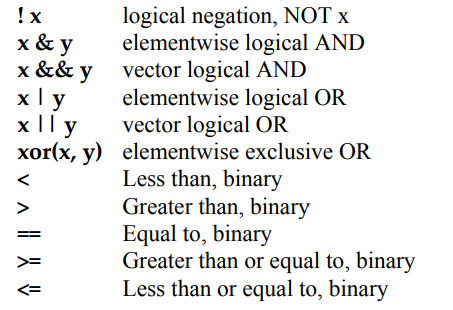
\includegraphics[width=1.5625in,height=\textheight]{images/04/01.PNG}

\begin{Shaded}
\begin{Highlighting}[]
\NormalTok{x }\OtherTok{\textless{}{-}} \DecValTok{2}
\ControlFlowTok{if}\NormalTok{(x}\SpecialCharTok{\%\%}\DecValTok{2} \SpecialCharTok{==} \DecValTok{1}\NormalTok{)\{}
  \FunctionTok{cat}\NormalTok{(}\StringTok{"Odd"}\NormalTok{)}
\NormalTok{\}}\ControlFlowTok{else}\NormalTok{\{}
  \FunctionTok{cat}\NormalTok{(}\StringTok{"Even"}\NormalTok{)}
\NormalTok{\} }

\NormalTok{x }\OtherTok{\textless{}{-}} \DecValTok{5}
\ControlFlowTok{if}\NormalTok{(x }\SpecialCharTok{\textgreater{}} \DecValTok{0} \SpecialCharTok{\&}\NormalTok{ x }\SpecialCharTok{\textless{}} \DecValTok{4}\NormalTok{)\{}
  \FunctionTok{print}\NormalTok{(}\StringTok{"Positive number less than four"}\NormalTok{)}
\NormalTok{\}}

\ControlFlowTok{if}\NormalTok{(x }\SpecialCharTok{\textgreater{}} \DecValTok{0}\NormalTok{) }\FunctionTok{print}\NormalTok{(}\StringTok{"Positive number"}\NormalTok{)}

\NormalTok{x }\OtherTok{\textless{}{-}} \SpecialCharTok{{-}}\DecValTok{5}
\ControlFlowTok{if}\NormalTok{(x }\SpecialCharTok{\textgreater{}} \DecValTok{0}\NormalTok{)\{}
  \FunctionTok{print}\NormalTok{(}\StringTok{"Non{-}negative number"}\NormalTok{)}
\NormalTok{\} }\ControlFlowTok{else} \ControlFlowTok{if}\NormalTok{(x }\SpecialCharTok{\textless{}=} \DecValTok{0} \SpecialCharTok{\&}\NormalTok{ x }\SpecialCharTok{\textgreater{}} \SpecialCharTok{{-}}\DecValTok{5}\NormalTok{)\{}
  \FunctionTok{print}\NormalTok{(}\StringTok{"Negative number greater than {-}5"}\NormalTok{)}
\NormalTok{\} }\ControlFlowTok{else}\NormalTok{ \{}
  \FunctionTok{print}\NormalTok{(}\StringTok{"Negative number less than {-}5"}\NormalTok{)}
\NormalTok{\}}

\ControlFlowTok{if}\NormalTok{(x }\SpecialCharTok{\textgreater{}} \DecValTok{0}\NormalTok{)}
  \FunctionTok{print}\NormalTok{(}\StringTok{"Non{-}negative number"}\NormalTok{)}
\ControlFlowTok{else}
  \FunctionTok{print}\NormalTok{(}\StringTok{"Negative number"}\NormalTok{)}
\end{Highlighting}
\end{Shaded}

\hypertarget{ifelse-statements}{%
\subsection{ifelse statements}\label{ifelse-statements}}

\texttt{if}는 하나의 조건만 비교하는데 사용할 수 있습니다. 그러나 변수에는 여러 값이 벡터형식으로 들어가고 벡터연산을 수행할 경우의 결과도 벡터형식으로 나오지만 \texttt{if}문은 이들을 한 번에 처리하기 어렵습니다. \texttt{ifelse}는 이러한 단점을 보완하여 여러 값을 한번에 처리할 수 있습니다.

\begin{Shaded}
\begin{Highlighting}[]
\FunctionTok{ifelse}\NormalTok{ (condition, True일 때 리턴값, False일 때 리턴값)}
\end{Highlighting}
\end{Shaded}

\texttt{ifelse}의 경우 빠르게 원하는 값을 반환할 수 있으나 조건별로 다른 추가적인 명령의 수행은 불가능하다는 단점이 있습니다.

\begin{Shaded}
\begin{Highlighting}[]

\NormalTok{x }\OtherTok{\textless{}{-}} \FunctionTok{c}\NormalTok{(}\DecValTok{1}\SpecialCharTok{:}\DecValTok{10}\NormalTok{)}
\ControlFlowTok{if}\NormalTok{(x}\SpecialCharTok{\textgreater{}}\DecValTok{10}\NormalTok{)\{}
  \FunctionTok{cat}\NormalTok{(}\StringTok{"Big"}\NormalTok{)}
\NormalTok{\}}\ControlFlowTok{else}\NormalTok{\{}
  \FunctionTok{cat}\NormalTok{(}\StringTok{"Small"}\NormalTok{)}
\NormalTok{\}}

\FunctionTok{ifelse}\NormalTok{(x}\SpecialCharTok{\textgreater{}}\DecValTok{10}\NormalTok{, }\StringTok{"Big"}\NormalTok{, }\StringTok{"Small"}\NormalTok{)}
\end{Highlighting}
\end{Shaded}

\textbf{Exercises}

다음은 median (중간값)을 구하는 공식이며 x의 길이가 (n이) 홀수일 경우와 짝수일 경우에 따라서 다른 공식이 사용된다. 다음 공식과 코드를 이용하여 mymedian 이라는 이름의 함수를 만들고 입력 값들의 중간값을 구해서 반환하는 함수를 만드시오. (\texttt{\%\%} 나머지 연산, \texttt{if}문 사용, 아래 중간값 코드 참고)

\[
median(X) =
\begin{cases}
\frac{1}{2} X[\frac{n}{2}] + \frac{1}{2} X[1+\frac{n}{2}] & \mbox{if } n \mbox{ is even} \\
X[\frac{n+1}{2}] & \mbox{if } n \mbox{ is odd}
\end{cases}
\]

\begin{Shaded}
\begin{Highlighting}[]
\NormalTok{sorted\_x }\OtherTok{\textless{}{-}} \FunctionTok{sort}\NormalTok{(x)}
\CommentTok{\# 만약 짝수이면 }
\NormalTok{retval }\OtherTok{\textless{}{-}}\NormalTok{ sort\_x[n}\SpecialCharTok{/}\DecValTok{2}\NormalTok{]}\SpecialCharTok{/}\DecValTok{2} \SpecialCharTok{+}\NormalTok{ sort\_x[}\DecValTok{1}\SpecialCharTok{+}\NormalTok{(n}\SpecialCharTok{/}\DecValTok{2}\NormalTok{)]}\SpecialCharTok{/}\DecValTok{2}
\CommentTok{\# 만약 홀수이면 }
\NormalTok{retval }\OtherTok{\textless{}{-}}\NormalTok{ sort\_x[(n}\SpecialCharTok{+}\DecValTok{1}\NormalTok{)}\SpecialCharTok{/}\DecValTok{2}\NormalTok{]}
\end{Highlighting}
\end{Shaded}

\hypertarget{for-while-repeat}{%
\subsection{for, while, repeat}\label{for-while-repeat}}

\texttt{for} 문은 반복적으로 특정 코드를 실행하고자 할 때 사용됩니다. 다음과 같은 형식으로 사용할 수 있습니다.

\begin{Shaded}
\begin{Highlighting}[]
\ControlFlowTok{for}\NormalTok{(var }\ControlFlowTok{in}\NormalTok{ seq)\{}
\NormalTok{  expression}
\NormalTok{\}}
\end{Highlighting}
\end{Shaded}

\texttt{var}는 반복을 돌 때마다 바뀌는 변수로 \texttt{\{\}} 안에서 사용되는 지역 변수 입니다. \texttt{seq}는 vector 형식의 변수로 반복을 돌 때마다 순차적으로 \texttt{var}에 저장되는 값들 입니다.

\begin{Shaded}
\begin{Highlighting}[]
\NormalTok{x }\OtherTok{\textless{}{-}} \DecValTok{1}\SpecialCharTok{:}\DecValTok{10}
\ControlFlowTok{for}\NormalTok{(i }\ControlFlowTok{in}\NormalTok{ x)\{}
  \FunctionTok{cat}\NormalTok{(i, }\StringTok{"}\SpecialCharTok{\textbackslash{}n}\StringTok{"}\NormalTok{)}
  \FunctionTok{flush.console}\NormalTok{()}
\NormalTok{\}}

\NormalTok{sum\_of\_i }\OtherTok{\textless{}{-}} \DecValTok{0}
\ControlFlowTok{for}\NormalTok{(i }\ControlFlowTok{in} \DecValTok{1}\SpecialCharTok{:}\DecValTok{10}\NormalTok{)\{}
\NormalTok{  sum\_of\_i }\OtherTok{\textless{}{-}}\NormalTok{ sum\_of\_i }\SpecialCharTok{+}\NormalTok{ i}
  \FunctionTok{cat}\NormalTok{(i, }\StringTok{" "}\NormalTok{, sum\_of\_i, }\StringTok{"}\SpecialCharTok{\textbackslash{}n}\StringTok{"}\NormalTok{);}\FunctionTok{flush.console}\NormalTok{()}
\NormalTok{\}}
\end{Highlighting}
\end{Shaded}

\texttt{while}문도 \texttt{for}문과 같이 반복적으로 특정 코드를 수행하고자 할 때 사용합니다. 사용하는 문법은 다음과 같으며 \texttt{cond}는 \texttt{True} 또는 \texttt{False} 로 반환되는 조건문을 넣고 \texttt{True} 일 경우 계속해서 반복하면서 \texttt{expressions}를 수행하며 이 반복은 \texttt{cond}가 \texttt{False}로 될 때 까지 계속됩니다.

\begin{Shaded}
\begin{Highlighting}[]
\ControlFlowTok{while}\NormalTok{(cond)\{}
\NormalTok{  expression}
\NormalTok{\}}
\end{Highlighting}
\end{Shaded}

\texttt{while}문을 사용할 경우 다음과 같이 \texttt{indicator}라 불리우는 변수를 하나 정해서 반복 할 때마다 값이 바뀌도록 해 주어야 합니다. 그렇지 않으면 무한 루프를 돌게 되는 문제가 발생합니다.

\begin{Shaded}
\begin{Highlighting}[]
\NormalTok{i }\OtherTok{\textless{}{-}} \DecValTok{10}
\NormalTok{f }\OtherTok{\textless{}{-}} \DecValTok{1}
\ControlFlowTok{while}\NormalTok{(i}\SpecialCharTok{\textgreater{}}\DecValTok{1}\NormalTok{)\{}
\NormalTok{  f }\OtherTok{\textless{}{-}}\NormalTok{ i}\SpecialCharTok{*}\NormalTok{f}
\NormalTok{  i }\OtherTok{\textless{}{-}}\NormalTok{ i}\DecValTok{{-}1}
  \FunctionTok{cat}\NormalTok{(i, f, }\StringTok{"}\SpecialCharTok{\textbackslash{}n}\StringTok{"}\NormalTok{)}
\NormalTok{\}}
\NormalTok{f}
\FunctionTok{factorial}\NormalTok{(}\DecValTok{10}\NormalTok{)}
\end{Highlighting}
\end{Shaded}

\texttt{repeat} 명령은 조건 없이 블럭 안에 있는 코드를 무조건 반복하라는 명령 입니다. 따라서 블럭 중간에 멈추기 위한 코드가 필요하고 이 명령이 \texttt{break} 입니다.

\begin{Shaded}
\begin{Highlighting}[]
\ControlFlowTok{repeat}\NormalTok{\{}
\NormalTok{  expressions}
  \ControlFlowTok{if}\NormalTok{(cond) }\ControlFlowTok{break}
\NormalTok{\}}

\NormalTok{i }\OtherTok{\textless{}{-}} \DecValTok{10}
\NormalTok{f }\OtherTok{\textless{}{-}} \DecValTok{1}
\ControlFlowTok{repeat}\NormalTok{ \{}
\NormalTok{  f }\OtherTok{\textless{}{-}}\NormalTok{ i}\SpecialCharTok{*}\NormalTok{f}
\NormalTok{  i }\OtherTok{\textless{}{-}}\NormalTok{ i}\DecValTok{{-}1}
  \FunctionTok{cat}\NormalTok{(i, f, }\StringTok{"}\SpecialCharTok{\textbackslash{}n}\StringTok{"}\NormalTok{)}
  \ControlFlowTok{if}\NormalTok{(i}\SpecialCharTok{\textless{}}\DecValTok{1}\NormalTok{) }\ControlFlowTok{break}
\NormalTok{\}}
\NormalTok{f}
\FunctionTok{factorial}\NormalTok{(}\DecValTok{10}\NormalTok{)}
\end{Highlighting}
\end{Shaded}

\hypertarget{avoiding-loops}{%
\subsection{Avoiding Loops}\label{avoiding-loops}}

R에서는 가능하면 loop문을 사용하지 않는 것이 좋습니다. 이는 다른 언어들 보다 반복문이 느리게 수행된다는 이유 때문이기도 합니다. 그러나 R에서는 반복문을 수행하는 것 보다 훨씬 더 빠르게 반복문을 수행 한 것과 같은 결과를 얻을 수 있는 다양한 방법들이 제공되고 있습니다. 차차 그런 기법들에 대한 학습을 진행하도록 하겠습니다.

\begin{Shaded}
\begin{Highlighting}[]
\NormalTok{x }\OtherTok{\textless{}{-}} \DecValTok{1}\SpecialCharTok{:}\FloatTok{1E7}
\FunctionTok{sum}\NormalTok{(x)}
\FunctionTok{system.time}\NormalTok{(}\FunctionTok{sum}\NormalTok{(x))}

\NormalTok{st }\OtherTok{\textless{}{-}} \FunctionTok{proc.time}\NormalTok{()}
\NormalTok{total }\OtherTok{\textless{}{-}} \DecValTok{0}
\ControlFlowTok{for}\NormalTok{(i }\ControlFlowTok{in} \DecValTok{1}\SpecialCharTok{:}\FunctionTok{length}\NormalTok{(x))\{}
\NormalTok{  total }\OtherTok{\textless{}{-}}\NormalTok{ total }\SpecialCharTok{+}\NormalTok{ x[i]}
\NormalTok{\}}
\NormalTok{ed }\OtherTok{\textless{}{-}} \FunctionTok{proc.time}\NormalTok{()}
\NormalTok{ed}\SpecialCharTok{{-}}\NormalTok{st}
\end{Highlighting}
\end{Shaded}

\textbf{Exercises}

\begin{enumerate}
\def\labelenumi{\arabic{enumi}.}
\tightlist
\item
  다음 네 사람의 이름과 나이를 데이터로 갖는 \texttt{users} 변수를 (data.frame) 만드시오
\end{enumerate}

\begin{Shaded}
\begin{Highlighting}[]
\NormalTok{user\_score }\OtherTok{\textless{}{-}} \FunctionTok{c}\NormalTok{(}\DecValTok{90}\NormalTok{, }\DecValTok{95}\NormalTok{, }\DecValTok{88}\NormalTok{, }\DecValTok{70}\NormalTok{)}
\NormalTok{user\_names }\OtherTok{\textless{}{-}} \FunctionTok{c}\NormalTok{(}\StringTok{"John"}\NormalTok{,}\StringTok{"James"}\NormalTok{,}\StringTok{"Sara"}\NormalTok{, }\StringTok{"Lilly"}\NormalTok{)}
\end{Highlighting}
\end{Shaded}

\begin{enumerate}
\def\labelenumi{\arabic{enumi}.}
\setcounter{enumi}{1}
\tightlist
\item
  각 사람의 점수가 80보다 작으면 \texttt{이름\ 점수:\ Fail} 크면 \texttt{이름\ 점수:\ Pass}를 출력을 하는 코드를 작성하시오. 예를 들어 John의 점수는 80보다 크므로 \texttt{John\ 90:\ Pass} 출력 (\texttt{for}, \texttt{print} 함수 이용)
\end{enumerate}

\hypertarget{object-oriented-programming-advanced}{%
\section{Object Oriented Programming (Advanced)}\label{object-oriented-programming-advanced}}

OOP는 객체지향 프로그래밍 이라고 합니다. OOP를 이용해서 프로그래밍으로 풀고자 하는 문제를 좀 더 명확하게 개념을 수립하고 복잡한 코드를 명료하게 만들 수 있습니다. 그런데 R에서 OOP는 다른 언어보다는 좀 더 어려운 개념적인 이해가 필요합니다. \texttt{S3}, \texttt{S4}, 그리고 \texttt{Reference\ class} 가 있으며 \texttt{S3}, \texttt{S4}는 \texttt{Generic\ function}을 이용하며 다른 언어에서 사용하는 OOP 개념과는 다릅니다. \texttt{Reference\ class}는 다른 언어에서 사용하는 OOP 개념과 유사하며 \texttt{R6} 패키지를 이용해서 사용할 수 있습니다.

\begin{center}\rule{0.5\linewidth}{0.5pt}\end{center}

이 저작물은 크리에이티브 커먼즈 저작자표시-비영리-변경금지 4.0 국제 라이선스에 따라 이용할 수 있습니다.

\hypertarget{data-transformation}{%
\chapter{Data transformation}\label{data-transformation}}

일반적인 데이터 분석은 데이터 전처리(변환), 가시화, 모델링(통계분석)의 반복적인 수행으로 진행될 수 있습니다. R에서는 \texttt{data.frame} 형식의 데이터 타입이 주로 사용되며 (최근 \texttt{tibble}형식) 따라서 \texttt{data.frame} 기반의 데이터를 다루기 위한 다양한 함수를 익힐 필요가 있습니다. 이번 강의에서는 \texttt{data.frame} 데이터를 읽거나 쓰는 함수들과 함께 데이터 전처리를 (변환) 위한 함수들을 배워보겠습니다.

앞에서 배웠던 데이터를 저장하는 object의 종류를 먼저 간략히 정리해 봅니다.

\begin{itemize}
\tightlist
\item
  \textbf{Vectors} - 같은 타입의 데이터를 (Numeric, character, factor, \ldots) 저장한 오브젝트로 인덱스는 \texttt{{[}}, \texttt{{]}} 사용.
\item
  \textbf{Lists} - 여러개의 \texttt{vector}를 원소로 가질 수 있으며 각 원소 vector들은 문자나 숫자 어떤 데이터 타입도 가능하고 길이가 달라도 됨. list의 인덱싱에서 \texttt{{[}} \texttt{{]}}는 리스트를 반환하고 \texttt{{[}{[}} \texttt{{]}{]}}는 vector를 반환함.
\item
  \textbf{Matrices} - 같은 타입의 데이터로 채워진 2차원 행렬이며 인덱스는 \texttt{{[}i,\ j{]}} 형태로 \texttt{i}는 row, \texttt{j}는 column 을 나타냄. 메트릭스의 생성은 \texttt{matrix} 명령어를 사용하며 왼쪽부터 column 값을 모두 채우고 다음 컬럼 값을 채워 나가는 것이 기본 설정임. \texttt{byrow=T} 를 통해 row를 먼저 채울수도 있음. row와 column 이름은 \texttt{rownames}와 \texttt{colnames}로 설정이 가능하며 \texttt{rbind}와 \texttt{cbind}로 두 행렬 또는 행렬과 백터를 연결할 수 있음 ( \texttt{rbind}와 \texttt{cbind}의 경우 행렬이 커지면 컴퓨터 리소스 많이 사용함)
\item
  \textbf{data.frame} - \texttt{list}와 \texttt{matrix}의 특성을 모두 갖는 오브젝트 타입으로 \texttt{list}와 같이 다른 타입의 \texttt{vector}형 변수 여러개가 컬럼에 붙어서 \texttt{matrix} 형태로 구성됨. 단, \texttt{list}와는 다르게 각 변수의 길이가 (row의 길이) 같아야 함. \texttt{\$} 기호로 각 변수들을 인덱싱(접근) 할 수 있고 matrix와 같이 \texttt{{[}i,j{]}} 형태의 인덱싱도 가능.
\end{itemize}

\hypertarget{reading-and-writing}{%
\section{Reading and writing}\label{reading-and-writing}}

파일에 있는 데이터를 R로 읽어들이거나 쓰는 일은 일반적인 데이터 분석 과정에서 필수적일 수 있습니다. 본 강의에서는 일반적으로 사용하는 텍스트 파일과 엑셀파일을 활용하는 방법을 알아보겠습니다.

\hypertarget{text-file}{%
\subsection{Text file}\label{text-file}}

편의상 데이터를 쓰는 과정을 먼저 살펴봅니다. \texttt{UsingR} 예제에 있는 데이터 중 \texttt{batting} 데이터는 2002 야구시즌에 선수들의 정보를 모아둔 데이터 입니다. \texttt{str} 함수로 데이터 전체적인 구조를 파악한 일부 데이터만을 (홈런 개수와 스트라이크 아웃) 이용해 추가적인 데이터를 생성한 후 별도로 파일에 저장해 보겠습니다.

\begin{Shaded}
\begin{Highlighting}[]
\FunctionTok{library}\NormalTok{(UsingR)}
\FunctionTok{data}\NormalTok{(batting)}
\FunctionTok{str}\NormalTok{(batting)}

\NormalTok{mydf }\OtherTok{\textless{}{-}} \FunctionTok{data.frame}\NormalTok{(}\AttributeTok{id =}\NormalTok{ batting}\SpecialCharTok{$}\NormalTok{playerID, }
           \AttributeTok{team =}\NormalTok{ batting}\SpecialCharTok{$}\NormalTok{teamID,}
           \AttributeTok{hr =}\NormalTok{ batting}\SpecialCharTok{$}\NormalTok{HR,}
           \AttributeTok{so =}\NormalTok{ batting}\SpecialCharTok{$}\NormalTok{SO,}
           \AttributeTok{soperhr =}\NormalTok{ batting}\SpecialCharTok{$}\NormalTok{SO}\SpecialCharTok{/}\NormalTok{batting}\SpecialCharTok{$}\NormalTok{HR)}

\FunctionTok{head}\NormalTok{(mydf)}
\end{Highlighting}
\end{Shaded}

재미삼아 홈런과 삼진아웃간의 관계를 한 번 알아보겠습니다.

\begin{Shaded}
\begin{Highlighting}[]
\FunctionTok{plot}\NormalTok{(mydf}\SpecialCharTok{$}\NormalTok{hr, mydf}\SpecialCharTok{$}\NormalTok{so)}
\NormalTok{mycor }\OtherTok{\textless{}{-}} \FunctionTok{cor}\NormalTok{(mydf}\SpecialCharTok{$}\NormalTok{hr, mydf}\SpecialCharTok{$}\NormalTok{so)}
\NormalTok{fit }\OtherTok{\textless{}{-}} \FunctionTok{lm}\NormalTok{(mydf}\SpecialCharTok{$}\NormalTok{so }\SpecialCharTok{\textasciitilde{}}\NormalTok{ mydf}\SpecialCharTok{$}\NormalTok{hr)}
\FunctionTok{plot}\NormalTok{(mydf}\SpecialCharTok{$}\NormalTok{hr, mydf}\SpecialCharTok{$}\NormalTok{so); }\FunctionTok{abline}\NormalTok{(fit); }\FunctionTok{text}\NormalTok{(}\DecValTok{50}\NormalTok{, }\DecValTok{170}\NormalTok{, }\FunctionTok{round}\NormalTok{(mycor,}\DecValTok{2}\NormalTok{))}
\end{Highlighting}
\end{Shaded}

위 데이터를 파일로 저정하기 위해서는 \texttt{write.table} 또는 \texttt{write.csv} 함수를 사용할 수 있습니다. 패키지에 따라서 다양한 함수들이 제공되고 있지만 위 두 파일은 \texttt{utils}라는 R의 기본 패키지에 들어있는 함수들로서 가장 많이 사용되는 함수들 입니다. \texttt{?write.table} 등으로 도움말을 보시고 특히 함수의 전달값 (Arguments) 들을 (\texttt{quote}, \texttt{row.names}, \texttt{col.names}, \texttt{sep}) 익혀두시기 바랍니다.

\begin{Shaded}
\begin{Highlighting}[]

\FunctionTok{write.table}\NormalTok{(mydf, }\AttributeTok{file=}\StringTok{"table\_write.txt"}\NormalTok{)}
\FunctionTok{write.table}\NormalTok{(mydf, }\AttributeTok{file=}\StringTok{"table\_write.txt"}\NormalTok{, }\AttributeTok{quote=}\NormalTok{F)}
\FunctionTok{write.table}\NormalTok{(mydf, }\AttributeTok{file=}\StringTok{"table\_write.txt"}\NormalTok{, }\AttributeTok{quote=}\NormalTok{F, }\AttributeTok{row.names=}\NormalTok{F)}
\FunctionTok{write.table}\NormalTok{(mydf, }\AttributeTok{file=}\StringTok{"table\_write.txt"}\NormalTok{, }\AttributeTok{quote=}\NormalTok{F, }\AttributeTok{row.names=}\NormalTok{F, }\AttributeTok{sep=}\StringTok{","}\NormalTok{)}
\FunctionTok{write.table}\NormalTok{(mydf, }\AttributeTok{file=}\StringTok{"table\_write.csv"}\NormalTok{, }\AttributeTok{quote=}\NormalTok{F, }\AttributeTok{row.names=}\NormalTok{F, }\AttributeTok{sep=}\StringTok{","}\NormalTok{)}
\end{Highlighting}
\end{Shaded}

대부분의 텍스트 파일은 아래와 같이 \texttt{csv} 또는 \texttt{txt} 파일로 저장하여 메모장으로 열어 확인할 수 있으며 읽어올 때 구분자 (sep 파라메터) 나 header를 (header 파라메터) 읽을지 등을 옵션으로 지정할 수 있습니다.

\begin{Shaded}
\begin{Highlighting}[]
\NormalTok{dat }\OtherTok{\textless{}{-}} \FunctionTok{read.csv}\NormalTok{(}\StringTok{"Dataset\_S1\_sub.txt"}\NormalTok{)}
\FunctionTok{head}\NormalTok{(dat)}
\end{Highlighting}
\end{Shaded}

Dataset\_S1\_sub.txt 파일을 열어보면 다음과 같이 header와 ``,''로 구분되어 있는 것을 볼 수 있습니다. \texttt{read.csv} 함수의 도움말을 보면 이 함수의 파라메터 head와 sep이 기본값으로 \texttt{T}와 \texttt{,}로 되어 있는 것을 볼 수 있습니다. \texttt{read.csv} 외에도 \texttt{read.table}, \texttt{read.delim} 등의 함수를 이용해서 택스트 파일을 읽어올 수 있습니다.

\begin{Shaded}
\begin{Highlighting}[]
\FunctionTok{str}\NormalTok{(dat)}
\end{Highlighting}
\end{Shaded}

\textbf{Exercises}

\begin{enumerate}
\def\labelenumi{\arabic{enumi}.}
\tightlist
\item
  위 \texttt{mydf}에서 가장 홈런을 많이 순서로 데이터를 정렬하시오
\item
  위 정렬된 데이터를 \texttt{mydf2} 로 저장한 후 csv 형태의 \texttt{baseball.csv} 파일로 저장하시오
\end{enumerate}

\hypertarget{excel-file}{%
\subsection{Excel file}\label{excel-file}}

텍스트 파일 외에 엑셀파일은 \texttt{readxl} 이라는 R 패키지를 활용하여 읽거나 쓸 수 있습니다. 패키지는 다음과 같은 방법으로 설치할 수 있으며 \texttt{read\_excel} 이라는 함수를 사용해서 데이터를 읽어들일 수 있습니다. 참고로 이 후 강의에서 배우게 될 \texttt{tidyverse} 패키지들 중 \texttt{readr} 패키지를 사용하여 엑셀파일 데이터를 다룰 수도 있습니다.

\begin{Shaded}
\begin{Highlighting}[]
\FunctionTok{install.packages}\NormalTok{(}\StringTok{"readxl"}\NormalTok{)}
\FunctionTok{library}\NormalTok{(readxl)}
\end{Highlighting}
\end{Shaded}

실습 파일은 형광 세포를 배양하여 형광리더기를 이용해 얻어진 실제 데이터이며 \url{plate_reader.xls} 에서 다운로드 받을 수 있습니다. \texttt{read\_excel} 함수를 이용하여 파일의 내용을 읽어오면 기본 자료형이 \texttt{tibble} 입니다. \texttt{tibble}은 최근 많이 쓰이는 R object로 \texttt{data.frame}과 유사하나 입력값의 type, name, rowname을 임으로 바꿀 수 없다는 점이 다릅니다.

\begin{Shaded}
\begin{Highlighting}[]

\NormalTok{dat }\OtherTok{\textless{}{-}} \FunctionTok{read\_excel}\NormalTok{(}\StringTok{"plate\_reader.xls"}\NormalTok{, }\AttributeTok{sheet=}\DecValTok{1}\NormalTok{, }\AttributeTok{skip =} \DecValTok{0}\NormalTok{, }\AttributeTok{col\_names=}\NormalTok{T)}
\end{Highlighting}
\end{Shaded}

엑셀파일에는 두 종류의 (\(OD600_{nm}\), Fluorescence) 데이터가 저장되어 있습니다. 첫 번째 sheet에는 다음처럼 wide형 데이터가 저장되어 있습니다.

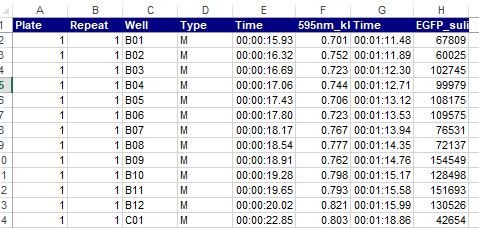
\includegraphics{images/04/excelfile01.PNG}

프로토콜 상세 내역이 나온 세 번째 시트를 읽을 경우 \texttt{sheet} 옵션을 3로 설정하면 되며 skip=3으로 하고 컬럼 이름을 별도로 사용하지 않으므로 \texttt{col\_names=T}로하여 읽을 수 있습니다.

\begin{Shaded}
\begin{Highlighting}[]

\NormalTok{dat }\OtherTok{\textless{}{-}} \FunctionTok{read\_excel}\NormalTok{(}\StringTok{"plate\_reader.xls"}\NormalTok{, }\AttributeTok{sheet=}\DecValTok{3}\NormalTok{, }\AttributeTok{skip =} \DecValTok{3}\NormalTok{, }\AttributeTok{col\_names=}\NormalTok{F)}
\end{Highlighting}
\end{Shaded}

참고로 엑셀파일로 저장하기 위해서는 csv 파일로 데이터를 writing 한 뒤 \texttt{Excel}로 해당 \texttt{csv} 파일을 열고 \texttt{xlsx} 파일로 저장할 수 있습니다.

\hypertarget{subset}{%
\section{Subset}\label{subset}}

R에서 데이터 저장은 \texttt{data.frame}이나 \texttt{matrix} 타입을 일반적으로 사용합니다. 이 데이터의 일부 열 또는 행의 데이터만을 가져와서 별도로 저장하거나 분석이 필요할 경우가 있습니다. 이 때 인덱싱을 사용해서 일부 데이터를 선택하고 사용할 수 있으며 \texttt{subset} 함수도 이러한 선별 기능을 제공합니다. \texttt{subset}은 행과 열 모두를 선별할 수 있는 함수입니다. 다음 \texttt{airquality} 데이터는 1973년 날짜별로 뉴욕의 공기질을 측정한 데이터 입니다. \texttt{NA}를 제외한 나머지 데이터만으로 새로운 데이터셋을 만들어 봅시다. \texttt{is.na}함수를 사용하면 해당 데이터가 \texttt{NA}일 경우 \texttt{TRUE}, \texttt{NA}가 아닐 경우 \texttt{FALSE} 를 반환해 줍니다.

\begin{Shaded}
\begin{Highlighting}[]
\FunctionTok{is.na}\NormalTok{(airquality}\SpecialCharTok{$}\NormalTok{Ozone)}
\NormalTok{ozone\_complete1 }\OtherTok{\textless{}{-}}\NormalTok{ airquality[}\SpecialCharTok{!}\FunctionTok{is.na}\NormalTok{(airquality}\SpecialCharTok{$}\NormalTok{Ozone),]}
\NormalTok{ozone\_complete1 }\OtherTok{\textless{}{-}} \FunctionTok{subset}\NormalTok{(airquality, }\SpecialCharTok{!}\FunctionTok{is.na}\NormalTok{(Ozone))}
\end{Highlighting}
\end{Shaded}

위 ozone\_complete1와 ozone\_complete2는 같은 결과를 보입니다. 그러나 ozone\_complete1 보다는 ozone\_complete2 코드가 훨씬 직관적이고 가독성이 높습니다. 특히 \texttt{airquality\$ozone} 로 \texttt{\$}를 사용하여 변수에 접근한 것이 아닌 \texttt{Ozone}이라는 변수 이름을 직접 사용해서 접근함으로써 코드의 간결성과 가독성을 유지할 수 있습니다. 또한 \texttt{subset}의 \texttt{select} 옵션을 이용해서 변수를 선택할 수도 있으며 \texttt{\&}(AND)와 \texttt{\textbar{}}(OR) 연산자를 사용해서 조건을 두 개 이상 설정할 수 있습니다. 아래 \texttt{select} 옵션에서 \texttt{-}는 해당 변수를 제외한다는 의미 입니다.

\begin{Shaded}
\begin{Highlighting}[]
\NormalTok{ozone\_complete3 }\OtherTok{\textless{}{-}} \FunctionTok{subset}\NormalTok{(airquality, }\SpecialCharTok{!}\FunctionTok{is.na}\NormalTok{(ozone), }\AttributeTok{select=}\FunctionTok{c}\NormalTok{(ozone, temp, month, day))}
\NormalTok{ozone\_complete4 }\OtherTok{\textless{}{-}} \FunctionTok{subset}\NormalTok{(airquality, }\SpecialCharTok{!}\FunctionTok{is.na}\NormalTok{(ozone) }\SpecialCharTok{\&} \SpecialCharTok{!}\FunctionTok{is.na}\NormalTok{(solar.r), }\AttributeTok{select=}\FunctionTok{c}\NormalTok{(}\SpecialCharTok{{-}}\NormalTok{month, }\SpecialCharTok{{-}}\NormalTok{day))}
\end{Highlighting}
\end{Shaded}

\textbf{Exercises}

airquality 데이터에서 \texttt{Temp}와 \texttt{Ozone} 변수로 이루어진 df라는 이름의 \texttt{data.frame}을 만드시오 (단 \texttt{NA}가 있는 샘플(열)은 모두 제외하시오)

\hypertarget{merging-and-split}{%
\section{Merging and Split}\label{merging-and-split}}

\texttt{merge} 함수는 두 개 이상의 데이터셋을 통합하는 기능을 수행하는 함수입니다. 특히 \texttt{rbind}나 \texttt{cbind}와는 다르게, 결합하는 두 데이터에 공통적이거나 한 쪽의 데이터를 기준으로 결합을 수행 합니다. \texttt{?merge}를 참고하면 \texttt{by}, \texttt{by.x}, \texttt{by.y}, \texttt{all}, \texttt{all.x}, \texttt{all.y} 등의 옵션으로 이러한 설정을 수행할 수 있습니다. 간단한 예제를 통해서 이해해 보겠습니다.

10명의 사람이 있고 이 사람들의 나이와 성별을 각각 나타낸 두 데이터셋이 있습니다. 그런데 df1은 나이만을 df2는 성별 정보만을 가지고 있으며 두 정보 모두 제공된 사람은 3명 (인덱스 4,5,6) 뿐입니다. 이제 merge를 이용해서 두 데이터셋을 결합해 보겠습니다.

\begin{Shaded}
\begin{Highlighting}[]
\DocumentationTok{\#\# merge}
\NormalTok{df1 }\OtherTok{\textless{}{-}} \FunctionTok{data.frame}\NormalTok{(}\AttributeTok{id=}\FunctionTok{c}\NormalTok{(}\DecValTok{1}\NormalTok{,}\DecValTok{2}\NormalTok{,}\DecValTok{3}\NormalTok{,}\DecValTok{4}\NormalTok{,}\DecValTok{5}\NormalTok{,}\DecValTok{6}\NormalTok{), }\AttributeTok{age=}\FunctionTok{c}\NormalTok{(}\DecValTok{30}\NormalTok{, }\DecValTok{41}\NormalTok{, }\DecValTok{33}\NormalTok{, }\DecValTok{56}\NormalTok{, }\DecValTok{20}\NormalTok{, }\DecValTok{17}\NormalTok{))}
\NormalTok{df2 }\OtherTok{\textless{}{-}} \FunctionTok{data.frame}\NormalTok{(}\AttributeTok{id=}\FunctionTok{c}\NormalTok{(}\DecValTok{4}\NormalTok{,}\DecValTok{5}\NormalTok{,}\DecValTok{6}\NormalTok{,}\DecValTok{7}\NormalTok{,}\DecValTok{8}\NormalTok{,}\DecValTok{9}\NormalTok{), }\AttributeTok{gender=}\FunctionTok{c}\NormalTok{(}\StringTok{"f"}\NormalTok{, }\StringTok{"f"}\NormalTok{, }\StringTok{"m"}\NormalTok{, }\StringTok{"m"}\NormalTok{, }\StringTok{"f"}\NormalTok{, }\StringTok{"m"}\NormalTok{))}

\NormalTok{df\_inner }\OtherTok{\textless{}{-}} \FunctionTok{merge}\NormalTok{(df1, df2, }\AttributeTok{by=}\StringTok{"id"}\NormalTok{, }\AttributeTok{all=}\NormalTok{F)}
\NormalTok{df\_outer }\OtherTok{\textless{}{-}} \FunctionTok{merge}\NormalTok{(df1, df2, }\AttributeTok{by=}\StringTok{"id"}\NormalTok{, }\AttributeTok{all=}\NormalTok{T)}
\NormalTok{df\_left\_outer }\OtherTok{\textless{}{-}} \FunctionTok{merge}\NormalTok{(df1, df2, }\AttributeTok{by=}\StringTok{"id"}\NormalTok{, }\AttributeTok{all.x=}\NormalTok{T)}
\NormalTok{df\_right\_outer }\OtherTok{\textless{}{-}} \FunctionTok{merge}\NormalTok{(df1, df2, }\AttributeTok{by=}\StringTok{"id"}\NormalTok{, }\AttributeTok{all.y=}\NormalTok{T)}
\end{Highlighting}
\end{Shaded}

만약 두 데이터셋의 id가 다를 경우나 각각 다른 기준으로 결합해야 하는 경우는 \texttt{by}대신 \texttt{by.x}, \texttt{by.y} 옵션을 사용할 수 있습니다.

\texttt{split} 함수는 데이터를 특정 기준으로 나누는 역할을 하며 해당 기준은 factor 형 벡터 형태로 주어질 수 있습니다. 예를 들어 \texttt{airquality} 데이터의 \texttt{month} 변수를 기준으로 데이터를 분리해 보겠습니다.

\begin{Shaded}
\begin{Highlighting}[]
\FunctionTok{str}\NormalTok{(airquality)}
\NormalTok{g }\OtherTok{\textless{}{-}} \FunctionTok{factor}\NormalTok{(airquality}\SpecialCharTok{$}\NormalTok{Month)}
\NormalTok{airq\_split }\OtherTok{\textless{}{-}} \FunctionTok{split}\NormalTok{(airquality, g)}
\FunctionTok{class}\NormalTok{(airq\_split)}
\FunctionTok{str}\NormalTok{(airq\_split)}
\end{Highlighting}
\end{Shaded}

위와 같이 \texttt{airq\_split}은 길이가 5인 (5, 6, 7, 8, 9월) \texttt{list}타입이 되었고 각 요소는 서로 다른 size의 \texttt{data.frame}형으로 구성 된 것을 확인할 수 있습니다.

\hypertarget{transformation}{%
\section{Transformation}\label{transformation}}

R에서 기존 가지고 있는 데이터의 변경은 새로운 변수의 추가, 삭제, 변형과 샘플의 추가, 삭제, 변형을 생각해 볼 수 있습니다. 이러한 기능은 앞에서 배운 \texttt{merge}, \texttt{split}이나 \texttt{rbind}, \texttt{cbind}, 그리고 인덱싱을 활용한 값 변경 등의 방법을 이용할 수 있습니다. 또한 가장 직관적으로 필요한 변수들을 기존 데이터셋에서 추출한 후 \texttt{data.frame} 명령어를 사용해서 새로운 데이터셋으로 만들어주면 될 것 입니다.

이러한 방법들 외에 \texttt{within}을 사용할 경우 특정 변수의 변형과 이를 반영한 새로운 데이터셋을 어렵지 않게 만들수 있습니다. \texttt{with} 함수의 사용 예와 함께 \texttt{within} 함수를 사용하여 데이터를 변형하는 예를 살펴봅니다. \texttt{with}나 \texttt{within} 함수는 R을 활용하는데 많이 사용되는 함수들은 아닙니다. 또한 이러한 기능들은 \texttt{dplyr} 등의 패키지에서 제공하는 경우가 많아서 필수적으로 익힐 부분은 아닙니다. 그러나 개념적인 이해를 돕기위한 좋은 도구들이며 여전히 고수준의 R 사용자들이 코드에 사용하고 있는 함수들이므로 알아두는 것이 좋습니다.

\begin{Shaded}
\begin{Highlighting}[]
\DocumentationTok{\#\# without with}
\NormalTok{ozone\_complete }\OtherTok{\textless{}{-}}\NormalTok{ airquality[}\SpecialCharTok{!}\FunctionTok{is.na}\NormalTok{(airquality}\SpecialCharTok{$}\NormalTok{Ozone),}\StringTok{"Ozone"}\NormalTok{]}
\NormalTok{temp\_complete }\OtherTok{\textless{}{-}}\NormalTok{ airquality[}\SpecialCharTok{!}\FunctionTok{is.na}\NormalTok{(airquality}\SpecialCharTok{$}\NormalTok{Temp),}\StringTok{"Temp"}\NormalTok{]}
\FunctionTok{print}\NormalTok{(}\FunctionTok{mean}\NormalTok{(ozone\_complete))}
\FunctionTok{print}\NormalTok{(}\FunctionTok{mean}\NormalTok{(temp\_complete))}

\DocumentationTok{\#\# with}
\FunctionTok{with}\NormalTok{(airquality, \{}
  \FunctionTok{print}\NormalTok{(}\FunctionTok{mean}\NormalTok{(Ozone[}\SpecialCharTok{!}\FunctionTok{is.na}\NormalTok{(Ozone)]))}
  \FunctionTok{print}\NormalTok{(}\FunctionTok{mean}\NormalTok{(Temp[}\SpecialCharTok{!}\FunctionTok{is.na}\NormalTok{(Temp)]))}
\NormalTok{\})}
\end{Highlighting}
\end{Shaded}

위 \texttt{with} 함수에서 보는바와 같이 \texttt{\$}를 이용한 변수 접근 대신 \texttt{with}함수 내에서는 (\texttt{\{}, \texttt{\}} 안에서) 해당 \texttt{data.frame}에 있는 변수 이름을 직접 접근할 수 있으며 따라서 코드의 간결함과 가독성이 향상됩니다.

\texttt{within} 함수는 \texttt{with}함수와 같이 \texttt{\{}, \texttt{\}} 안에서 변수의 이름만으로 해당 변수에 접근이 가능하나 입력된 데이터와 변경된 변수(들)을 반환한다는 점이 다릅니다. 아래 예는 \texttt{airquality} 데이터의 화씨 (Fahrenheit) 온도를 섭씨 (Celsius) 온도로 변환해서 새로운 데이터셋을 만드는 코드입니다. \texttt{data.frame}을 이용한 코드와 비교해 보시기 바랍니다. 데이터셋 내에서 참조할 변수들이 많아질 경우 \texttt{airquality\$xxx} 식의 코드를 줄이는 것 만으로도 코드의 가독성과 간결성을 유지할 수 있습니다.

\begin{Shaded}
\begin{Highlighting}[]
\NormalTok{newairquality }\OtherTok{\textless{}{-}} \FunctionTok{within}\NormalTok{(airquality, \{}
\NormalTok{  celsius }\OtherTok{=} \FunctionTok{round}\NormalTok{((}\DecValTok{5}\SpecialCharTok{*}\NormalTok{(Temp}\DecValTok{{-}32}\NormalTok{))}\SpecialCharTok{/}\DecValTok{9}\NormalTok{, }\DecValTok{2}\NormalTok{)}
\NormalTok{\})}
\FunctionTok{head}\NormalTok{(newairquality)}

\DocumentationTok{\#\# data.frame}
\NormalTok{celsius }\OtherTok{\textless{}{-}} \FunctionTok{round}\NormalTok{((}\DecValTok{5}\SpecialCharTok{*}\NormalTok{(airquality}\SpecialCharTok{$}\NormalTok{Temp}\DecValTok{{-}32}\NormalTok{))}\SpecialCharTok{/}\DecValTok{9}\NormalTok{, }\DecValTok{2}\NormalTok{)}
\NormalTok{newairquality }\OtherTok{\textless{}{-}} \FunctionTok{data.frame}\NormalTok{(airquality, celsius)}
\FunctionTok{head}\NormalTok{(newairquality)}
\end{Highlighting}
\end{Shaded}

\textbf{Exercises}

다음 df 의 hour, minute, second로 나누어진 값들을 초 단위로 변환하여 seconds라는 변수에 저장한 후 기존 df에 추가한 df2 데이터셋을 만드시오 (\texttt{within} 함수 이용)

\begin{Shaded}
\begin{Highlighting}[]
\NormalTok{df }\OtherTok{\textless{}{-}} \FunctionTok{data.frame}\NormalTok{(}\AttributeTok{hour=}\FunctionTok{c}\NormalTok{(}\DecValTok{4}\NormalTok{, }\DecValTok{7}\NormalTok{, }\DecValTok{1}\NormalTok{, }\DecValTok{5}\NormalTok{, }\DecValTok{8}\NormalTok{),}
                 \AttributeTok{minute=}\FunctionTok{c}\NormalTok{(}\DecValTok{46}\NormalTok{, }\DecValTok{56}\NormalTok{, }\DecValTok{44}\NormalTok{, }\DecValTok{37}\NormalTok{, }\DecValTok{39}\NormalTok{),}
                 \AttributeTok{second=}\FunctionTok{c}\NormalTok{(}\DecValTok{19}\NormalTok{, }\DecValTok{45}\NormalTok{, }\DecValTok{57}\NormalTok{, }\DecValTok{41}\NormalTok{, }\DecValTok{27}\NormalTok{))}
\end{Highlighting}
\end{Shaded}

\hypertarget{babies-example}{%
\section{Babies example}\label{babies-example}}

\texttt{UsingR} 패키지의 \texttt{babies} 데이터를 이용해서 산모의 흡연 여부와 신생아 몸무게의 관계를 알아보는 분석을 수행해 보겠습니다. 본 강의를 통해 배우지 않은 내용들이 있지만 코드를 따라 가면서 참고하시기 바랍니다. 우선 \texttt{UsingR} 패키지를 로딩합니다. 산모의 임신 기간이 (gestation) 999로 표기된 데이터는 명백히 에러이며 이들을 \texttt{NA}로 처리합니다.

\begin{Shaded}
\begin{Highlighting}[]
\FunctionTok{library}\NormalTok{(UsingR)}
\FunctionTok{head}\NormalTok{(babies)}
\DocumentationTok{\#\# a simple way to checkout the data}
\FunctionTok{plot}\NormalTok{(babies}\SpecialCharTok{$}\NormalTok{gestation)  }
\NormalTok{babies}\SpecialCharTok{$}\NormalTok{gestation[babies}\SpecialCharTok{$}\NormalTok{gestation}\SpecialCharTok{\textgreater{}}\DecValTok{900}\NormalTok{] }\OtherTok{\textless{}{-}} \ConstantTok{NA}
\FunctionTok{str}\NormalTok{(babies)}
\end{Highlighting}
\end{Shaded}

아래와 같이 \texttt{within} 함수를 사용해서 \texttt{babies\$} 를 반복해서 입력해주는 불편함을 줄이고 가독성을 높입니다. 똑같은 방법으로 \texttt{dwt} (아빠의 몸무게) 변수의 에러값들에 대해서도 \texttt{NA} 처리를 할 수 있습니다.

\begin{Shaded}
\begin{Highlighting}[]
\NormalTok{new\_babies }\OtherTok{\textless{}{-}} \FunctionTok{within}\NormalTok{(babies, \{}
\NormalTok{  gestation[gestation}\SpecialCharTok{==}\DecValTok{999}\NormalTok{] }\OtherTok{\textless{}{-}} \ConstantTok{NA}
\NormalTok{  dwt[dwt}\SpecialCharTok{==}\DecValTok{999}\NormalTok{] }\OtherTok{\textless{}{-}} \ConstantTok{NA}
\NormalTok{\})}
\FunctionTok{str}\NormalTok{(new\_babies)}
\end{Highlighting}
\end{Shaded}

\texttt{smoke} 변수는 흡연 여부를 나타내는 범주형 변수로 0, 1, 2, 3 값은 의미가 없습니다. 사람이 읽을 수 있는 label을 붙인 \texttt{factor} 형 변수로 변환하는 코드도 함께 작성해 보겠습니다.

\begin{Shaded}
\begin{Highlighting}[]
\FunctionTok{str}\NormalTok{(babies}\SpecialCharTok{$}\NormalTok{smoke)}
\NormalTok{new\_babies }\OtherTok{\textless{}{-}} \FunctionTok{within}\NormalTok{(babies, \{}
\NormalTok{  gestation[gestation}\SpecialCharTok{==}\DecValTok{999}\NormalTok{] }\OtherTok{\textless{}{-}} \ConstantTok{NA}
\NormalTok{  dwt[dwt}\SpecialCharTok{==}\DecValTok{999}\NormalTok{] }\OtherTok{\textless{}{-}} \ConstantTok{NA}
\NormalTok{  smoke }\OtherTok{=} \FunctionTok{factor}\NormalTok{(smoke)}
  \FunctionTok{levels}\NormalTok{(smoke) }\OtherTok{=} \FunctionTok{list}\NormalTok{(}
    \StringTok{"never"} \OtherTok{=} \DecValTok{0}\NormalTok{, }
    \StringTok{"smoke now"} \OtherTok{=} \DecValTok{1}\NormalTok{, }
    \StringTok{"until current pregnancy"} \OtherTok{=} \DecValTok{2}\NormalTok{,}
    \StringTok{"once did, not now"} \OtherTok{=} \DecValTok{3}\NormalTok{)}
\NormalTok{  \})}
\FunctionTok{str}\NormalTok{(new\_babies}\SpecialCharTok{$}\NormalTok{smoke)}
\end{Highlighting}
\end{Shaded}

이제 임신기간과 흡연 여부를 분석해 볼 수 있습니다. 흡연 그룹별로 기간에 차이가 있는지를 알아보는 분석은 \texttt{t-test}나 \texttt{ANOVA}를 사용할 수 있습니다.

\begin{Shaded}
\begin{Highlighting}[]
\NormalTok{fit }\OtherTok{\textless{}{-}} \FunctionTok{lm}\NormalTok{(gestation}\SpecialCharTok{\textasciitilde{}}\NormalTok{smoke, new\_babies)}
\FunctionTok{summary}\NormalTok{(fit) }\DocumentationTok{\#\# t{-}test 결과 }
\FunctionTok{anova}\NormalTok{(fit)}
\end{Highlighting}
\end{Shaded}

간단히 결과를 보면 \texttt{summary(fit)}은 3가지 t-test의 결과를 보여줍니다. never vs.~smoke new 의 경우 t값이 -1.657로 피우지 않은 경우에 비해서 피우는 사람의 임신 기간이 유의하게 줄어들었음을 알 수 있습니다. 그에 비해서 현재 흡연하지 않는 경우 (never vs.~until current pregnancy 또는 never vs.~once did, not now) 차이가 없는 것으로 나옵니다.

이제 smoke now 인 경우 또는 나이가 25세 미만인 경우의 샘플에 대해서 \texttt{newdf}를 만들어 봅니다 (\texttt{subset} 함수 사용, id, gestation, age, wt, smoke 변수 선택). 이 후 \texttt{ggplot}을 이용하여 몸무게와 임신기간의 산점도를 그려보면 크게 다르진 않으나 흡연하는 여성 중 몸무게가 적게 나가는 여성에게서 짧은 임신기간을 갖는 경향을 볼 수 있습니다.

\begin{Shaded}
\begin{Highlighting}[]

\NormalTok{newdf }\OtherTok{\textless{}{-}} \FunctionTok{subset}\NormalTok{(new\_babies, (smoke}\SpecialCharTok{==}\StringTok{"smoke now"} \SpecialCharTok{|}\NormalTok{ smoke }\SpecialCharTok{==} \StringTok{"never"}\NormalTok{) }\SpecialCharTok{\&}\NormalTok{ age }\SpecialCharTok{\textless{}} \DecValTok{25}\NormalTok{, }\AttributeTok{select=}\FunctionTok{c}\NormalTok{(id, gestation, age, wt, smoke))}
\CommentTok{\# ggplot(newdf, aes(x=wt, y=gestation, color=smoke)) +}
\CommentTok{\#   geom\_point(size=3, alpha=0.5) +}
\CommentTok{\#   facet\_grid(.\textasciitilde{}smoke) + }
\CommentTok{\#   theme\_bw()}
\end{Highlighting}
\end{Shaded}

\hypertarget{useful-functions-1}{%
\section{Useful functions}\label{useful-functions-1}}

지금까지 배운 여러 R 프로그래밍 기법이나 함수들과 같이 R을 활용한 데이터 분석에서 자주쓰이거나 유용하게 사용되는 함수들을 소개합니다. 먼저 원소들을 비교하여 공통적 또는 유일한 원소들만을 추출해내는 함수들 입니다.

\begin{Shaded}
\begin{Highlighting}[]
\CommentTok{\#match(), \%in\%, intersect()}

\NormalTok{x }\OtherTok{\textless{}{-}} \DecValTok{1}\SpecialCharTok{:}\DecValTok{10}
\NormalTok{y }\OtherTok{\textless{}{-}} \DecValTok{5}\SpecialCharTok{:}\DecValTok{15}
\FunctionTok{match}\NormalTok{(x, y)}
\NormalTok{x }\SpecialCharTok{\%in\%}\NormalTok{ y}
\FunctionTok{intersect}\NormalTok{(x, y)}

\CommentTok{\#unique()}
\FunctionTok{unique}\NormalTok{(}\FunctionTok{c}\NormalTok{(x, y))}
\end{Highlighting}
\end{Shaded}

다음은 스트링 관련 함수들로서 서열데이터 분석 등에서 유용하게 활용되는 함수들 입니다.

\begin{Shaded}
\begin{Highlighting}[]
\CommentTok{\#substr()}
\NormalTok{x }\OtherTok{\textless{}{-}} \StringTok{"Factors, raw vectors, and lists, are converted"}
\FunctionTok{substr}\NormalTok{(x, }\DecValTok{1}\NormalTok{, }\DecValTok{6}\NormalTok{)}

\CommentTok{\#grep()}
\FunctionTok{grep}\NormalTok{(}\StringTok{"raw"}\NormalTok{, x)}

\CommentTok{\#grepl()}
\FunctionTok{grepl}\NormalTok{(}\StringTok{"raw"}\NormalTok{, x)}
\ControlFlowTok{if}\NormalTok{(}\FunctionTok{grepl}\NormalTok{(}\StringTok{"raw"}\NormalTok{, x))\{}
  \FunctionTok{cat}\NormalTok{(}\StringTok{"I found raw!"}\NormalTok{)}
\NormalTok{\}}

\NormalTok{x }\OtherTok{\textless{}{-}} \FunctionTok{paste}\NormalTok{(LETTERS, }\DecValTok{1}\SpecialCharTok{:}\DecValTok{100}\NormalTok{, }\AttributeTok{sep=}\StringTok{""}\NormalTok{)}
\FunctionTok{grep}\NormalTok{(}\StringTok{"A"}\NormalTok{, x)}
\NormalTok{x[}\FunctionTok{grep}\NormalTok{(}\StringTok{"A"}\NormalTok{, x)]}

\FunctionTok{grepl}\NormalTok{(}\StringTok{"A"}\NormalTok{, x)}
\NormalTok{r }\OtherTok{\textless{}{-}} \FunctionTok{grepl}\NormalTok{(}\StringTok{"A"}\NormalTok{, x)}
\ControlFlowTok{if}\NormalTok{(r)\{}
  \FunctionTok{cat}\NormalTok{(}\StringTok{"Yes, I found A"}\NormalTok{)}
\NormalTok{\}}\ControlFlowTok{else}\NormalTok{\{}
  \FunctionTok{cat}\NormalTok{(}\StringTok{"No A"}\NormalTok{)}
\NormalTok{\}}

\CommentTok{\#strsplit()}
\NormalTok{x }\OtherTok{\textless{}{-}} \FunctionTok{c}\NormalTok{(}\StringTok{"Factors, raw vectors, and lists, are converted"}\NormalTok{, }\StringTok{"vectors, or for, strings with"}\NormalTok{)}
\NormalTok{y }\OtherTok{\textless{}{-}} \FunctionTok{strsplit}\NormalTok{(x, }\AttributeTok{split=}\StringTok{", "}\NormalTok{)}

\CommentTok{\#unlist()}
\FunctionTok{unlist}\NormalTok{(y)}

\NormalTok{y }\OtherTok{\textless{}{-}} \FunctionTok{strsplit}\NormalTok{(x, }\AttributeTok{split=}\StringTok{""}\NormalTok{)}
\NormalTok{ychar }\OtherTok{\textless{}{-}} \FunctionTok{unlist}\NormalTok{(y)}
\NormalTok{ycount }\OtherTok{\textless{}{-}} \FunctionTok{table}\NormalTok{(y2)}
\NormalTok{ycount\_sort }\OtherTok{\textless{}{-}} \FunctionTok{sort}\NormalTok{(ycount)}
\NormalTok{ycount\_sort }\OtherTok{\textless{}{-}} \FunctionTok{sort}\NormalTok{(ycount, }\AttributeTok{decreasing =}\NormalTok{ T)}
\NormalTok{ycount\_top }\OtherTok{\textless{}{-}}\NormalTok{ ycount\_sort[}\DecValTok{1}\SpecialCharTok{:}\DecValTok{5}\NormalTok{]}
\NormalTok{ycount\_top\_char }\OtherTok{\textless{}{-}} \FunctionTok{names}\NormalTok{(ycount\_top)}

\CommentTok{\#toupper(), tolower()}
\FunctionTok{toupper}\NormalTok{(ycount\_top\_char)}
\end{Highlighting}
\end{Shaded}

\textbf{Exercises}

built-in 데이터셋 중 \texttt{state.abb} 은 미국의 50개 주에대한 축약어임.

\begin{enumerate}
\def\labelenumi{\arabic{enumi})}
\item
  이 중 문자 A 가 들어가는 주를 뽑아 x에 저장 하시오 (\texttt{grep} 또는 \texttt{grepl} 사용)
\item
  state.abb 중 위 x에 저장된 이름들을 빼고 y에 저장 하시오 (\texttt{match()} 또는 \texttt{\%in\%}사용)
\item
  state.abb에 사용된 알파벳의 갯수를 구하고 가장 많이 쓰인 알파벳을 구하시오 (\texttt{strsplit()}, \texttt{table()} 등 사용)
\end{enumerate}

\hypertarget{apply}{%
\section{apply}\label{apply}}

\texttt{apply}는 데이터를 변형하기 위한 함수라기 보다는 데이터를 다룰 때 각 원소별, 그룹별, row, 또는 column 별로 반복적으로 수행되는 작업을 효율적으로 수행할 수 있도록 해주는 함수입니다. \texttt{apply} 계열의 함수를 적절히 사용하면 효율성이나 편리성 뿐만 아니라 코드의 간결성 등 많은 장점이 있습니다. 쉬운 이해를 위해 \texttt{colMean} 함수를 예로 들면 \texttt{colMean}은 column 또는 row 단위로 해당하는 모든 값들에 대해 평균을 계산해주는 함수이고 \texttt{apply}를 사용할 경우 다음과 같이 \texttt{apply} 함수와 \texttt{mean} 함수를 이용해서 같은 기능을 수행할 수 있습니다. 아래는 \texttt{babies} 데이터의 clearning 된 (위에서 만들었던) \texttt{new\_babies} 데이터에 이어서 수행되는 내용입니다.

\begin{Shaded}
\begin{Highlighting}[]
\FunctionTok{library}\NormalTok{(UsingR)}
\FunctionTok{head}\NormalTok{(babies)}
\NormalTok{df }\OtherTok{\textless{}{-}} \FunctionTok{subset}\NormalTok{(babies, }\AttributeTok{select=}\FunctionTok{c}\NormalTok{(gestation, wt, dwt))}
\FunctionTok{colMeans}\NormalTok{(df, }\AttributeTok{na.rm=}\NormalTok{T)}
\FunctionTok{apply}\NormalTok{(df, }\DecValTok{2}\NormalTok{, mean, }\AttributeTok{na.rm=}\NormalTok{T)}
\end{Highlighting}
\end{Shaded}

위와 같이 \texttt{colMeans}와 \texttt{apply}가 똑같은 결과를 보여주고 있습니다. 두 번째 인자인 margin의 값으로 (\texttt{?apply}참고) 여기서는 \texttt{2}가 사용되었으며 margin 값이 1인지 2인지에 따라서 다음과 같이 작동을 합니다.

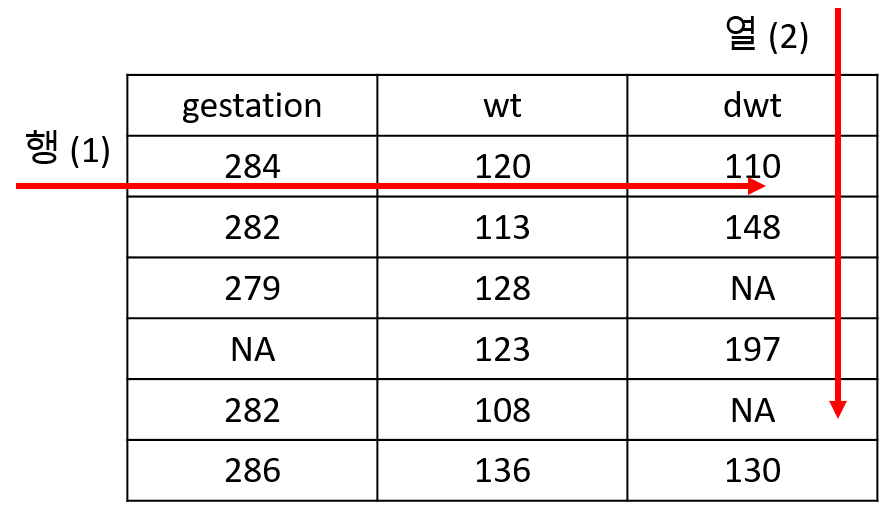
\includegraphics[width=4.16667in,height=\textheight]{images/07/01.png}

\texttt{mean}외에도 다양한 함수들이 사용될 수 있으며 아래와 같이 임의의 함수를 만들어서 사용할 수 도 있습니다. 아래 코드에서는 \texttt{function(x)...}로 바로 함수의 정의를 넣어서 사용했으나 그 아래 \texttt{mysd} 함수와 같이 미리 함수 하나를 만들고 난 후 함수 이름을 이용해서 \texttt{apply}를 적용할 수 있습니다.

\begin{Shaded}
\begin{Highlighting}[]

\FunctionTok{apply}\NormalTok{(df, }\DecValTok{2}\NormalTok{, sd, }\AttributeTok{na.rm=}\NormalTok{T)}
\FunctionTok{apply}\NormalTok{(df, }\DecValTok{2}\NormalTok{, }\ControlFlowTok{function}\NormalTok{(x)\{ }
\NormalTok{  xmean }\OtherTok{\textless{}{-}} \FunctionTok{mean}\NormalTok{(x, }\AttributeTok{na.rm=}\NormalTok{T) }
  \FunctionTok{return}\NormalTok{(xmean)}
\NormalTok{  \})}
\end{Highlighting}
\end{Shaded}

\texttt{apply} 함수는 특히 R에서 느리게 작동하는 loop (\texttt{for}, \texttt{while} 등) 문 대신 사용되어 큰 행렬에 대해서도 빠른 계산 속도를 보여줄 수 있습니다.

\begin{Shaded}
\begin{Highlighting}[]
\NormalTok{n }\OtherTok{\textless{}{-}} \DecValTok{40}
\NormalTok{m }\OtherTok{\textless{}{-}} \FunctionTok{matrix}\NormalTok{(}\FunctionTok{sample}\NormalTok{(}\DecValTok{1}\SpecialCharTok{:}\DecValTok{100}\NormalTok{, n, }\AttributeTok{replace=}\NormalTok{T), }\AttributeTok{ncol=}\DecValTok{4}\NormalTok{)}
\NormalTok{mysd }\OtherTok{\textless{}{-}} \ControlFlowTok{function}\NormalTok{(x)\{}
\NormalTok{  xmean }\OtherTok{\textless{}{-}} \FunctionTok{sum}\NormalTok{(x)}\SpecialCharTok{/}\FunctionTok{length}\NormalTok{(x)}
\NormalTok{  tmpdif }\OtherTok{\textless{}{-}}\NormalTok{ x}\SpecialCharTok{{-}}\NormalTok{xmean}
\NormalTok{  xvar }\OtherTok{\textless{}{-}} \FunctionTok{sum}\NormalTok{(tmpdif}\SpecialCharTok{\^{}}\DecValTok{2}\NormalTok{)}\SpecialCharTok{/}\NormalTok{(}\FunctionTok{length}\NormalTok{(x)}\SpecialCharTok{{-}}\DecValTok{1}\NormalTok{)}
\NormalTok{  xsd }\OtherTok{\textless{}{-}} \FunctionTok{sqrt}\NormalTok{(xvar)}
  \FunctionTok{return}\NormalTok{(xsd)}
\NormalTok{\}}

\DocumentationTok{\#\# for }
\NormalTok{results }\OtherTok{\textless{}{-}} \FunctionTok{rep}\NormalTok{(}\DecValTok{0}\NormalTok{, }\FunctionTok{nrow}\NormalTok{(m))}
\ControlFlowTok{for}\NormalTok{(i }\ControlFlowTok{in} \DecValTok{1}\SpecialCharTok{:}\FunctionTok{nrow}\NormalTok{(m))\{}
\NormalTok{  results[i] }\OtherTok{\textless{}{-}} \FunctionTok{mysd}\NormalTok{(m[i,])}
\NormalTok{\}}
\FunctionTok{print}\NormalTok{(results)}
\FunctionTok{apply}\NormalTok{(m, }\DecValTok{1}\NormalTok{, mysd)}
\FunctionTok{apply}\NormalTok{(m, }\DecValTok{1}\NormalTok{, sd)}
\end{Highlighting}
\end{Shaded}

\texttt{apply} 함수 외에도 \texttt{sapply}, \texttt{lapply}, \texttt{mapply} 등의 다양한 \texttt{apply}계열 함수가 쓰일 수 있습니다. 먼저 \texttt{lapply}는 \texttt{matrix} 형태 데이터가 아닌 \texttt{list} 데이터에 사용되어 각 \texttt{list} 원소별로 주어진 기능을 반복해서 수행하며 \texttt{sapply}는 \texttt{lapply}와 유사하나 벡터, 리스트, 데이터프레임 등에 함수를 적용할 수 있고 그 결과를 벡터 또는 행렬로 반환합니다.

\begin{Shaded}
\begin{Highlighting}[]

\NormalTok{x }\OtherTok{\textless{}{-}} \FunctionTok{list}\NormalTok{(}\AttributeTok{a=}\DecValTok{1}\SpecialCharTok{:}\DecValTok{10}\NormalTok{, }\AttributeTok{b=}\FunctionTok{exp}\NormalTok{(}\SpecialCharTok{{-}}\DecValTok{3}\SpecialCharTok{:}\DecValTok{3}\NormalTok{), }\AttributeTok{logic=}\FunctionTok{c}\NormalTok{(T,T,F,T))}
\FunctionTok{mean}\NormalTok{(x}\SpecialCharTok{$}\NormalTok{a)}
\FunctionTok{lapply}\NormalTok{(x, mean)}
\FunctionTok{sapply}\NormalTok{(x, mean)}

\NormalTok{x }\OtherTok{\textless{}{-}} \FunctionTok{data.frame}\NormalTok{(}\AttributeTok{a=}\DecValTok{1}\SpecialCharTok{:}\DecValTok{10}\NormalTok{, }\AttributeTok{b=}\FunctionTok{exp}\NormalTok{(}\SpecialCharTok{{-}}\DecValTok{4}\SpecialCharTok{:}\DecValTok{5}\NormalTok{))}
\FunctionTok{sapply}\NormalTok{(x, mean)}

\NormalTok{x }\OtherTok{\textless{}{-}} \FunctionTok{c}\NormalTok{(}\DecValTok{4}\NormalTok{, }\DecValTok{9}\NormalTok{, }\DecValTok{16}\NormalTok{)}
\FunctionTok{sapply}\NormalTok{(x, sqrt)}
\FunctionTok{sqrt}\NormalTok{(x)}

\NormalTok{y }\OtherTok{\textless{}{-}} \FunctionTok{c}\NormalTok{(}\DecValTok{1}\SpecialCharTok{:}\DecValTok{10}\NormalTok{)}
\FunctionTok{sapply}\NormalTok{(y, }\ControlFlowTok{function}\NormalTok{(x)\{}\DecValTok{2}\SpecialCharTok{*}\NormalTok{x\})}
\NormalTok{y}\SpecialCharTok{*}\DecValTok{2}
\end{Highlighting}
\end{Shaded}

마지막 예제에서처럼 \texttt{sapply}나 \texttt{lapply}도 임의의 함수를 만들어 적용시킬 수도 있습니다. 자세히 살펴 보면 y는 10개의 값을 갖는 벡터이고 이 벡터의 각 원소 (값에) 함수를 반복해서 적용하는 것 입니다. 함수에서 \texttt{x}는 각 원소의 값을 차례차례 받는 역할을 하므로 1부터 10까지 값이 함수로 들어가 2를 곱한 수가 반환됩니다. 따라서 벡터연산을 하는 \texttt{y*2}와 결과가 같으나 원하는 함수를 정의해서 자유롭게 사용할 수 있다는 장점이 있습니다. 리스트의 경우는 다음과 같이 사용합니다.

\begin{Shaded}
\begin{Highlighting}[]
\NormalTok{y }\OtherTok{\textless{}{-}} \FunctionTok{list}\NormalTok{(}\AttributeTok{a=}\DecValTok{1}\SpecialCharTok{:}\DecValTok{10}\NormalTok{, }\AttributeTok{b=}\FunctionTok{exp}\NormalTok{(}\SpecialCharTok{{-}}\DecValTok{3}\SpecialCharTok{:}\DecValTok{3}\NormalTok{), }\AttributeTok{logic=}\FunctionTok{c}\NormalTok{(T,T,F,T))}
\NormalTok{myfunc }\OtherTok{\textless{}{-}} \ControlFlowTok{function}\NormalTok{(x)\{}
  \FunctionTok{return}\NormalTok{(}\FunctionTok{mean}\NormalTok{(x, }\AttributeTok{na.rm=}\NormalTok{T))}
\NormalTok{\}}
\FunctionTok{lapply}\NormalTok{(y, myfunc)}
\FunctionTok{unlist}\NormalTok{(}\FunctionTok{lapply}\NormalTok{(y, myfunc))}
\end{Highlighting}
\end{Shaded}

즉, \texttt{myfunc}의 \texttt{x}가 list y의 각 원소들, y{[}{[}1{]}{]}, y{[}{[}2{]}{]}, y{[}{[}3{]}{]}를 각각 받아서 \texttt{mean} 연산을 수행해 줍니다. 결과로 각 \texttt{list} 원소들의 평균 값이 반환되며 \texttt{unlist} 함수는 \texttt{list} 형태의 반환 값을 \texttt{vector} 형태로 전환해 줍니다.

\textbf{Exercises}

다음은 앞에서 수행했던 \texttt{airquality} 데이터를 월별로 나눈 데이터셋임. 이 데이터셋을 이용하여 각 월별로 온도와 오존 농도의 평균값을 저장한 \texttt{data.frame} 형식의 데이터를 만들기 위하여 다음 단계별 과정에 적절한 코드를 작성하시오

\begin{Shaded}
\begin{Highlighting}[]
\DocumentationTok{\#\# dataset}
\NormalTok{g }\OtherTok{\textless{}{-}} \FunctionTok{factor}\NormalTok{(airquality}\SpecialCharTok{$}\NormalTok{month)}
\NormalTok{airq\_split }\OtherTok{\textless{}{-}} \FunctionTok{split}\NormalTok{(airquality, g)}
\end{Highlighting}
\end{Shaded}

\begin{enumerate}
\def\labelenumi{\arabic{enumi})}
\tightlist
\item
  다음 \texttt{df}의 \texttt{ozone} 평균을 구하는 \texttt{ozone\_func} 함수를 작성하시오 (단 입력은 \texttt{data.frame} 형식의 오브젝트를 받고 출력은 평균값 (정수 값 하나) 출력. \texttt{mean} 함수 사용시 데이터에 \texttt{NA}가 포함되어 있을 경우 \texttt{na.rm=T} 옵션 적용)
\end{enumerate}

\begin{Shaded}
\begin{Highlighting}[]
\DocumentationTok{\#\# May data.frame}
\NormalTok{df }\OtherTok{\textless{}{-}}\NormalTok{ airq\_split[[}\DecValTok{1}\NormalTok{]]}
\CommentTok{\#}
\CommentTok{\# write your code here for ozone\_func function}
\CommentTok{\#}

\DocumentationTok{\#\# Usage}
\FunctionTok{ozone\_func}\NormalTok{(df)}
\DocumentationTok{\#\# output}
\CommentTok{\# 23.61538}
\end{Highlighting}
\end{Shaded}

\begin{enumerate}
\def\labelenumi{\arabic{enumi})}
\setcounter{enumi}{1}
\item
  \texttt{lapply}와 \texttt{ozone\_func} 함수를 사용하여 \texttt{airq\_split} list 데이터의 월별 \texttt{ozone} 평균 값을 구하고 \texttt{ozone\_means}에 \texttt{vector} 형식으로 저장하시오
\item
  위 1), 2)와 같은 방법으로 \texttt{temp\_func} 함수를 만들고 월별 \texttt{temp}의 평균값을 \texttt{temp\_means}에 \texttt{vector} 형식으로 저장하시오.
\item
  위에서 구해진 두 변수값들을 이용하여 \texttt{air\_means} 라는 이름의 \texttt{data.frame}으로 저장하시오
\end{enumerate}

\begin{center}\rule{0.5\linewidth}{0.5pt}\end{center}

이 저작물은 크리에이티브 커먼즈 저작자표시-비영리-변경금지 4.0 국제 라이선스에 따라 이용할 수 있습니다.

\hypertarget{lecture-note-2}{%
\chapter{Lecture note 2}\label{lecture-note-2}}

설명이나 실습을 위해 \texttt{R\ 사용법\ 및\ 데이터\ 분석\ 기초\ 5.19(목),\ 5.26(목)} 강의를 진행하며 작성한 코드입니다.

\hypertarget{numeric-vector}{%
\section{numeric vector}\label{numeric-vector}}

\begin{itemize}
\tightlist
\item
  Ctrl + Alt + i 누르면 코드청크 생성
\item
  커서를 해당 라인에 두구 Ctrl + Enter 누르면 해당 라인 실행
\end{itemize}

\begin{Shaded}
\begin{Highlighting}[]
\DecValTok{2} \SpecialCharTok{+} \DecValTok{2}
\NormalTok{((}\DecValTok{2{-}1}\NormalTok{)}\SpecialCharTok{\^{}}\DecValTok{2} \SpecialCharTok{+}\NormalTok{ (}\DecValTok{1{-}3}\NormalTok{)}\SpecialCharTok{\^{}}\DecValTok{2}\NormalTok{ )}\SpecialCharTok{\^{}}\NormalTok{(}\DecValTok{1}\SpecialCharTok{/}\DecValTok{2}\NormalTok{)}
\DecValTok{2} \SpecialCharTok{+} \DecValTok{2}\NormalTok{; }\DecValTok{2} \SpecialCharTok{{-}} \DecValTok{2}
\end{Highlighting}
\end{Shaded}

\begin{itemize}
\tightlist
\item
  기억할 단축키

  \begin{itemize}
  \tightlist
  \item
    Ctrl + 1 : 편집창
  \item
    Ctrl + 2 : 콘솔창
  \end{itemize}
\end{itemize}

\begin{Shaded}
\begin{Highlighting}[]
\FunctionTok{sqrt}\NormalTok{((}\DecValTok{4}\SpecialCharTok{+}\DecValTok{3}\NormalTok{)}\SpecialCharTok{*}\NormalTok{(}\DecValTok{2}\SpecialCharTok{+}\DecValTok{1}\NormalTok{))}
\DecValTok{2}\SpecialCharTok{\^{}}\DecValTok{3} \SpecialCharTok{+} \DecValTok{3}\SpecialCharTok{\^{}}\DecValTok{2}
\end{Highlighting}
\end{Shaded}

\begin{itemize}
\tightlist
\item
  변수에 값 저장하기
\end{itemize}

\begin{Shaded}
\begin{Highlighting}[]
\NormalTok{x }\OtherTok{\textless{}{-}} \DecValTok{1}
\NormalTok{y }\OtherTok{\textless{}{-}} \DecValTok{2}
\NormalTok{z }\OtherTok{\textless{}{-}}\NormalTok{ x }\SpecialCharTok{+}\NormalTok{ y}
\end{Highlighting}
\end{Shaded}

\begin{itemize}
\tightlist
\item
  변수 값 보기
\end{itemize}

\begin{Shaded}
\begin{Highlighting}[]
\NormalTok{x}
\NormalTok{y}
\NormalTok{z}
\FunctionTok{print}\NormalTok{(x)}
\FunctionTok{cat}\NormalTok{(x)}
\end{Highlighting}
\end{Shaded}

\begin{itemize}
\tightlist
\item
  numeric vector 만들기
\end{itemize}

\begin{Shaded}
\begin{Highlighting}[]
\NormalTok{x }\OtherTok{\textless{}{-}} \DecValTok{1}\SpecialCharTok{:}\DecValTok{5}
\NormalTok{x}
\NormalTok{y }\OtherTok{\textless{}{-}} \FunctionTok{seq}\NormalTok{(}\DecValTok{1}\NormalTok{, }\DecValTok{5}\NormalTok{, }\DecValTok{1}\NormalTok{)}
\NormalTok{y }\OtherTok{\textless{}{-}} \FunctionTok{seq}\NormalTok{(}\AttributeTok{from=}\DecValTok{1}\NormalTok{, }\AttributeTok{to=}\DecValTok{5}\NormalTok{, }\AttributeTok{by=}\DecValTok{1}\NormalTok{)}
\NormalTok{y }\OtherTok{\textless{}{-}} \FunctionTok{seq}\NormalTok{(}\AttributeTok{to=}\DecValTok{5}\NormalTok{, }\AttributeTok{from=}\DecValTok{1}\NormalTok{, }\AttributeTok{by=}\DecValTok{1}\NormalTok{)}
\NormalTok{y }\OtherTok{\textless{}{-}} \FunctionTok{seq}\NormalTok{(}\DecValTok{5}\NormalTok{, }\DecValTok{1}\NormalTok{, }\SpecialCharTok{{-}}\DecValTok{1}\NormalTok{)}
\NormalTok{?seq}
\NormalTok{y}
\end{Highlighting}
\end{Shaded}

\begin{itemize}
\tightlist
\item
  연습문제 풀이
\end{itemize}

\begin{Shaded}
\begin{Highlighting}[]
\NormalTok{odds }\OtherTok{\textless{}{-}} \FunctionTok{seq}\NormalTok{(}\DecValTok{1}\NormalTok{, }\DecValTok{100}\NormalTok{, }\AttributeTok{by=}\DecValTok{2}\NormalTok{)}
\NormalTok{odds  }
\NormalTok{evens }\OtherTok{\textless{}{-}} \FunctionTok{seq}\NormalTok{(}\DecValTok{2}\NormalTok{, }\DecValTok{100}\NormalTok{, }\DecValTok{2}\NormalTok{)}
\NormalTok{evens}
\end{Highlighting}
\end{Shaded}

\begin{itemize}
\tightlist
\item
  vector의 인덱싱 (첫번째 값의 인덱스는 1부터 시작)
\end{itemize}

\begin{Shaded}
\begin{Highlighting}[]

\NormalTok{odds[}\DecValTok{1}\NormalTok{]}
\NormalTok{odds[}\DecValTok{1}\SpecialCharTok{:}\DecValTok{10}\NormalTok{]}
\NormalTok{i }\OtherTok{\textless{}{-}} \DecValTok{1}\SpecialCharTok{:}\DecValTok{10}
\NormalTok{i}
\NormalTok{odds[i]}
\FunctionTok{dim}\NormalTok{(odds)}
\FunctionTok{length}\NormalTok{(odds)}
\end{Highlighting}
\end{Shaded}

\begin{Shaded}
\begin{Highlighting}[]
\NormalTok{precip}
\NormalTok{?precip}

\FunctionTok{head}\NormalTok{(precip)}
\FunctionTok{str}\NormalTok{(precip)}
\FunctionTok{dim}\NormalTok{(precip)}

\NormalTok{precip[}\DecValTok{1}\NormalTok{]}
\NormalTok{precip[}\StringTok{"Mobile"}\NormalTok{]}
\end{Highlighting}
\end{Shaded}

\begin{itemize}
\tightlist
\item
  logical vector 설명
\item
  기본 그래픽 함수 이용하는 방법은 필요할때만 설명
\end{itemize}

\begin{Shaded}
\begin{Highlighting}[]
\NormalTok{precip}
\FunctionTok{length}\NormalTok{(precip)}
\FunctionTok{plot}\NormalTok{(precip)}
\end{Highlighting}
\end{Shaded}

\begin{itemize}
\tightlist
\item
  \texttt{which} 함수 활용한 40 이상만 선택
\end{itemize}

\begin{Shaded}
\begin{Highlighting}[]
\NormalTok{precip }\SpecialCharTok{\textgreater{}} \DecValTok{40}
\NormalTok{precip[precip }\SpecialCharTok{\textgreater{}} \DecValTok{40}\NormalTok{]}
\NormalTok{idx }\OtherTok{\textless{}{-}}\NormalTok{ precip }\SpecialCharTok{\textgreater{}} \DecValTok{40}
\FunctionTok{which}\NormalTok{(idx)}
\NormalTok{myprecip }\OtherTok{\textless{}{-}}\NormalTok{ precip[}\FunctionTok{which}\NormalTok{(idx)]}
\NormalTok{myprecip}
\FunctionTok{plot}\NormalTok{(myprecip)}
\end{Highlighting}
\end{Shaded}

\begin{itemize}
\tightlist
\item
  \texttt{which}함수 활용한 짝수 만들기
\end{itemize}

\begin{Shaded}
\begin{Highlighting}[]
\NormalTok{mynumers }\OtherTok{\textless{}{-}} \DecValTok{1}\SpecialCharTok{:}\DecValTok{1000}
\NormalTok{mynumers\_res }\OtherTok{\textless{}{-}}\NormalTok{ mynumers }\SpecialCharTok{\%\%} \DecValTok{2}
\NormalTok{i }\OtherTok{\textless{}{-}} \FunctionTok{which}\NormalTok{(mynumers\_res }\SpecialCharTok{==} \DecValTok{0}\NormalTok{)}
\NormalTok{evens }\OtherTok{\textless{}{-}}\NormalTok{ mynumers[i]}
\NormalTok{evens}
\end{Highlighting}
\end{Shaded}

\begin{itemize}
\tightlist
\item
  홀수 값을 저장하는 벡터 만들고 하나씩 샘플링 (\texttt{sample} 함수 사용)
\end{itemize}

\begin{Shaded}
\begin{Highlighting}[]
\NormalTok{odds }\OtherTok{\textless{}{-}} \FunctionTok{seq}\NormalTok{(}\DecValTok{1}\NormalTok{, }\DecValTok{1000}\NormalTok{, }\DecValTok{2}\NormalTok{)}
\FunctionTok{length}\NormalTok{(evens)}
\FunctionTok{length}\NormalTok{(odds)}
\NormalTok{?sample}
\NormalTok{mysample }\OtherTok{\textless{}{-}} \FunctionTok{c}\NormalTok{(}\FunctionTok{sample}\NormalTok{(evens, }\DecValTok{1}\NormalTok{), }\FunctionTok{sample}\NormalTok{(odds, }\DecValTok{1}\NormalTok{))}
\FunctionTok{print}\NormalTok{(mysample[}\DecValTok{1}\NormalTok{])}
\end{Highlighting}
\end{Shaded}

\begin{itemize}
\tightlist
\item
  문자열 붙이기, \texttt{,}로 나누어진 벡터들 각각의 원소를 붙여줌
\end{itemize}

\begin{Shaded}
\begin{Highlighting}[]
\FunctionTok{paste}\NormalTok{(}\StringTok{"X"}\NormalTok{, }\StringTok{"Y"}\NormalTok{, }\StringTok{"Z"}\NormalTok{, }\AttributeTok{sep=}\StringTok{"\_"}\NormalTok{)}
\FunctionTok{paste}\NormalTok{(}\StringTok{"X"}\NormalTok{, }\StringTok{"Y"}\NormalTok{, }\StringTok{"Z"}\NormalTok{, }\AttributeTok{sep=}\StringTok{""}\NormalTok{)}
\FunctionTok{paste}\NormalTok{(}\StringTok{"X"}\NormalTok{, }\StringTok{"Y"}\NormalTok{, }\StringTok{"Z"}\NormalTok{, }\StringTok{"X"}\NormalTok{, }\StringTok{"Y"}\NormalTok{, }\StringTok{"Z"}\NormalTok{, }\StringTok{"X"}\NormalTok{, }\AttributeTok{sep=}\StringTok{""}\NormalTok{)}
\end{Highlighting}
\end{Shaded}

\begin{itemize}
\tightlist
\item
  여러 벡터에서 각각의 원소를 붙여주는 기능
\end{itemize}

\begin{Shaded}
\begin{Highlighting}[]
\FunctionTok{paste}\NormalTok{(}\FunctionTok{c}\NormalTok{(}\StringTok{"X"}\NormalTok{,}\StringTok{"Y"}\NormalTok{), }\DecValTok{1}\SpecialCharTok{:}\DecValTok{10}\NormalTok{, }\AttributeTok{sep=}\StringTok{""}\NormalTok{)}

\NormalTok{gene\_names }\OtherTok{\textless{}{-}} \FunctionTok{paste}\NormalTok{(}\StringTok{"gene"}\NormalTok{, }\DecValTok{1}\SpecialCharTok{:}\DecValTok{100}\NormalTok{, }\AttributeTok{sep=}\StringTok{""}\NormalTok{)}
\end{Highlighting}
\end{Shaded}

\begin{itemize}
\tightlist
\item
  collapse (하나의 벡터에서 해당 벡터의 원소들을 붙여주는 기능)
\end{itemize}

\begin{Shaded}
\begin{Highlighting}[]
\FunctionTok{paste}\NormalTok{(}\FunctionTok{c}\NormalTok{(}\StringTok{"X"}\NormalTok{, }\StringTok{"Y"}\NormalTok{), }\AttributeTok{collapse =} \StringTok{""}\NormalTok{)}
\end{Highlighting}
\end{Shaded}

\begin{itemize}
\tightlist
\item
  예제 (\texttt{sample()}, \texttt{paste()}, \texttt{rep()})
\end{itemize}

\begin{Shaded}
\begin{Highlighting}[]

\NormalTok{x }\OtherTok{\textless{}{-}} \FunctionTok{sample}\NormalTok{(}\FunctionTok{c}\NormalTok{(}\StringTok{"A"}\NormalTok{, }\StringTok{"C"}\NormalTok{, }\StringTok{"G"}\NormalTok{, }\StringTok{"T"}\NormalTok{), }\AttributeTok{size=}\DecValTok{20}\NormalTok{, }\AttributeTok{replace =}\NormalTok{ T)}
\NormalTok{x2 }\OtherTok{\textless{}{-}} \FunctionTok{paste}\NormalTok{(x, }\AttributeTok{collapse =} \StringTok{""}\NormalTok{)}

\NormalTok{myseq }\OtherTok{\textless{}{-}} \FunctionTok{rep}\NormalTok{(}\StringTok{""}\NormalTok{, }\DecValTok{5}\NormalTok{)}
\NormalTok{myseq[}\DecValTok{1}\NormalTok{] }\OtherTok{\textless{}{-}} \FunctionTok{paste}\NormalTok{(}\FunctionTok{sample}\NormalTok{(}\FunctionTok{c}\NormalTok{(}\StringTok{"A"}\NormalTok{, }\StringTok{"C"}\NormalTok{, }\StringTok{"G"}\NormalTok{, }\StringTok{"T"}\NormalTok{), }\AttributeTok{size=}\DecValTok{20}\NormalTok{, }\AttributeTok{replace =}\NormalTok{ T), }\AttributeTok{collapse=}\StringTok{""}\NormalTok{)}
\NormalTok{myseq[}\DecValTok{2}\NormalTok{] }\OtherTok{\textless{}{-}} \FunctionTok{paste}\NormalTok{(}\FunctionTok{sample}\NormalTok{(}\FunctionTok{c}\NormalTok{(}\StringTok{"A"}\NormalTok{, }\StringTok{"C"}\NormalTok{, }\StringTok{"G"}\NormalTok{, }\StringTok{"T"}\NormalTok{), }\AttributeTok{size=}\DecValTok{20}\NormalTok{, }\AttributeTok{replace =}\NormalTok{ T), }\AttributeTok{collapse=}\StringTok{""}\NormalTok{)}
\NormalTok{myseq[}\DecValTok{3}\NormalTok{] }\OtherTok{\textless{}{-}} \FunctionTok{paste}\NormalTok{(}\FunctionTok{sample}\NormalTok{(}\FunctionTok{c}\NormalTok{(}\StringTok{"A"}\NormalTok{, }\StringTok{"C"}\NormalTok{, }\StringTok{"G"}\NormalTok{, }\StringTok{"T"}\NormalTok{), }\AttributeTok{size=}\DecValTok{20}\NormalTok{, }\AttributeTok{replace =}\NormalTok{ T), }\AttributeTok{collapse=}\StringTok{""}\NormalTok{)}
\NormalTok{myseq[}\DecValTok{4}\NormalTok{] }\OtherTok{\textless{}{-}} \FunctionTok{paste}\NormalTok{(}\FunctionTok{sample}\NormalTok{(}\FunctionTok{c}\NormalTok{(}\StringTok{"A"}\NormalTok{, }\StringTok{"C"}\NormalTok{, }\StringTok{"G"}\NormalTok{, }\StringTok{"T"}\NormalTok{), }\AttributeTok{size=}\DecValTok{20}\NormalTok{, }\AttributeTok{replace =}\NormalTok{ T), }\AttributeTok{collapse=}\StringTok{""}\NormalTok{)}
\NormalTok{myseq[}\DecValTok{5}\NormalTok{] }\OtherTok{\textless{}{-}} \FunctionTok{paste}\NormalTok{(}\FunctionTok{sample}\NormalTok{(}\FunctionTok{c}\NormalTok{(}\StringTok{"A"}\NormalTok{, }\StringTok{"C"}\NormalTok{, }\StringTok{"G"}\NormalTok{, }\StringTok{"T"}\NormalTok{), }\AttributeTok{size=}\DecValTok{20}\NormalTok{, }\AttributeTok{replace =}\NormalTok{ T), }\AttributeTok{collapse=}\StringTok{""}\NormalTok{)}

\NormalTok{myseq}
\end{Highlighting}
\end{Shaded}

\begin{itemize}
\tightlist
\item
  예제 `TAAGTCT' 바코드를 각 서열의 3'에 붙여보기
\end{itemize}

\begin{Shaded}
\begin{Highlighting}[]
\FunctionTok{paste}\NormalTok{(myseq, }\FunctionTok{c}\NormalTok{(}\StringTok{"TAAGTCT"}\NormalTok{), }\AttributeTok{sep=}\StringTok{""}\NormalTok{)}
\FunctionTok{strsplit}\NormalTok{(}\StringTok{"XYZ"}\NormalTok{, }\AttributeTok{split=}\StringTok{""}\NormalTok{)}
\end{Highlighting}
\end{Shaded}

\begin{itemize}
\tightlist
\item
  \texttt{split} 함수 사용
\end{itemize}

\begin{Shaded}
\begin{Highlighting}[]
\NormalTok{x }\OtherTok{\textless{}{-}} \FunctionTok{strsplit}\NormalTok{(}\StringTok{"XYZ"}\NormalTok{, }\AttributeTok{split=}\StringTok{""}\NormalTok{)}
\FunctionTok{class}\NormalTok{(x)}
\NormalTok{x}
\NormalTok{y }\OtherTok{\textless{}{-}} \FunctionTok{unlist}\NormalTok{(x)}
\FunctionTok{class}\NormalTok{(y)}
\NormalTok{y}
\end{Highlighting}
\end{Shaded}

\begin{itemize}
\tightlist
\item
  \texttt{factor} 간단한 설명
\end{itemize}

\begin{Shaded}
\begin{Highlighting}[]
\NormalTok{x }\OtherTok{\textless{}{-}} \FunctionTok{c}\NormalTok{(}\StringTok{"Red"}\NormalTok{, }\StringTok{"Blue"}\NormalTok{, }\StringTok{"Yellow"}\NormalTok{, }\StringTok{"Red"}\NormalTok{, }\StringTok{"Blue"}\NormalTok{)}
\NormalTok{x}
\NormalTok{y }\OtherTok{\textless{}{-}} \FunctionTok{factor}\NormalTok{(x)}
\NormalTok{y}
\NormalTok{y[}\DecValTok{1}\NormalTok{] }\OtherTok{\textless{}{-}} \StringTok{"gold"}

\FunctionTok{levels}\NormalTok{(y)[}\DecValTok{4}\NormalTok{] }\OtherTok{\textless{}{-}} \StringTok{"gold"}
\NormalTok{y}
\NormalTok{y[}\DecValTok{1}\NormalTok{] }\OtherTok{\textless{}{-}} \StringTok{"gold"}
\NormalTok{y}
\end{Highlighting}
\end{Shaded}

\begin{itemize}
\tightlist
\item
  데이터에서 \texttt{factor}들 보기
\end{itemize}

\begin{Shaded}
\begin{Highlighting}[]
\FunctionTok{library}\NormalTok{(MASS)}
\NormalTok{Cars93}
\FunctionTok{str}\NormalTok{(Cars93)}
\end{Highlighting}
\end{Shaded}

\begin{itemize}
\tightlist
\item
  아미노산 및 각 아미노산에 해당하는 코돈 표현 예제
\end{itemize}

\begin{Shaded}
\begin{Highlighting}[]

\NormalTok{aa }\OtherTok{\textless{}{-}} \FunctionTok{c}\NormalTok{(}\StringTok{"Phe"}\NormalTok{, }\StringTok{"Leu"}\NormalTok{, }\StringTok{"Ser"}\NormalTok{)}
\FunctionTok{class}\NormalTok{(aa)}
\NormalTok{aa }\OtherTok{\textless{}{-}} \FunctionTok{factor}\NormalTok{(aa)}
\FunctionTok{class}\NormalTok{(aa)}

\NormalTok{aa }\OtherTok{\textless{}{-}} \FunctionTok{list}\NormalTok{()}
\NormalTok{aa[[}\DecValTok{1}\NormalTok{]] }\OtherTok{\textless{}{-}} \FunctionTok{c}\NormalTok{(}\StringTok{"UUU"}\NormalTok{, }\StringTok{"UUC"}\NormalTok{)}
\NormalTok{aa}
\NormalTok{aa[[}\DecValTok{2}\NormalTok{]] }\OtherTok{\textless{}{-}} \FunctionTok{c}\NormalTok{(}\StringTok{"UUA"}\NormalTok{, }\StringTok{"UUG"}\NormalTok{, }\StringTok{"CUA"}\NormalTok{, }\StringTok{"CUU"}\NormalTok{, }\StringTok{"CUG"}\NormalTok{, }\StringTok{"CUC"}\NormalTok{)}
\NormalTok{aa}
\FunctionTok{class}\NormalTok{(aa)}
\FunctionTok{names}\NormalTok{(aa) }\OtherTok{\textless{}{-}} \FunctionTok{c}\NormalTok{(}\StringTok{"Phe"}\NormalTok{, }\StringTok{"Leu"}\NormalTok{)}
\NormalTok{aa}
\NormalTok{aa[[}\DecValTok{1}\NormalTok{]][}\DecValTok{1}\NormalTok{]}
\NormalTok{aa[[}\DecValTok{2}\NormalTok{]][}\DecValTok{3}\NormalTok{]}
\end{Highlighting}
\end{Shaded}

\begin{itemize}
\tightlist
\item
  useful functions
\end{itemize}

\begin{Shaded}
\begin{Highlighting}[]
\NormalTok{z }\OtherTok{\textless{}{-}} \FunctionTok{sample}\NormalTok{(}\DecValTok{1}\SpecialCharTok{:}\DecValTok{10}\NormalTok{, }\DecValTok{100}\NormalTok{, T)}
\NormalTok{?sample}
\NormalTok{z}
\FunctionTok{head}\NormalTok{(z)}
\FunctionTok{sort}\NormalTok{(z)}
\FunctionTok{order}\NormalTok{(z)}
\FunctionTok{table}\NormalTok{(z)}
\end{Highlighting}
\end{Shaded}

\hypertarget{matrix-1}{%
\section{matrix}\label{matrix-1}}

\begin{itemize}
\tightlist
\item
  연습문제 풀이 성적별 테이블 정렬
\end{itemize}

\begin{Shaded}
\begin{Highlighting}[]
\NormalTok{mynum }\OtherTok{\textless{}{-}} \FunctionTok{sample}\NormalTok{(}\DecValTok{1}\SpecialCharTok{:}\DecValTok{100}\NormalTok{, }\DecValTok{20}\NormalTok{, T)}
\NormalTok{mynum}
\NormalTok{score }\OtherTok{\textless{}{-}} \FunctionTok{matrix}\NormalTok{(mynum, }\AttributeTok{nrow =} \DecValTok{10}\NormalTok{, }\AttributeTok{ncol =} \DecValTok{2}\NormalTok{)}
\NormalTok{score}
\NormalTok{myrowname }\OtherTok{\textless{}{-}} \FunctionTok{paste}\NormalTok{(}\StringTok{"Name"}\NormalTok{, }\DecValTok{1}\SpecialCharTok{:}\DecValTok{10}\NormalTok{, }\AttributeTok{sep=}\StringTok{""}\NormalTok{)}
\NormalTok{myrowname}
\FunctionTok{rownames}\NormalTok{(score) }\OtherTok{\textless{}{-}}\NormalTok{ myrowname}
\NormalTok{score}
\FunctionTok{colnames}\NormalTok{(score) }\OtherTok{\textless{}{-}} \FunctionTok{c}\NormalTok{(}\StringTok{"Math"}\NormalTok{, }\StringTok{"Eng"}\NormalTok{)}

\NormalTok{total\_score }\OtherTok{\textless{}{-}}\NormalTok{ score[,}\DecValTok{1}\NormalTok{] }\SpecialCharTok{+}\NormalTok{ score[,}\DecValTok{2}\NormalTok{]}
\NormalTok{total\_score }\OtherTok{\textless{}{-}}\NormalTok{ score[,}\StringTok{"Math"}\NormalTok{] }\SpecialCharTok{+}\NormalTok{ score[,}\StringTok{"Eng"}\NormalTok{]}
\FunctionTok{sort}\NormalTok{(total\_score, }\AttributeTok{decreasing =}\NormalTok{ T)}
\NormalTok{score}
\NormalTok{o }\OtherTok{\textless{}{-}} \FunctionTok{order}\NormalTok{(total\_score, }\AttributeTok{decreasing =}\NormalTok{ T)}
\NormalTok{o}
\NormalTok{score[o,]}
\end{Highlighting}
\end{Shaded}

\hypertarget{data.frame-1}{%
\section{data.frame}\label{data.frame-1}}

\begin{Shaded}
\begin{Highlighting}[]

\NormalTok{math\_score }\OtherTok{\textless{}{-}} \FunctionTok{sample}\NormalTok{(}\DecValTok{1}\SpecialCharTok{:}\DecValTok{100}\NormalTok{, }\DecValTok{10}\NormalTok{, T)}
\NormalTok{eng\_score }\OtherTok{\textless{}{-}} \FunctionTok{sample}\NormalTok{(}\DecValTok{1}\SpecialCharTok{:}\DecValTok{100}\NormalTok{, }\DecValTok{10}\NormalTok{, T)}
\NormalTok{score }\OtherTok{\textless{}{-}} \FunctionTok{data.frame}\NormalTok{(math\_score, eng\_score)}
\NormalTok{score}
\NormalTok{score}\SpecialCharTok{$}\NormalTok{math\_score}
\NormalTok{score}\SpecialCharTok{$}\NormalTok{eng\_score}
\end{Highlighting}
\end{Shaded}

\begin{itemize}
\tightlist
\item
  추가 연습문제: 수학, 영어 성적을 더해서 \texttt{total\_score}를 만들고 이 값을 기준으로 내림차순으로 score 데이터프레임을 정렬 하시오.
\end{itemize}

\begin{Shaded}
\begin{Highlighting}[]
\NormalTok{total\_score }\OtherTok{\textless{}{-}}\NormalTok{ score}\SpecialCharTok{$}\NormalTok{math\_score }\SpecialCharTok{+}\NormalTok{ score}\SpecialCharTok{$}\NormalTok{eng\_score}
\NormalTok{o }\OtherTok{\textless{}{-}} \FunctionTok{order}\NormalTok{(total\_score, }\AttributeTok{decreasing =}\NormalTok{ T)}
\NormalTok{score[o,]}
\end{Highlighting}
\end{Shaded}

\hypertarget{list-1}{%
\section{list}\label{list-1}}

\begin{Shaded}
\begin{Highlighting}[]
\NormalTok{score}
\FunctionTok{class}\NormalTok{(score)}
\NormalTok{mynum}
\FunctionTok{class}\NormalTok{(mynum)}

\NormalTok{z }\OtherTok{\textless{}{-}} \FunctionTok{list}\NormalTok{()}
\NormalTok{z[[}\DecValTok{1}\NormalTok{]] }\OtherTok{\textless{}{-}}\NormalTok{ score}
\NormalTok{z[[}\DecValTok{2}\NormalTok{]] }\OtherTok{\textless{}{-}}\NormalTok{ mynum}
\NormalTok{z}
\FunctionTok{names}\NormalTok{(z) }\OtherTok{\textless{}{-}} \FunctionTok{c}\NormalTok{(}\StringTok{"dataframe"}\NormalTok{, }\StringTok{"numericvector"}\NormalTok{)}
\NormalTok{z}
\NormalTok{z}\SpecialCharTok{$}\NormalTok{dataframe}
\NormalTok{z}\SpecialCharTok{$}\NormalTok{numericvector}
\end{Highlighting}
\end{Shaded}

\begin{itemize}
\tightlist
\item
  리스트 만들때 미리 원소의 개수를 알고 있으면 그 원소의 개수에 맞게 생성해 주는 것이 좋음 \texttt{aa\ \textless{}-\ vector("list",\ 5)}
\item
  각 아미노산에 해당하는 코돈 길이가 달라도 list 형태로 저장 가능
\end{itemize}

\begin{Shaded}
\begin{Highlighting}[]
\NormalTok{aa }\OtherTok{\textless{}{-}} \FunctionTok{list}\NormalTok{()}
\NormalTok{aa[[}\DecValTok{1}\NormalTok{]] }\OtherTok{\textless{}{-}} \FunctionTok{c}\NormalTok{(}\StringTok{"UUU"}\NormalTok{, }\StringTok{"UUC"}\NormalTok{)}
\NormalTok{aa}
\NormalTok{aa[[}\DecValTok{2}\NormalTok{]] }\OtherTok{\textless{}{-}} \FunctionTok{c}\NormalTok{(}\StringTok{"UUA"}\NormalTok{, }\StringTok{"UUG"}\NormalTok{, }\StringTok{"CUA"}\NormalTok{, }\StringTok{"CUU"}\NormalTok{, }\StringTok{"CUG"}\NormalTok{, }\StringTok{"CUC"}\NormalTok{)}
\NormalTok{aa}
\FunctionTok{class}\NormalTok{(aa)}
\FunctionTok{names}\NormalTok{(aa) }\OtherTok{\textless{}{-}} \FunctionTok{c}\NormalTok{(}\StringTok{"Phe"}\NormalTok{, }\StringTok{"Leu"}\NormalTok{)}
\NormalTok{aa}

\FunctionTok{as.data.frame}\NormalTok{(aa)}
\end{Highlighting}
\end{Shaded}

\begin{itemize}
\tightlist
\item
  바람직한 데이터는 column은 변수, row는 샘플 구조의 데이터. 예를 들어서, 변수:먹이, 수명 --\textgreater{} 컬럼, 샘플: 마우스1, 마우스2 --\textgreater{} Row, 등
\end{itemize}

\begin{Shaded}
\begin{Highlighting}[]
\NormalTok{aa }\OtherTok{\textless{}{-}} \FunctionTok{c}\NormalTok{(}\StringTok{"Phe"}\NormalTok{, }\StringTok{"Leu"}\NormalTok{)}
\NormalTok{codon }\OtherTok{\textless{}{-}} \FunctionTok{c}\NormalTok{(}\StringTok{"UUU"}\NormalTok{, }\StringTok{"UUC"}\NormalTok{, }\StringTok{"UUA"}\NormalTok{, }\StringTok{"UUG"}\NormalTok{, }\StringTok{"CUA"}\NormalTok{, }\StringTok{"CUU"}\NormalTok{, }\StringTok{"CUG"}\NormalTok{, }\StringTok{"CUC"}\NormalTok{)}
\FunctionTok{data.frame}\NormalTok{(aa, codon)}
\NormalTok{aa }\OtherTok{\textless{}{-}} \FunctionTok{c}\NormalTok{(}\FunctionTok{rep}\NormalTok{(}\StringTok{"Phe"}\NormalTok{, }\DecValTok{2}\NormalTok{), }\FunctionTok{rep}\NormalTok{(}\StringTok{"Leu"}\NormalTok{,}\DecValTok{6}\NormalTok{))}
\NormalTok{codon }\OtherTok{\textless{}{-}} \FunctionTok{c}\NormalTok{(}\StringTok{"UUU"}\NormalTok{, }\StringTok{"UUC"}\NormalTok{, }\StringTok{"UUA"}\NormalTok{, }\StringTok{"UUG"}\NormalTok{, }\StringTok{"CUA"}\NormalTok{, }\StringTok{"CUU"}\NormalTok{, }\StringTok{"CUG"}\NormalTok{, }\StringTok{"CUC"}\NormalTok{)}
\FunctionTok{data.frame}\NormalTok{(aa, codon)}
\end{Highlighting}
\end{Shaded}

\hypertarget{functions-1}{%
\section{functions}\label{functions-1}}

\begin{Shaded}
\begin{Highlighting}[]
\FunctionTok{source}\NormalTok{(}\StringTok{"myscript.R"}\NormalTok{)}
\end{Highlighting}
\end{Shaded}

\begin{itemize}
\tightlist
\item
  함수만들기
\end{itemize}

\begin{verbatim}
my_function_name <- function(parameter1, parameter2, ... ){
  ##any statements
  return(object)
}
\end{verbatim}

\begin{Shaded}
\begin{Highlighting}[]

\DocumentationTok{\#\# mynumers: numeric vector}
\NormalTok{mymean }\OtherTok{\textless{}{-}} \ControlFlowTok{function}\NormalTok{(mynumers)\{}
  \CommentTok{\#cat("Input numbers are", mynumers, "\textbackslash{}n")}
\NormalTok{  numbers\_mean }\OtherTok{\textless{}{-}} \FunctionTok{sum}\NormalTok{(mynumers)}\SpecialCharTok{/}\FunctionTok{length}\NormalTok{(mynumers)}
  \CommentTok{\#out \textless{}{-} paste("The average is ", numbers\_mean, ".\textbackslash{}n", sep="")}
  \CommentTok{\#cat(out)}
  \FunctionTok{return}\NormalTok{(numbers\_mean)}
\NormalTok{\}}
\end{Highlighting}
\end{Shaded}

\begin{itemize}
\tightlist
\item
  함수 만든 후 loading 할 때 \texttt{\{}, \texttt{\}} 밖에서 Ctrl + Enter로 로딩
\end{itemize}

\begin{Shaded}
\begin{Highlighting}[]
\FunctionTok{mymean}\NormalTok{(}\FunctionTok{c}\NormalTok{(}\DecValTok{1}\NormalTok{,}\DecValTok{2}\NormalTok{,}\DecValTok{3}\NormalTok{))}

\NormalTok{x }\OtherTok{\textless{}{-}} \FunctionTok{c}\NormalTok{(}\DecValTok{1}\NormalTok{, }\DecValTok{2}\NormalTok{, }\DecValTok{3}\NormalTok{, }\FloatTok{0.452}\NormalTok{, }\FloatTok{1.474}\NormalTok{, }\FloatTok{0.22}\NormalTok{, }\FloatTok{0.545}\NormalTok{, }\FloatTok{1.205}\NormalTok{, }\FloatTok{3.55}\NormalTok{)}
\FunctionTok{mymean}\NormalTok{(x)}

\FunctionTok{mymean}\NormalTok{()}
\end{Highlighting}
\end{Shaded}

\begin{itemize}
\tightlist
\item
  데이터 표준화 예제
\end{itemize}

\begin{Shaded}
\begin{Highlighting}[]
\NormalTok{mysd }\OtherTok{\textless{}{-}} \ControlFlowTok{function}\NormalTok{(x)\{}
\NormalTok{  numbers\_sd }\OtherTok{\textless{}{-}} \FunctionTok{sqrt}\NormalTok{(}\FunctionTok{sum}\NormalTok{((x }\SpecialCharTok{{-}} \FunctionTok{mymean}\NormalTok{(x))}\SpecialCharTok{\^{}}\DecValTok{2}\NormalTok{)}\SpecialCharTok{/}\NormalTok{(}\FunctionTok{length}\NormalTok{(x)}\SpecialCharTok{{-}}\DecValTok{1}\NormalTok{))  }
  \FunctionTok{return}\NormalTok{(numbers\_sd)}
\NormalTok{\}}

\CommentTok{\#x \textless{}{-} sample(1:100, 1000, T)}
\NormalTok{x }\OtherTok{\textless{}{-}} \FunctionTok{rnorm}\NormalTok{(}\DecValTok{1000}\NormalTok{, }\DecValTok{10}\NormalTok{, }\DecValTok{5}\NormalTok{)}
\NormalTok{z }\OtherTok{\textless{}{-}}\NormalTok{ (x }\SpecialCharTok{{-}} \FunctionTok{mymean}\NormalTok{(x))}\SpecialCharTok{/}\FunctionTok{mysd}\NormalTok{(x)}
\FunctionTok{mymean}\NormalTok{(z)}
\FunctionTok{mysd}\NormalTok{(z)}
\FunctionTok{mymean}\NormalTok{(x)}
\FunctionTok{mysd}\NormalTok{(x)}

\FunctionTok{plot}\NormalTok{(}\FunctionTok{density}\NormalTok{(x))}
\FunctionTok{density}\NormalTok{(x)}
\end{Highlighting}
\end{Shaded}

\begin{itemize}
\tightlist
\item
  코드비교
\end{itemize}

\begin{Shaded}
\begin{Highlighting}[]
\NormalTok{x }\OtherTok{\textless{}{-}} \FunctionTok{c}\NormalTok{(}\DecValTok{10}\NormalTok{, }\DecValTok{20}\NormalTok{, }\DecValTok{30}\NormalTok{)}
\NormalTok{x }\SpecialCharTok{+} \DecValTok{10}

\NormalTok{y }\OtherTok{\textless{}{-}} \FunctionTok{rep}\NormalTok{(}\DecValTok{0}\NormalTok{, }\DecValTok{3}\NormalTok{)}
\ControlFlowTok{for}\NormalTok{(i }\ControlFlowTok{in} \DecValTok{1}\SpecialCharTok{:}\DecValTok{3}\NormalTok{)\{}
\NormalTok{  y[i] }\OtherTok{\textless{}{-}}\NormalTok{ x[i] }\SpecialCharTok{+} \DecValTok{10}
\NormalTok{\}}
\NormalTok{y}
\end{Highlighting}
\end{Shaded}

\hypertarget{for}{%
\section{for}\label{for}}

\begin{Shaded}
\begin{Highlighting}[]
\NormalTok{x }\OtherTok{\textless{}{-}} \DecValTok{1}\SpecialCharTok{:}\DecValTok{10}
\ControlFlowTok{for}\NormalTok{(i }\ControlFlowTok{in}\NormalTok{ x)\{}
  \FunctionTok{cat}\NormalTok{(i, }\StringTok{"}\SpecialCharTok{\textbackslash{}n}\StringTok{"}\NormalTok{)}
  \FunctionTok{flush.console}\NormalTok{()}
\NormalTok{\}}
\end{Highlighting}
\end{Shaded}

\begin{Shaded}
\begin{Highlighting}[]
\NormalTok{x }\OtherTok{\textless{}{-}} \DecValTok{1}
\ControlFlowTok{while}\NormalTok{(x }\SpecialCharTok{\textless{}=} \DecValTok{10}\NormalTok{)\{}
  \FunctionTok{cat}\NormalTok{(x, }\StringTok{"}\SpecialCharTok{\textbackslash{}n}\StringTok{"}\NormalTok{)}
  \FunctionTok{flush.console}\NormalTok{()}
\NormalTok{  x }\OtherTok{\textless{}{-}}\NormalTok{ x }\SpecialCharTok{+} \DecValTok{1}
\NormalTok{\}}
\end{Highlighting}
\end{Shaded}

\begin{itemize}
\tightlist
\item
  랜덤 서열만들기 예제
\end{itemize}

\begin{Shaded}
\begin{Highlighting}[]

\NormalTok{x }\OtherTok{\textless{}{-}} \FunctionTok{sample}\NormalTok{(}\FunctionTok{c}\NormalTok{(}\StringTok{"A"}\NormalTok{, }\StringTok{"C"}\NormalTok{, }\StringTok{"G"}\NormalTok{, }\StringTok{"T"}\NormalTok{), }\AttributeTok{size=}\DecValTok{20}\NormalTok{, }\AttributeTok{replace =}\NormalTok{ T)}
\NormalTok{x2 }\OtherTok{\textless{}{-}} \FunctionTok{paste}\NormalTok{(x, }\AttributeTok{collapse =} \StringTok{""}\NormalTok{)}

\NormalTok{myseq }\OtherTok{\textless{}{-}} \FunctionTok{rep}\NormalTok{(}\StringTok{""}\NormalTok{, }\DecValTok{5}\NormalTok{)}
\NormalTok{myseq[}\DecValTok{1}\NormalTok{] }\OtherTok{\textless{}{-}} \FunctionTok{paste}\NormalTok{(}\FunctionTok{sample}\NormalTok{(}\FunctionTok{c}\NormalTok{(}\StringTok{"A"}\NormalTok{, }\StringTok{"C"}\NormalTok{, }\StringTok{"G"}\NormalTok{, }\StringTok{"T"}\NormalTok{), }\AttributeTok{size=}\DecValTok{20}\NormalTok{, }\AttributeTok{replace =}\NormalTok{ T), }\AttributeTok{collapse=}\StringTok{""}\NormalTok{)}
\NormalTok{myseq[}\DecValTok{2}\NormalTok{] }\OtherTok{\textless{}{-}} \FunctionTok{paste}\NormalTok{(}\FunctionTok{sample}\NormalTok{(}\FunctionTok{c}\NormalTok{(}\StringTok{"A"}\NormalTok{, }\StringTok{"C"}\NormalTok{, }\StringTok{"G"}\NormalTok{, }\StringTok{"T"}\NormalTok{), }\AttributeTok{size=}\DecValTok{20}\NormalTok{, }\AttributeTok{replace =}\NormalTok{ T), }\AttributeTok{collapse=}\StringTok{""}\NormalTok{)}
\NormalTok{myseq[}\DecValTok{3}\NormalTok{] }\OtherTok{\textless{}{-}} \FunctionTok{paste}\NormalTok{(}\FunctionTok{sample}\NormalTok{(}\FunctionTok{c}\NormalTok{(}\StringTok{"A"}\NormalTok{, }\StringTok{"C"}\NormalTok{, }\StringTok{"G"}\NormalTok{, }\StringTok{"T"}\NormalTok{), }\AttributeTok{size=}\DecValTok{20}\NormalTok{, }\AttributeTok{replace =}\NormalTok{ T), }\AttributeTok{collapse=}\StringTok{""}\NormalTok{)}
\NormalTok{myseq[}\DecValTok{4}\NormalTok{] }\OtherTok{\textless{}{-}} \FunctionTok{paste}\NormalTok{(}\FunctionTok{sample}\NormalTok{(}\FunctionTok{c}\NormalTok{(}\StringTok{"A"}\NormalTok{, }\StringTok{"C"}\NormalTok{, }\StringTok{"G"}\NormalTok{, }\StringTok{"T"}\NormalTok{), }\AttributeTok{size=}\DecValTok{20}\NormalTok{, }\AttributeTok{replace =}\NormalTok{ T), }\AttributeTok{collapse=}\StringTok{""}\NormalTok{)}
\NormalTok{myseq[}\DecValTok{5}\NormalTok{] }\OtherTok{\textless{}{-}} \FunctionTok{paste}\NormalTok{(}\FunctionTok{sample}\NormalTok{(}\FunctionTok{c}\NormalTok{(}\StringTok{"A"}\NormalTok{, }\StringTok{"C"}\NormalTok{, }\StringTok{"G"}\NormalTok{, }\StringTok{"T"}\NormalTok{), }\AttributeTok{size=}\DecValTok{20}\NormalTok{, }\AttributeTok{replace =}\NormalTok{ T), }\AttributeTok{collapse=}\StringTok{""}\NormalTok{)}


\NormalTok{numseq }\OtherTok{\textless{}{-}} \DecValTok{7}
\NormalTok{myseq }\OtherTok{\textless{}{-}} \FunctionTok{rep}\NormalTok{(}\StringTok{""}\NormalTok{, numseq)}
\ControlFlowTok{for}\NormalTok{(i }\ControlFlowTok{in} \DecValTok{1}\SpecialCharTok{:}\FunctionTok{length}\NormalTok{(myseq))\{}
\NormalTok{  x }\OtherTok{\textless{}{-}} \FunctionTok{sample}\NormalTok{(}\FunctionTok{c}\NormalTok{(}\StringTok{"A"}\NormalTok{, }\StringTok{"C"}\NormalTok{, }\StringTok{"G"}\NormalTok{, }\StringTok{"T"}\NormalTok{), }\AttributeTok{size=}\DecValTok{20}\NormalTok{, }\AttributeTok{replace =}\NormalTok{ T)}
\NormalTok{  myseq[i] }\OtherTok{\textless{}{-}} \FunctionTok{paste}\NormalTok{(x, }\AttributeTok{collapse=}\StringTok{""}\NormalTok{)}
\NormalTok{\}}
\NormalTok{myseq}
\end{Highlighting}
\end{Shaded}

\hypertarget{data-transformation-1}{%
\section{Data transformation}\label{data-transformation-1}}

\begin{itemize}
\tightlist
\item
  \texttt{UsingR} 패키지의 babies 데이터셋을 적절히 변환하는 예제. \texttt{with}와 \texttt{within} 활용법 알아두기 (설명 안 함)
\end{itemize}

\begin{Shaded}
\begin{Highlighting}[]
\FunctionTok{library}\NormalTok{(UsingR)}
\FunctionTok{head}\NormalTok{(babies)}
\FunctionTok{str}\NormalTok{(babies)}


\NormalTok{new\_babies }\OtherTok{\textless{}{-}} \FunctionTok{within}\NormalTok{(babies, \{}
\NormalTok{  gestation[gestation}\SpecialCharTok{==}\DecValTok{999}\NormalTok{] }\OtherTok{\textless{}{-}} \ConstantTok{NA}
\NormalTok{  dwt[dwt}\SpecialCharTok{==}\DecValTok{999}\NormalTok{] }\OtherTok{\textless{}{-}} \ConstantTok{NA}
\NormalTok{  smoke }\OtherTok{=} \FunctionTok{factor}\NormalTok{(smoke)}
  \FunctionTok{levels}\NormalTok{(smoke) }\OtherTok{=} \FunctionTok{list}\NormalTok{(}
    \StringTok{"never"} \OtherTok{=} \DecValTok{0}\NormalTok{, }
    \StringTok{"smoke now"} \OtherTok{=} \DecValTok{1}\NormalTok{, }
    \StringTok{"until current pregnancy"} \OtherTok{=} \DecValTok{2}\NormalTok{,}
    \StringTok{"once did, not now"} \OtherTok{=} \DecValTok{3}\NormalTok{)}
\NormalTok{  \})}
\FunctionTok{str}\NormalTok{(new\_babies)}

\NormalTok{fit }\OtherTok{\textless{}{-}} \FunctionTok{lm}\NormalTok{(gestation}\SpecialCharTok{\textasciitilde{}}\NormalTok{smoke, new\_babies)}
\FunctionTok{summary}\NormalTok{(fit) }\DocumentationTok{\#\# t{-}test 결과 }
\FunctionTok{anova}\NormalTok{(fit)}
\end{Highlighting}
\end{Shaded}

\hypertarget{r-basic-graphics}{%
\chapter{R basic graphics}\label{r-basic-graphics}}

\hypertarget{scatter-plot}{%
\section{scatter plot}\label{scatter-plot}}

R에서 \texttt{plot} 함수는 가장 기본이 되는 그래프 함수 입니다. 아래는 산포도를 그려주는 코드로서 myxy가 두 개의 변수(x1과 y1)를 가지고 있으므로 아래 명령들은 모두 같은 그림을 그려주게 됩니다.

\begin{Shaded}
\begin{Highlighting}[]
\NormalTok{x }\OtherTok{\textless{}{-}} \FunctionTok{c}\NormalTok{(}\DecValTok{1}\SpecialCharTok{:}\DecValTok{100}\NormalTok{)}
\NormalTok{y }\OtherTok{\textless{}{-}}\NormalTok{ x}\SpecialCharTok{*}\DecValTok{2} \SpecialCharTok{+} \FunctionTok{rnorm}\NormalTok{(}\DecValTok{100}\NormalTok{)}
\NormalTok{myxy }\OtherTok{\textless{}{-}} \FunctionTok{data.frame}\NormalTok{(x,y)}
\FunctionTok{plot}\NormalTok{(myxy)}
\FunctionTok{plot}\NormalTok{(myxy}\SpecialCharTok{$}\NormalTok{x, myxy}\SpecialCharTok{$}\NormalTok{y)}
\FunctionTok{plot}\NormalTok{(}\AttributeTok{x=}\NormalTok{myxy}\SpecialCharTok{$}\NormalTok{x, }\AttributeTok{y=}\NormalTok{myxy}\SpecialCharTok{$}\NormalTok{y)}
\FunctionTok{plot}\NormalTok{(y}\SpecialCharTok{\textasciitilde{}}\NormalTok{x, }\AttributeTok{data=}\NormalTok{myxy)}
\end{Highlighting}
\end{Shaded}

가장 마지막 명령은 \texttt{formula}를 사용한 plot으로 첫번째 파라메터 인자로 \texttt{formula} 타입이 전달되면 plot.formula 함수가 실행되며 x, y 값이 전달될 경우 \texttt{plot.default} 함수가 수행됩니다. R에서는 이렇게 전달되는 파라메터의 타입에 따라서 다른 기능을 하는 함수를 \texttt{Generic\ function} 이라고 합니다. 만약 기존 그림에 추가 데이터의 산포를 그리고 싶은 경우 \texttt{points}라는 함수를 사용합니다.

\begin{Shaded}
\begin{Highlighting}[]
\NormalTok{z }\OtherTok{\textless{}{-}} \FunctionTok{sample}\NormalTok{(}\DecValTok{1}\SpecialCharTok{:}\DecValTok{100}\NormalTok{, }\DecValTok{100}\NormalTok{, }\AttributeTok{replace =}\NormalTok{T)}
\FunctionTok{points}\NormalTok{(x, z)}
\FunctionTok{points}\NormalTok{(x, z, }\AttributeTok{col=}\StringTok{"red"}\NormalTok{)}
\end{Highlighting}
\end{Shaded}

\hypertarget{histogram}{%
\section{histogram}\label{histogram}}

\texttt{hist} 함수는 데이터들의 분포를 히스토그램으로 그려주는 함수입니다. 히스토그램은 데이터들이 갖는 값을 특정 구간으로 나누고 각 구간에 해당하는 데이터가 몇 개인지 빈도수를 계산하여 막대그래프로 보여줍니다.

\begin{Shaded}
\begin{Highlighting}[]
\NormalTok{x }\OtherTok{\textless{}{-}} \FunctionTok{rnorm}\NormalTok{(}\DecValTok{100}\NormalTok{)}
\FunctionTok{hist}\NormalTok{(x, }\AttributeTok{br=}\DecValTok{20}\NormalTok{, }\AttributeTok{xlim=}\FunctionTok{c}\NormalTok{(}\SpecialCharTok{{-}}\DecValTok{3}\NormalTok{,}\DecValTok{3}\NormalTok{), }\AttributeTok{main=}\StringTok{"Main text"}\NormalTok{, }\AttributeTok{xlab=}\StringTok{"X label"}\NormalTok{)}


\FunctionTok{hist}\NormalTok{(airquality}\SpecialCharTok{$}\NormalTok{Wind, }\AttributeTok{br=}\DecValTok{50}\NormalTok{)}
\FunctionTok{hist}\NormalTok{(airquality}\SpecialCharTok{$}\NormalTok{Wind, }\AttributeTok{br=}\DecValTok{10}\NormalTok{)}
\end{Highlighting}
\end{Shaded}

\hypertarget{boxplot}{%
\section{boxplot}\label{boxplot}}

boxplot (상자 수염 그림)은 데이터의 여러가지 대표값 (중간값 median, 첫번째 사분위수 1st quantile, 세번째 사분위수 3rd quantile, 최소 minimum, 최대값 maximum) 등을 한눈에 볼 수 있도록 만들어놓은 그래프 입니다. 수염이 나타내는 값은 최소값이나 최대값이 될 수 있고 또는 하위 1.5 IQR 에서 최소 데이터와 상위 1.5 IQR 내에 최고 데이터를 나타낼 수 있으며 이 경우 그 외에 존재하는 값들은 outlier가 됩니다.

\begin{Shaded}
\begin{Highlighting}[]
\NormalTok{x }\OtherTok{\textless{}{-}} \FunctionTok{rnorm}\NormalTok{(}\DecValTok{100}\NormalTok{)}
\FunctionTok{boxplot}\NormalTok{(x)}

\NormalTok{r }\OtherTok{\textless{}{-}} \FunctionTok{boxplot}\NormalTok{(airquality}\SpecialCharTok{$}\NormalTok{Wind)}

\NormalTok{airquality}\SpecialCharTok{$}\NormalTok{Wind[}\FunctionTok{which}\NormalTok{(airquality}\SpecialCharTok{$}\NormalTok{Wind }\SpecialCharTok{\textgreater{}}\NormalTok{ (}\FloatTok{1.5}\SpecialCharTok{*}\NormalTok{(r}\SpecialCharTok{$}\NormalTok{stats[}\DecValTok{4}\NormalTok{]}\SpecialCharTok{{-}}\NormalTok{r}\SpecialCharTok{$}\NormalTok{stats[}\DecValTok{2}\NormalTok{])}\SpecialCharTok{+}\NormalTok{r}\SpecialCharTok{$}\NormalTok{stats[}\DecValTok{4}\NormalTok{]))]}

\FunctionTok{with}\NormalTok{(airquality, \{}
\NormalTok{  Wind[}\FunctionTok{which}\NormalTok{(Wind }\SpecialCharTok{\textgreater{}}\NormalTok{ (}\FloatTok{1.5}\SpecialCharTok{*}\NormalTok{(r}\SpecialCharTok{$}\NormalTok{stats[}\DecValTok{4}\NormalTok{]}\SpecialCharTok{{-}}\NormalTok{r}\SpecialCharTok{$}\NormalTok{stats[}\DecValTok{2}\NormalTok{])}\SpecialCharTok{+}\NormalTok{r}\SpecialCharTok{$}\NormalTok{stats[}\DecValTok{4}\NormalTok{]))]}
\NormalTok{\})}

\FunctionTok{with}\NormalTok{(airquality, \{}
\NormalTok{  val }\OtherTok{\textless{}{-}}\NormalTok{ (}\FloatTok{1.5}\SpecialCharTok{*}\NormalTok{(r}\SpecialCharTok{$}\NormalTok{stats[}\DecValTok{4}\NormalTok{]}\SpecialCharTok{{-}}\NormalTok{r}\SpecialCharTok{$}\NormalTok{stats[}\DecValTok{2}\NormalTok{])}\SpecialCharTok{+}\NormalTok{r}\SpecialCharTok{$}\NormalTok{stats[}\DecValTok{4}\NormalTok{])}
\NormalTok{  Wind[}\FunctionTok{which}\NormalTok{(Wind }\SpecialCharTok{\textgreater{}}\NormalTok{ val)]}
\NormalTok{\})}

\FunctionTok{with}\NormalTok{(airquality, \{}
\NormalTok{  iqr }\OtherTok{\textless{}{-}} \FunctionTok{quantile}\NormalTok{(Wind, }\DecValTok{3}\SpecialCharTok{/}\DecValTok{4}\NormalTok{) }\SpecialCharTok{{-}} \FunctionTok{quantile}\NormalTok{(Wind, }\DecValTok{1}\SpecialCharTok{/}\DecValTok{4}\NormalTok{)}
\NormalTok{  val }\OtherTok{\textless{}{-}} \FloatTok{1.5} \SpecialCharTok{*}\NormalTok{ iqr }\SpecialCharTok{+} \FunctionTok{quantile}\NormalTok{(Wind, }\DecValTok{3}\SpecialCharTok{/}\DecValTok{4}\NormalTok{)}
\NormalTok{  Wind[}\FunctionTok{which}\NormalTok{(Wind }\SpecialCharTok{\textgreater{}}\NormalTok{ val)]}
\NormalTok{\})}
\end{Highlighting}
\end{Shaded}

data.frame 타입의 오브젝트에 대해서 boxplot을 그릴 경우 여러 변수의 데이터들의 분포를 한눈에 비교할 수 있읍니다.

\begin{Shaded}
\begin{Highlighting}[]
\NormalTok{y }\OtherTok{\textless{}{-}} \FunctionTok{rnorm}\NormalTok{(}\DecValTok{100}\NormalTok{, }\DecValTok{1}\NormalTok{, }\DecValTok{1}\NormalTok{)}
\CommentTok{\#boxplot(y)}
\NormalTok{xy }\OtherTok{\textless{}{-}} \FunctionTok{data.frame}\NormalTok{(x, y)}
\FunctionTok{boxplot}\NormalTok{(xy)}
\FunctionTok{class}\NormalTok{(xy)}

\DocumentationTok{\#\#}
\NormalTok{mean\_vals }\OtherTok{\textless{}{-}} \FunctionTok{sample}\NormalTok{(}\DecValTok{10}\NormalTok{)}
\NormalTok{mymat }\OtherTok{\textless{}{-}} \FunctionTok{sapply}\NormalTok{(mean\_vals, }\ControlFlowTok{function}\NormalTok{(x)\{}\FunctionTok{rnorm}\NormalTok{(}\DecValTok{100}\NormalTok{, x)\})}
\FunctionTok{dim}\NormalTok{(mymat)}
\FunctionTok{boxplot}\NormalTok{(mymat)}
\end{Highlighting}
\end{Shaded}

\hypertarget{barplot}{%
\section{barplot}\label{barplot}}

막대그래프는 각 값들을 막대 형태로 나란히 배치하여 서로 비교가 용이하도록 만든 그래프 입니다. \texttt{table} 함수는 같은 값을 갖는 데이터들이 몇 개나 있는지 테이블을 만들어주는 함수 입니다. rbind는 두 변수를 row를 기준으로 붙여주는 역할의 함수입니다.

\begin{Shaded}
\begin{Highlighting}[]
\NormalTok{x }\OtherTok{\textless{}{-}} \FunctionTok{sample}\NormalTok{(}\DecValTok{1}\SpecialCharTok{:}\DecValTok{12}\NormalTok{, }\DecValTok{200}\NormalTok{, }\AttributeTok{replace =}\NormalTok{ T)}
\NormalTok{tab\_x }\OtherTok{\textless{}{-}} \FunctionTok{table}\NormalTok{(x)}
\NormalTok{y }\OtherTok{\textless{}{-}} \FunctionTok{sample}\NormalTok{(}\DecValTok{1}\SpecialCharTok{:}\DecValTok{12}\NormalTok{, }\DecValTok{200}\NormalTok{, }\AttributeTok{replace =}\NormalTok{ T)}
\NormalTok{tab\_y }\OtherTok{\textless{}{-}} \FunctionTok{table}\NormalTok{(y)}
\NormalTok{tab\_xy }\OtherTok{\textless{}{-}} \FunctionTok{rbind}\NormalTok{(tab\_x, tab\_y)}
\FunctionTok{barplot}\NormalTok{(tab\_xy)}
\FunctionTok{barplot}\NormalTok{(tab\_xy, }\AttributeTok{beside =}\NormalTok{ T)}
\FunctionTok{barplot}\NormalTok{(tab\_xy, }\AttributeTok{beside =}\NormalTok{ T, }\AttributeTok{col=}\FunctionTok{c}\NormalTok{(}\StringTok{"darkblue"}\NormalTok{,}\StringTok{"red"}\NormalTok{))}
\FunctionTok{barplot}\NormalTok{(tab\_xy, }\AttributeTok{beside =}\NormalTok{ T, }\AttributeTok{col=}\FunctionTok{c}\NormalTok{(}\StringTok{"darkblue"}\NormalTok{,}\StringTok{"red"}\NormalTok{), }\AttributeTok{xlab=}\StringTok{"Month"}\NormalTok{)}
\FunctionTok{barplot}\NormalTok{(tab\_xy, }\AttributeTok{beside =}\NormalTok{ T, }\AttributeTok{col=}\FunctionTok{c}\NormalTok{(}\StringTok{"darkblue"}\NormalTok{,}\StringTok{"red"}\NormalTok{), }\AttributeTok{xlab=}\StringTok{"Month"}\NormalTok{, }\AttributeTok{horiz=}\ConstantTok{TRUE}\NormalTok{)}
\end{Highlighting}
\end{Shaded}

\textbf{Exercises}

\begin{enumerate}
\def\labelenumi{\arabic{enumi})}
\tightlist
\item
  \texttt{iris} 데이터의 꽃받침 (Sepal) 길이와 넓이를 각각 x와 y축으로 하는 산포도를 그리시오
\item
  \texttt{iris} 데이터에서 setosa 품종의 꽃받침의 (Sepal) 길이와 넓이 데이터를 빨간 점으로 나타내시오
\item
  \texttt{iris} 데이터에서 꽃받침과 (Sepal) 꽃잎의 (Petal) 길이의 분포를 그리시오 (\texttt{hist} 사용)
\item
  \texttt{iris} 데이터에서 꽃받침과 (Sepal) 꽃잎의 (Petal) 넓이의 분포를 그리시오 (\texttt{boxplot} 사용)
\item
  \texttt{iris} 데이터에서 품종별 꽃받침 (Sepal) 길이의 분포를 그리시오 (\texttt{boxplot} 사용)
\end{enumerate}

\hypertarget{draw-multiple-graphs-in-the-same-plot}{%
\section{Draw multiple graphs in the same plot}\label{draw-multiple-graphs-in-the-same-plot}}

위 예제들에서 사용한 high level function들을 low level function (\texttt{lines}, \texttt{points}, \texttt{ablines}, \texttt{axis} 등)들과 함께 사용함으로써 원하는 도표 대부분을 그려낼 수 있습니다. 최근 널리 사용되는 \texttt{ggplot2} 패키지를 이용한 그래프 사용법 강의에서는 오늘 배우는 그래픽 명령어는 거의 사용하지 않습니다. 그러나 위 함수들은 R의 기본 그래프 함수들로서 단순한 도표에서부터 복잡한 그래픽까지 구현할 수 있는 다양한 유연성을 제공하므로 기본적인 사용법을 정확히 이해하는 것이 좋습니다.

아래 도표는 평균 0, 분산 1인 분포에서 500개의 랜덤한 수를 뽑아 x에 저장하고 x의 분포를 히스토그램으로 표현한 것 입니다. 그리고 x 값들과 상관성이 있는 y값들을 (x에 2를 곱하고 평균 5, 분산 1인 랜덤하게 뽑힌 수를 노이즈로 더함) 생성하고 모든 1000개 값들의 분포를 그린 히스토그램 입니다.

\begin{Shaded}
\begin{Highlighting}[]
\NormalTok{x }\OtherTok{\textless{}{-}} \FunctionTok{rnorm}\NormalTok{(}\DecValTok{500}\NormalTok{)}
\FunctionTok{hist}\NormalTok{(x, }\DecValTok{100}\NormalTok{)}
\NormalTok{y }\OtherTok{\textless{}{-}} \DecValTok{2}\SpecialCharTok{*}\NormalTok{x }\SpecialCharTok{+} \FunctionTok{rnorm}\NormalTok{(}\DecValTok{500}\NormalTok{, }\AttributeTok{mean=}\DecValTok{5}\NormalTok{, }\AttributeTok{sd=}\DecValTok{1}\NormalTok{)}
\NormalTok{z }\OtherTok{\textless{}{-}} \FunctionTok{c}\NormalTok{(x,y)}
\FunctionTok{hist}\NormalTok{(z, }\AttributeTok{br=}\DecValTok{100}\NormalTok{)}
\end{Highlighting}
\end{Shaded}

이제 위 histogram 그래프에 \texttt{density} 함수와 \texttt{lines} 함수를 조합하여 확률밀도함수 커브를 그려 넣을 수 있습니다. 이 때 \texttt{hist} 함수에 \texttt{probability=T} 옵션을 넣어 y축의 스케일을 확률밀도함수의 y 스케일과 맞춰주어 같은 화면에 그려지도록 했습니다.

\begin{Shaded}
\begin{Highlighting}[]
\FunctionTok{hist}\NormalTok{(z, }\AttributeTok{br=}\DecValTok{100}\NormalTok{)}
\FunctionTok{hist}\NormalTok{(z, }\AttributeTok{br=}\DecValTok{100}\NormalTok{, }\AttributeTok{probability =}\NormalTok{ T)}
\NormalTok{zd }\OtherTok{\textless{}{-}} \FunctionTok{density}\NormalTok{(z)}
\FunctionTok{lines}\NormalTok{(zd)}
\end{Highlighting}
\end{Shaded}

또한 아래 그래프는 위에서 생성한 x, y 값의 산포도를 그리고 x축과 y축 범위를 xlim, ylim 파라메터로 조절하는 예제 입니다. ?pch 도움말을 참고하여 다양한 포인트 모양을 선택할 수 있으며 x 값이 0 보다 작은 경우의 index를 뽑아 해당되는 x 값들과 그 값들의 짝이 되는 y값들에 대해서만 다시 포인트 그림을 red 색상으로 그려 넣었습니다. lm 은 linear model의 약자로 회귀 곡선을 구할 때 사용하는 함수이며 이 함수를 abline과 조합하여 회귀 직선을 그릴 수 있습니다.

\begin{Shaded}
\begin{Highlighting}[]
\FunctionTok{plot}\NormalTok{(x,y, }\AttributeTok{xlim=}\FunctionTok{c}\NormalTok{(}\SpecialCharTok{{-}}\DecValTok{5}\NormalTok{, }\DecValTok{5}\NormalTok{), }\AttributeTok{ylim=}\FunctionTok{c}\NormalTok{(}\SpecialCharTok{{-}}\DecValTok{5}\NormalTok{, }\DecValTok{15}\NormalTok{), }\AttributeTok{pch=}\DecValTok{3}\NormalTok{)}
\NormalTok{idx }\OtherTok{\textless{}{-}} \FunctionTok{which}\NormalTok{(x}\SpecialCharTok{\textless{}}\DecValTok{0}\NormalTok{)}
\FunctionTok{points}\NormalTok{(x[idx], y[idx], }\AttributeTok{col=}\StringTok{"red"}\NormalTok{)}
\NormalTok{fit }\OtherTok{\textless{}{-}} \FunctionTok{lm}\NormalTok{(y}\SpecialCharTok{\textasciitilde{}}\NormalTok{x)}
\FunctionTok{abline}\NormalTok{(fit)}
\end{Highlighting}
\end{Shaded}

\textbf{Exercises}

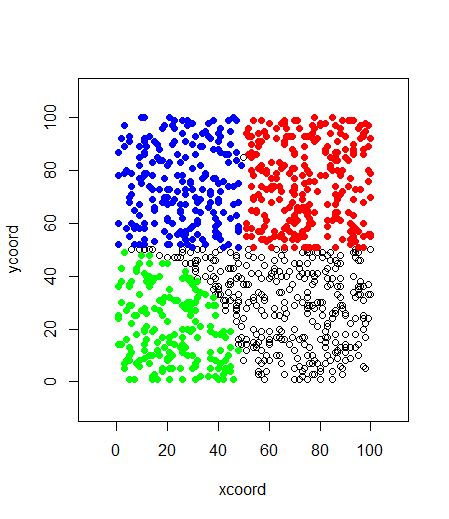
\includegraphics{images/05/01.png}

\begin{itemize}
\tightlist
\item
  1부터 100까지 수 를 랜덤하게 1000개 생성해서 x좌표를 생성하고 xcoord에 저장 하시오 (중복허용)
\item
  1부터 100까지 수 를 랜덤하게 1000개 생성해서 y좌표를 생성하고 ycoord에 저장 하시오 (중복허용)
\item
  x, y 좌표 평면에 xcoord와 ycoord 값을 이용하여 좌표를 (산포도) 그리되 x와 y의 범위가 모두 -10부터 110까지 되도록 지정 하시오 (plot 이용)
\item
  앞서 문제와 같은 plot에 x가 50보다 크고 y가 50보다 큰 곳에 있는 좌표들에 red closed circle로 표현하시오 (which, points, pch parameter 등 이용, 아래 참고)
\end{itemize}

\begin{Shaded}
\begin{Highlighting}[]
\NormalTok{idx }\OtherTok{\textless{}{-}} \FunctionTok{which}\NormalTok{(xcoord}\SpecialCharTok{\textgreater{}}\DecValTok{50} \SpecialCharTok{\&}\NormalTok{ ycoord}\SpecialCharTok{\textgreater{}}\DecValTok{50}\NormalTok{)}
\FunctionTok{points}\NormalTok{(}\AttributeTok{x=}\NormalTok{xcoord[idx], }\AttributeTok{y=}\NormalTok{ycoord[idx], }\AttributeTok{col=}\StringTok{"red"}\NormalTok{, }\AttributeTok{pch=}\DecValTok{19}\NormalTok{)}
\end{Highlighting}
\end{Shaded}

\begin{itemize}
\tightlist
\item
  앞서 문제와 같은 plot에 x가 50보다 작고 y가 50보다 큰 곳에 있는 좌표들에 blue closed circle로 표현하시오 (which, points, pch parameter 등 이용)
\item
  앞서 문제와 같은 plot에 원점으로부터 거리가 50 이하인 좌표들을 green closed circle로 표현 하시오
\end{itemize}

\hypertarget{usuful-functions-ii}{%
\section{Usuful functions II}\label{usuful-functions-ii}}

\begin{Shaded}
\begin{Highlighting}[]
\CommentTok{\#match(), \%in\%, intersect()}

\NormalTok{x }\OtherTok{\textless{}{-}} \DecValTok{1}\SpecialCharTok{:}\DecValTok{10}
\NormalTok{y }\OtherTok{\textless{}{-}} \DecValTok{5}\SpecialCharTok{:}\DecValTok{15}
\FunctionTok{match}\NormalTok{(x, y)}
\NormalTok{x }\SpecialCharTok{\%in\%}\NormalTok{ y}
\FunctionTok{intersect}\NormalTok{(x, y)}

\CommentTok{\#unique()}
\FunctionTok{unique}\NormalTok{(}\FunctionTok{c}\NormalTok{(x, y))}

\CommentTok{\#substr()}
\NormalTok{x }\OtherTok{\textless{}{-}} \StringTok{"Factors, raw vectors, and lists, are converted"}
\FunctionTok{substr}\NormalTok{(x, }\DecValTok{1}\NormalTok{, }\DecValTok{6}\NormalTok{)}

\CommentTok{\#grep()}
\FunctionTok{grep}\NormalTok{(}\StringTok{"raw"}\NormalTok{, x)}

\CommentTok{\#grepl()}
\FunctionTok{grepl}\NormalTok{(}\StringTok{"raw"}\NormalTok{, x)}
\ControlFlowTok{if}\NormalTok{(}\FunctionTok{grepl}\NormalTok{(}\StringTok{"raw"}\NormalTok{, x))\{}
  \FunctionTok{cat}\NormalTok{(}\StringTok{"I found raw!"}\NormalTok{)}
\NormalTok{\}}

\NormalTok{x }\OtherTok{\textless{}{-}} \FunctionTok{paste}\NormalTok{(LETTERS, }\DecValTok{1}\SpecialCharTok{:}\DecValTok{100}\NormalTok{, }\AttributeTok{sep=}\StringTok{""}\NormalTok{)}
\FunctionTok{grep}\NormalTok{(}\StringTok{"A"}\NormalTok{, x)}
\NormalTok{x[}\FunctionTok{grep}\NormalTok{(}\StringTok{"A"}\NormalTok{, x)]}

\FunctionTok{grepl}\NormalTok{(}\StringTok{"A"}\NormalTok{, x)}
\NormalTok{r }\OtherTok{\textless{}{-}} \FunctionTok{grepl}\NormalTok{(}\StringTok{"A"}\NormalTok{, x)}
\ControlFlowTok{if}\NormalTok{(r)\{}
  \FunctionTok{cat}\NormalTok{(}\StringTok{"Yes, I found A"}\NormalTok{)}
\NormalTok{\}}\ControlFlowTok{else}\NormalTok{\{}
  \FunctionTok{cat}\NormalTok{(}\StringTok{"No A"}\NormalTok{)}
\NormalTok{\}}

\CommentTok{\#strsplit()}
\NormalTok{x }\OtherTok{\textless{}{-}} \FunctionTok{c}\NormalTok{(}\StringTok{"Factors, raw vectors, and lists, are converted"}\NormalTok{, }\StringTok{"vectors, or for, strings with"}\NormalTok{)}
\NormalTok{y }\OtherTok{\textless{}{-}} \FunctionTok{strsplit}\NormalTok{(x, }\AttributeTok{split=}\StringTok{", "}\NormalTok{)}

\CommentTok{\#unlist()}
\FunctionTok{unlist}\NormalTok{(y)}

\NormalTok{y }\OtherTok{\textless{}{-}} \FunctionTok{strsplit}\NormalTok{(x, }\AttributeTok{split=}\StringTok{""}\NormalTok{)}
\NormalTok{ychar }\OtherTok{\textless{}{-}} \FunctionTok{unlist}\NormalTok{(y)}
\NormalTok{ycount }\OtherTok{\textless{}{-}} \FunctionTok{table}\NormalTok{(y2)}
\NormalTok{ycount\_sort }\OtherTok{\textless{}{-}} \FunctionTok{sort}\NormalTok{(ycount)}
\NormalTok{ycount\_sort }\OtherTok{\textless{}{-}} \FunctionTok{sort}\NormalTok{(ycount, }\AttributeTok{decreasing =}\NormalTok{ T)}
\NormalTok{ycount\_top }\OtherTok{\textless{}{-}}\NormalTok{ ycount\_sort[}\DecValTok{1}\SpecialCharTok{:}\DecValTok{5}\NormalTok{]}
\NormalTok{ycount\_top\_char }\OtherTok{\textless{}{-}} \FunctionTok{names}\NormalTok{(ycount\_top)}

\CommentTok{\#toupper(), tolower()}
\FunctionTok{toupper}\NormalTok{(ycount\_top\_char)}
\end{Highlighting}
\end{Shaded}

\textbf{Exercises}

built-in 데이터셋 중 \texttt{state.abb} 은 미국의 50개 주에대한 축약어임.

\begin{enumerate}
\def\labelenumi{\arabic{enumi})}
\item
  이 중 문자 A 가 들어가는 주를 뽑아 x에 저장 하시오 (\texttt{grep} 또는 \texttt{grepl} 사용)
\item
  state.abb 중 위 x에 저장된 이름들을 빼고 y에 저장 하시오 (\texttt{match()} 또는 \texttt{\%in\%}사용)
\item
  state.abb에 사용된 알파벳의 갯수를 구하고 가장 많이 쓰인 알파벳을 구하시오 (\texttt{strsplit()}, \texttt{table()} 등 사용)
\end{enumerate}

\textbf{Exercises}

\texttt{iris} 데이터셋의 각 Species 별로 꽃잎과 꽃받침의 길이와 넓이에 대한 평균값들을 구하고 막대그래프를 그리시오

\begin{center}\rule{0.5\linewidth}{0.5pt}\end{center}

이 저작물은 크리에이티브 커먼즈 저작자표시-비영리-변경금지 4.0 국제 라이선스에 따라 이용할 수 있습니다.

\hypertarget{tidyverse}{%
\chapter{tidyverse}\label{tidyverse}}

tidyverse (\url{https://www.tidyverse.org/)는} 데이터 사이언스를 위한 R 기반의 독창적인 패키지들의 모음입니다. Rstudio의 핵심 전문가인 해들리위컴이 (Hadley Wickham) 중심이 되어 만들어 졌으며 기존의 툴보다 쉽고 효율적으로 데이터 분석을 수행할 수 있습니다.

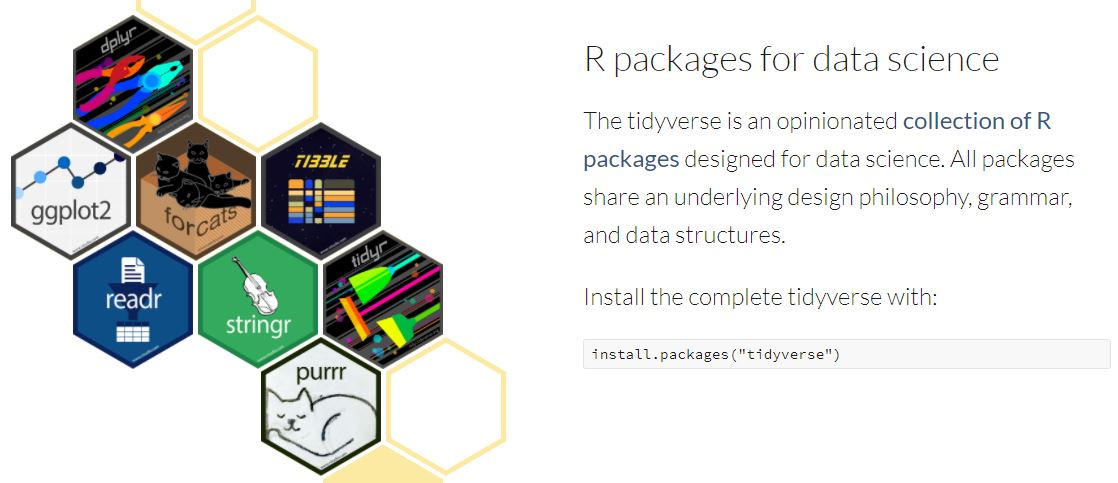
\includegraphics[width=5.72917in,height=\textheight]{images/07/tidyverse.JPG}

데이터사이언스는 넓은 범위의 개념과 방법적인 정도가 있는 것은 아닙니다. 그러나 tidyverse의 목적은 데이터 분석을 위한 핵심이되는 고효율의 툴을 제공하는 것이며 그 철학은 다음과 같은 그림으로 요약할 수 있습니다.

\begin{figure}
\centering
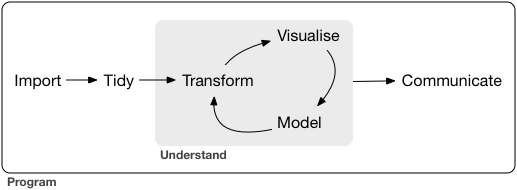
\includegraphics{images/07/data-science.png}
\caption{from \url{https://r4ds.had.co.nz/}}
\end{figure}

\hypertarget{tibble-object-type}{%
\section{tibble object type}\label{tibble-object-type}}

R은 20년 이상된 비교적 오랜 역사를 가진 언어로서 \texttt{data.frame} 형태의 데이터 타입이 가장 많이 사용되고 있습니다. 그러나 당시에는 유용했던 기능이 시간이 흐르면서 몇몇 단점들이 드러나는 문제로 기존 코드를 그대로 유지한채 package 형태로 단점을 보완한 새로운 형태의 tibble 오브젝트 형식을 만들어 냈습니다. 대부분의 R 코드는 여전히 data.frame 형태의 데이터 타입을 사용하고 있으나 tidyverse에서는 \texttt{tibble}이 사용되는 것을 참고하시기 바랍니다.

\begin{Shaded}
\begin{Highlighting}[]
\FunctionTok{library}\NormalTok{(tidyverse)}

\NormalTok{tb }\OtherTok{\textless{}{-}} \FunctionTok{tibble}\NormalTok{(}
  \AttributeTok{x =} \DecValTok{1}\SpecialCharTok{:}\DecValTok{5}\NormalTok{, }
  \AttributeTok{y =} \DecValTok{1}\NormalTok{, }
  \AttributeTok{z =}\NormalTok{ x }\SpecialCharTok{\^{}} \DecValTok{2} \SpecialCharTok{+}\NormalTok{ y}
\NormalTok{)}

\FunctionTok{as\_tibble}\NormalTok{(iris)}
\FunctionTok{head}\NormalTok{(iris)}
\end{Highlighting}
\end{Shaded}

\texttt{tibble}은 \texttt{data.frame}과 다음 몇 가지 점이 다릅니다. \texttt{data.frame}의 경우 타입을 변환할 때 강제로 값의 타입을 바꾸거나 내부 변수의 이름을 바꾸는 경우가 있었으나 \texttt{tibble}은 이를 허용하지 않습니다. 샘플들 (row) 이름을 바꿀수도 없습니다. 또한 프린팅할 때 출력물에 나오는 정보가 다르며 마지막으로 \texttt{data.frame}은 subset에 대한 타입이 바뀔 경우가 있었지만 \texttt{tibble}은 바뀌지 않습니다.

\begin{Shaded}
\begin{Highlighting}[]

\NormalTok{x }\OtherTok{\textless{}{-}} \DecValTok{1}\SpecialCharTok{:}\DecValTok{3}
\NormalTok{y }\OtherTok{\textless{}{-}} \FunctionTok{list}\NormalTok{(}\DecValTok{1}\SpecialCharTok{:}\DecValTok{5}\NormalTok{, }\DecValTok{1}\SpecialCharTok{:}\DecValTok{10}\NormalTok{, }\DecValTok{1}\SpecialCharTok{:}\DecValTok{20}\NormalTok{)}

\FunctionTok{data.frame}\NormalTok{(x, y)}
\FunctionTok{tibble}\NormalTok{(x, y)}
\end{Highlighting}
\end{Shaded}

\texttt{tibble}은 컬럼 하나가 벡터형 변수가 아닌 리스트형 변수가 될 수 있다는 것도 \texttt{data.frame}과 다른 점 입니다.

\begin{Shaded}
\begin{Highlighting}[]
\FunctionTok{names}\NormalTok{(}\FunctionTok{data.frame}\NormalTok{(}\StringTok{\textasciigrave{}}\AttributeTok{crazy name}\StringTok{\textasciigrave{}} \OtherTok{=} \DecValTok{1}\NormalTok{))}
\FunctionTok{names}\NormalTok{(}\FunctionTok{tibble}\NormalTok{(}\StringTok{\textasciigrave{}}\AttributeTok{crazy name}\StringTok{\textasciigrave{}} \OtherTok{=} \DecValTok{1}\NormalTok{))}
\end{Highlighting}
\end{Shaded}

또한 다음과 같이 사용되는 변수의 (\texttt{x}) 참조 범위가 다릅니다.

\begin{Shaded}
\begin{Highlighting}[]

\FunctionTok{data.frame}\NormalTok{(}\AttributeTok{x =} \DecValTok{1}\SpecialCharTok{:}\DecValTok{5}\NormalTok{, }\AttributeTok{y =}\NormalTok{ x }\SpecialCharTok{\^{}} \DecValTok{2}\NormalTok{)}
\FunctionTok{tibble}\NormalTok{(}\AttributeTok{x =} \DecValTok{1}\SpecialCharTok{:}\DecValTok{5}\NormalTok{, }\AttributeTok{y =}\NormalTok{ x }\SpecialCharTok{\^{}} \DecValTok{2}\NormalTok{)}
\end{Highlighting}
\end{Shaded}

\begin{Shaded}
\begin{Highlighting}[]
\NormalTok{df1 }\OtherTok{\textless{}{-}} \FunctionTok{data.frame}\NormalTok{(}\AttributeTok{x =} \DecValTok{1}\SpecialCharTok{:}\DecValTok{3}\NormalTok{, }\AttributeTok{y =} \DecValTok{3}\SpecialCharTok{:}\DecValTok{1}\NormalTok{)}
\FunctionTok{class}\NormalTok{(df1)}
\FunctionTok{class}\NormalTok{(df1[, }\DecValTok{1}\SpecialCharTok{:}\DecValTok{2}\NormalTok{])}
\FunctionTok{class}\NormalTok{(df1[, }\DecValTok{1}\NormalTok{])}

\NormalTok{df2 }\OtherTok{\textless{}{-}} \FunctionTok{tibble}\NormalTok{(}\AttributeTok{x =} \DecValTok{1}\SpecialCharTok{:}\DecValTok{3}\NormalTok{, }\AttributeTok{y =} \DecValTok{3}\SpecialCharTok{:}\DecValTok{1}\NormalTok{)}
\FunctionTok{class}\NormalTok{(df2)}
\FunctionTok{class}\NormalTok{(df2[, }\DecValTok{1}\SpecialCharTok{:}\DecValTok{2}\NormalTok{])}
\FunctionTok{class}\NormalTok{(df2[, }\DecValTok{1}\NormalTok{])}
\FunctionTok{class}\NormalTok{(df2}\SpecialCharTok{$}\NormalTok{x)}
\end{Highlighting}
\end{Shaded}

\hypertarget{tidy-data-structure}{%
\section{Tidy data structure}\label{tidy-data-structure}}

데이터의 변수와 값을 구분하는 일은 적절한 데이터 분석을 위해 필수적인 과정입니다. 특히 복잡하고 사이즈가 큰 데이터일 경우는 더욱 중요할 수 있으나 경험에 의존해서 구분을 하는 것이 대부분 입니다. Tidy data는 이러한 변수와 값의 명확한 구분과 활용을 위한 데이터 구조중 하나 입니다 (Hadley Wickham. Tidy data. \emph{The Journal of Statistical Software}, vol.~59, 2014).

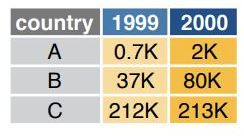
\includegraphics{images/07/notidy.JPG}

tidy data는 다음과 같은 특징이 있습니다.

\begin{itemize}
\tightlist
\item
  각 변수는 해당하는 유일한 하나의 column을 가짐
\item
  각 샘플은 해당하는 유일한 하나의 row를 가짐
\item
  각 관측값은 해당하는 유일한 하나의 cell을 가짐
\end{itemize}

\begin{figure}
\centering
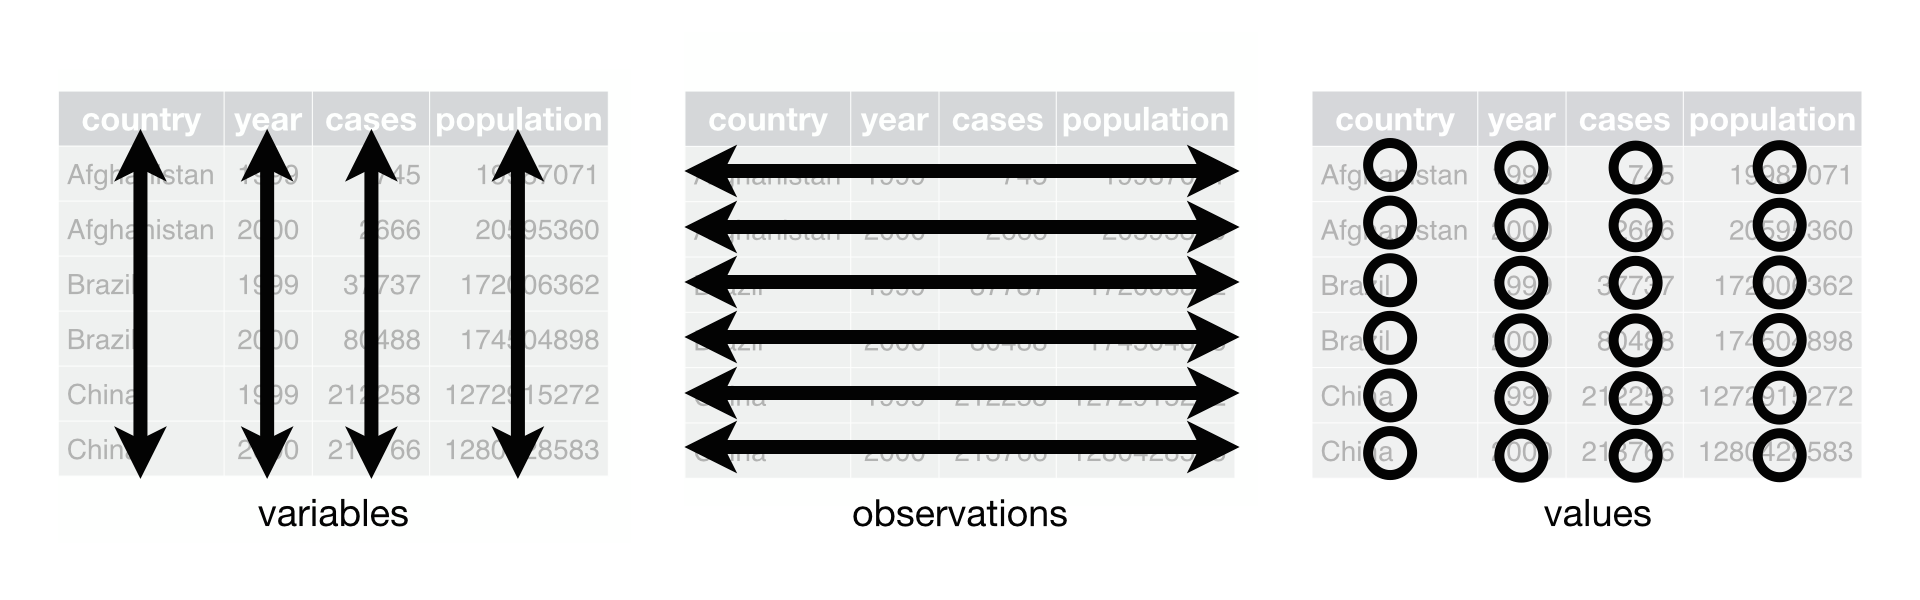
\includegraphics[width=6.25in,height=\textheight]{images/07/tidy-1.png}
\caption{from \url{https://r4ds.had.co.nz/}}
\end{figure}

Tidy 데이터는 Long형 데이터로 알려져 있기도 합니다. 참고로 Wide형 데이터의 경우 샘플 데이터가 늘어날수록 row에 쌓이고 새로운 변수는 column에 쌓이는 방식으로 데이터가 확장되는 형태 입니다. 엑셀에서 볼 수 있는 일반적인 형식으로 다음 그림과 같습니다.

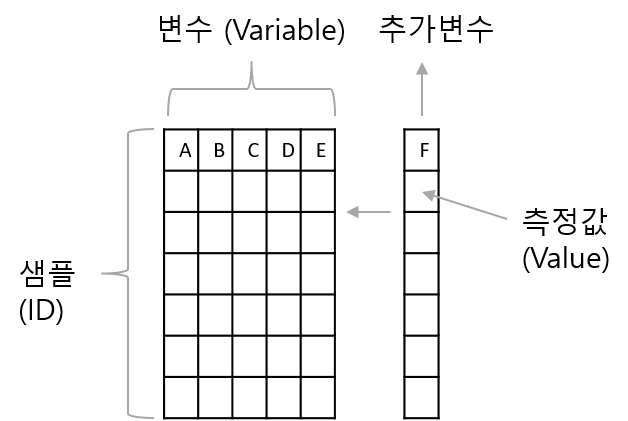
\includegraphics{images/07/05.png}

Long형 데이터의 경우 ID, variable, value 세가지 변수만 기억하면 되겠습니다. 위 wide형 데이터 경우를 보면 ID, variable, 그리고 value 이 세가지 요인이 주요 구성 요소임을 알 수 있습니다. Long형으로 변환할 경우 샘플을 참조할 수 있는 어떤 변수 (variable)도 ID가 될 수 있으며 2개 이상의 변수가 ID로 지정될 수 있습니다. 참고로 ID를 지정할 경우 해당 ID는 가능하면 중복되지 않는 값들을 갖는 변수를 사용해야 식별자로서 기능을 적절히 수행할 수 있습니다. Long형을 사용할 경우 데이터의 변수가 늘어나도 행의 수만 늘어나므로 코딩의 일관성과 변수들의 그룹을 만들어서 분석하는 등의 장점이 있습니다. 아래는 새로운 변수 F가 추가될 때 long 형 데이터에 데이터가 추가되는 경우를 나타낸 그림 입니다.

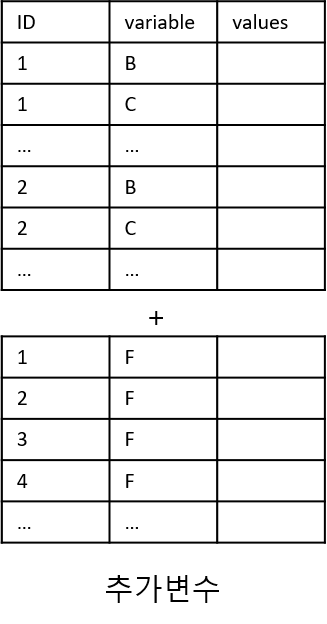
\includegraphics{images/07/06.png}

\hypertarget{pivoting}{%
\section{Pivoting}\label{pivoting}}

일반적으로 얻어지는 데이터의 형태는 wide형이며 이를 Long형으로 변환하기 위해서는 \texttt{tidyverse} 패키지에 속한 \texttt{tidyr} 패키지의 \texttt{pivot\_longer}와 \texttt{pivot\_wider}를 사용합니다. 또한 \texttt{reshape2} 패키지의 \texttt{melt}함수와 그 반대의 경우 \texttt{dcast} 함수를 사용할 수도 있습니다. 본 강의에서는 \texttt{tidyr} 패키지를 사용합니다. wide형 데이터를 long형으로 변환하거나 long형을 wide형으로 변환하는 작업을 pivoting 이라고 합니다.

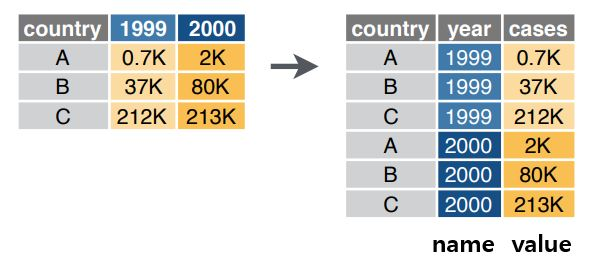
\includegraphics{images/07/wide2long.JPG}

\texttt{airquality} 데이터는 전형적인 wide형 데이터로 특정 날짜에 네 개의 변수에 해당하는 값들을 측정했습니다. 이 데이터를 long형으로 바꿀 경우 ID를 날짜로 하면 데이터들을 식별 할 수 있습니다. 그런데 날짜는 변수가 Month와 Day두 개로 나누어져 있으므로 다음과 같이 두 변수를 식별 변수로 (ID로) 사용 합니다. 확인을 위해 상위 5개의 데이터만 가지고 형 변환을 진행해 보겠습니다.

\begin{Shaded}
\begin{Highlighting}[]
\NormalTok{airquality}

\NormalTok{myair }\OtherTok{\textless{}{-}}\NormalTok{ airquality[}\DecValTok{1}\SpecialCharTok{:}\DecValTok{5}\NormalTok{,]}
\NormalTok{myair\_long }\OtherTok{\textless{}{-}} \FunctionTok{pivot\_longer}\NormalTok{(myair, }\FunctionTok{c}\NormalTok{(}\StringTok{"Ozone"}\NormalTok{, }\StringTok{"Solar.R"}\NormalTok{, }\StringTok{"Wind"}\NormalTok{, }\StringTok{"Temp"}\NormalTok{))}
\NormalTok{myair\_long }
\NormalTok{myair\_long2 }\OtherTok{\textless{}{-}} \FunctionTok{pivot\_longer}\NormalTok{(myair, }\FunctionTok{c}\NormalTok{(Ozone, Solar.R, Wind, Temp))}
\NormalTok{myair\_long2 }
\NormalTok{myair\_long3 }\OtherTok{\textless{}{-}} \FunctionTok{pivot\_longer}\NormalTok{(myair, }\SpecialCharTok{!}\FunctionTok{c}\NormalTok{(Month, Day))}
\NormalTok{myair\_long3}
\end{Highlighting}
\end{Shaded}

생성되는 long형 데이터의 변수 이름인 name과 value는 다음 파라메터를 지정하여 바꿀 수 있습니다.

\begin{Shaded}
\begin{Highlighting}[]

\NormalTok{myair\_long }\OtherTok{\textless{}{-}} \FunctionTok{pivot\_longer}\NormalTok{(myair, }
                          \FunctionTok{c}\NormalTok{(Ozone, Solar.R, Wind, Temp), }
                          \AttributeTok{names\_to =} \StringTok{"Type"}\NormalTok{, }
                          \AttributeTok{values\_to =} \StringTok{"Observation"}\NormalTok{)}
\NormalTok{myair\_long }
\end{Highlighting}
\end{Shaded}

long형 데이터를 wide형 데이터로 변환 할 수도 있습니다.

\begin{Shaded}
\begin{Highlighting}[]
\FunctionTok{pivot\_wider}\NormalTok{(myair\_long, }\AttributeTok{names\_from =}\NormalTok{ Type, }\AttributeTok{values\_from =}\NormalTok{ Observation)}
\end{Highlighting}
\end{Shaded}

\textbf{Exercises}

\begin{enumerate}
\def\labelenumi{\arabic{enumi})}
\tightlist
\item
  다음 데이터가 long형인지 wide형인지 판단하시오\\
\item
  long형이면 wide형으로 wide형이면 long형으로 변환하시오
\end{enumerate}

\begin{Shaded}
\begin{Highlighting}[]
\NormalTok{stocks }\OtherTok{\textless{}{-}} \FunctionTok{tibble}\NormalTok{(}
  \AttributeTok{year   =} \FunctionTok{c}\NormalTok{(}\DecValTok{2015}\NormalTok{, }\DecValTok{2015}\NormalTok{, }\DecValTok{2016}\NormalTok{, }\DecValTok{2016}\NormalTok{),}
  \AttributeTok{month  =} \FunctionTok{c}\NormalTok{(   }\DecValTok{1}\NormalTok{,    }\DecValTok{2}\NormalTok{,     }\DecValTok{1}\NormalTok{,    }\DecValTok{2}\NormalTok{),}
  \AttributeTok{profit =} \FunctionTok{c}\NormalTok{(}\FloatTok{1.88}\NormalTok{, }\FloatTok{0.59}\NormalTok{, }\FloatTok{0.92}\NormalTok{, }\FloatTok{0.17}\NormalTok{)}
\NormalTok{)}
\end{Highlighting}
\end{Shaded}

\texttt{ggplot}을 이용한 그래프 작성에는 위와 같은 long형 데이터가 주로 사용됩니다. R을 이용한 데이터 가시화는 \texttt{dplyr} 패키지로 wide형 데이터를 편집하고 \texttt{pivot\_longer} 함수로 long형 데이터로 변환 후 \texttt{ggplot}을 이용하는 방식으로 수행합니다. 두 데이터 포멧에 대한 좀 더 구체적인 내용은 다음 링크를 참고하시기 바랍니다. \url{https://www.theanalysisfactor.com/wide-and-long-data/}

\hypertarget{separating-and-uniting}{%
\section{Separating and uniting}\label{separating-and-uniting}}

데이터를 분석할 때 하나의 컬럼에 두 개 이상의 변수값이 저장되어 있거나 두 개의 변수를 하나의 컬럼으로 합해야 하는 경우가 종종 있습니다. 전자의 경우 \texttt{separate()} 함수를 사용해서 두 변수(컬럼)으로 나누어 줄 수 있으며 후자의 경우 \texttt{unite()} 함수를 사용하여 두 변수를 하나의 값으로 병합할 수 있습니다. 다음은 \texttt{airquality}데이터에서 Month와 Day 변수를 하나의 컬럼으로 병합하여 Date라는 변수로 만들어 주는 경우의 예 입니다.

\begin{Shaded}
\begin{Highlighting}[]
\NormalTok{newairquality }\OtherTok{\textless{}{-}} \FunctionTok{unite}\NormalTok{(airquality, Date, Month, Day, }\AttributeTok{sep=}\StringTok{"."}\NormalTok{)}
\NormalTok{newairquality}
\end{Highlighting}
\end{Shaded}

\texttt{separate()}함수를 사용하면 다음과 같이 해당 변수의 값을 나누어 다시 두 개의 변수(컬럼)으로 나누어 줄 수 있습니다.

\begin{Shaded}
\begin{Highlighting}[]

\FunctionTok{separate}\NormalTok{(newairquality, }\AttributeTok{col=}\NormalTok{Date, }\AttributeTok{into =} \FunctionTok{c}\NormalTok{(}\StringTok{"Month"}\NormalTok{, }\StringTok{"Day"}\NormalTok{), }\AttributeTok{sep =} \StringTok{"}\SpecialCharTok{\textbackslash{}\textbackslash{}}\StringTok{."}\NormalTok{)}
\end{Highlighting}
\end{Shaded}

\hypertarget{dplyr-and-pipe-operator}{%
\section{dplyr and pipe operator}\label{dplyr-and-pipe-operator}}

\texttt{dplyr} (\url{https://dplyr.tidyverse.org/}) 은 \texttt{ggplot2}을 개발한 해들리위컴이 (Hadley Wickham) 중심이 되어 만들어 졌으며 \texttt{ggplot2}와 함께 \texttt{tidyverse}의 (\url{https://www.tidyverse.org/}) 핵심 패키지 입니다. \texttt{dplyr}은 데이터를 다루는 크기나 분석의 속도, 편의성을 향상시켜 새롭게 만들어놓은 패키지 입니다. 기존 \texttt{apply}와 같은 행렬 연산 기능과 \texttt{subset}, \texttt{split}, \texttt{group} 와 같은 행렬 편집 기능을 더하여 만들어진 도구라고 할 수 있습니다.

\texttt{dplyr}의 전신이라 할 수 있는 \texttt{plyr} 패키지는 다음과 같이 설명이 되어 있습니다. \emph{A set of tools for a common set of problems: you need to split up a big data structure into homogeneous pieces, apply a function to each piece and then combine all the results back together.} 즉 split-apply-combine 세 가지 동작을 쉽게 할 수 있도록 만들어 놓은 툴 입니다. R이 다른 언어에 비해 데이터 분석에서 주목을 받는 이유로 \texttt{split}, \texttt{apply} 등의 행렬 연산 함수가 발달한 것을 내세우는데 \texttt{dplyr}은 이들을 보다 더 편리하게 사용할 수 있도록 만들어 놓은 것 입니다.

\texttt{dplyr}의 사용을 위해서는 여러 명령을 연속적으로 수행하도록 해주는 \texttt{\%\textgreater{}\%} 파이프 오퍼레이터의 이해가 필요합니다. 파이프 오퍼레이터의 작동법은 간단히 \texttt{\%\textgreater{}\%}의 왼쪽 코드의 결과를 출력으로 받아 오른쪽 코드의 입력 (첫번째 파라미터의 값)으로 받아들이는 작동을 합니다 (\textbf{단축키: Shift+Ctrl+m}). 다음 예에서 보면 \texttt{sin(pi)} 와 같은 함수의 일반적인 사용법 대신 \texttt{pi\ \%\textgreater{}\%\ sin} 처럼 사용해도 똑같은 결과를 보여줍니다. \texttt{cos(sin(pi))}와 같이 여러 합수를 중첩하여 사용할 경우와 비교해서 코드의 가독성이나 효율 측면에서 크게 향상된 방법을 제공해 줍니다.

\begin{Shaded}
\begin{Highlighting}[]
\FunctionTok{library}\NormalTok{(dplyr)}

\NormalTok{pi }\SpecialCharTok{\%\textgreater{}\%}\NormalTok{ sin}
\FunctionTok{sin}\NormalTok{(pi)}
\NormalTok{pi }\SpecialCharTok{\%\textgreater{}\%}\NormalTok{ sin }\SpecialCharTok{\%\textgreater{}\%}\NormalTok{ cos}
\FunctionTok{cos}\NormalTok{(}\FunctionTok{sin}\NormalTok{(pi))}
\end{Highlighting}
\end{Shaded}

특히 \texttt{\%\textgreater{}\%}는 이후 설명할 \texttt{dplyr}의 \texttt{group\_by}, \texttt{split}, \texttt{filter}, \texttt{summary} 등의 행렬 편집/연산 함수를 빈번히 다양한 조합으로 쓰게되는 상황에서 더 큰 효과를 발휘할 수 있습니다.

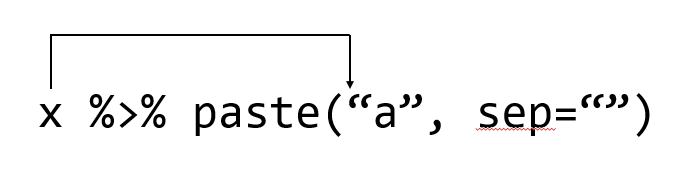
\includegraphics[width=5.20833in,height=\textheight]{images/07/02.PNG}

pipe operator의 왼쪽 구문의 결과가 오른쪽 구문의 첫 번째 파라미터의 입력 값으로 처리된다고 말씀 드렸습니다. 즉, 함수에서 사용되는 파라미터가 여러개일 경우가 있으므로 기본적으로 \texttt{\%\textgreater{}\%} 의 왼쪽 구문의 출력 값은 오른쪽 구문 (함수)의 첫 번째 인자의 입력값으로 들어가는 것 입니다. 이는 다음 예들을 통해서 명확히 알 수 있습니다. 먼저 \texttt{paste}함수는 그 파라미터로 \texttt{,}로 구분되는 여러개의 입력 값을 가질 수 있습니다. 따라서 다음 코드는 \texttt{x}가 \texttt{paste}의 첫 번째 파라미터로 들어가게 되어 \texttt{"1a",\ "2a",\ "3a",\ "4a",\ "5a"}로 a 앞에 x 값들이 붙어서 출력된 것을 알 수 있습니다.

\begin{Shaded}
\begin{Highlighting}[]
\NormalTok{x }\OtherTok{\textless{}{-}} \DecValTok{1}\SpecialCharTok{:}\DecValTok{5}
\NormalTok{x }\SpecialCharTok{\%\textgreater{}\%} \FunctionTok{paste}\NormalTok{(}\StringTok{"a"}\NormalTok{, }\AttributeTok{sep=}\StringTok{""}\NormalTok{)}
\end{Highlighting}
\end{Shaded}

특정 데이터셋의 컬럼별 평균을 구하고 각 평균의 합을 구할 경우를 생각해 봅시다. R에서는 \texttt{colMeans}라는 특별한 함수를 제공하여 컬럼별로 평균을 계산해 줍니다. 그 후 sum 함수를 사용하여 최종 원하는 값을 얻을 수 있습니다. 이러한 코드를 \texttt{\%\textgreater{}\%} 오퍼레이터를 사용한 경우의 코드와 비교해 볼 수 있습니다.

\begin{Shaded}
\begin{Highlighting}[]
\NormalTok{x }\OtherTok{\textless{}{-}} \FunctionTok{data.frame}\NormalTok{(}\AttributeTok{x=}\FunctionTok{c}\NormalTok{(}\DecValTok{1}\SpecialCharTok{:}\DecValTok{100}\NormalTok{), }\AttributeTok{y=}\FunctionTok{c}\NormalTok{(}\DecValTok{201}\SpecialCharTok{:}\DecValTok{300}\NormalTok{))}
\FunctionTok{sum}\NormalTok{(}\FunctionTok{colMeans}\NormalTok{(x))}

\NormalTok{x }\OtherTok{\textless{}{-}} \FunctionTok{data.frame}\NormalTok{(}\AttributeTok{x=}\FunctionTok{c}\NormalTok{(}\DecValTok{1}\SpecialCharTok{:}\DecValTok{100}\NormalTok{), }\AttributeTok{y=}\FunctionTok{c}\NormalTok{(}\DecValTok{201}\SpecialCharTok{:}\DecValTok{300}\NormalTok{))}
\NormalTok{x }\SpecialCharTok{\%\textgreater{}\%}\NormalTok{ colMeans }\SpecialCharTok{\%\textgreater{}\%}\NormalTok{ sum}
\end{Highlighting}
\end{Shaded}

그럼 만약 두 번째 파라미터에 입력으로 왼쪽 구문의 출력을 받아들이고 싶을 경우는 place holer \texttt{.} 을 사용하면 되겠습니다. \texttt{round} 함수는 두 개의 파라미터를 설정할 있 이으며 digits 라는 두 번째 파라미터에 값을 pipe operator로 넘겨주고 싶을 경우 아래와 같이 표현할 수 있습니다.

\begin{Shaded}
\begin{Highlighting}[]
\DecValTok{6} \SpecialCharTok{\%\textgreater{}\%} \FunctionTok{round}\NormalTok{(pi, }\AttributeTok{digits=}\NormalTok{.)}
\FunctionTok{round}\NormalTok{(pi, }\AttributeTok{digits=}\DecValTok{6}\NormalTok{)}
\end{Highlighting}
\end{Shaded}

\textbf{Exercises}

\begin{enumerate}
\def\labelenumi{\arabic{enumi})}
\tightlist
\item
  pipe operator를 사용해서 \texttt{airquality}데이터를 long형으로 전환하는 코드를 작성하시오 (단 col 파라메터에는 Ozone, Solar.R, Wind, Temp 변수를 넣음)\\
\item
  pipe operator를 사용해서 \texttt{airquality}데이터의 Month와 Day 변수(컬럼)을 Date 변수로 병합하는 코드를 작성하시오
\end{enumerate}

\hypertarget{dplyr---important-functions}{%
\section{dplyr - Important functions}\label{dplyr---important-functions}}

이제 \texttt{dplyr} 패키지에서 제공하는 함수를 사용해 보겠습니다. \texttt{dplyr}을 구성하는 중요한 함수는 다음과 같습니다.

\begin{itemize}
\tightlist
\item
  \texttt{filter()} - 샘플 (rows) 선택
\item
  \texttt{arrange()} - 샘플들의 정렬 순서 변경
\item
  \texttt{select()} - 변수 (columns) 선택
\item
  \texttt{mutate()} - 새로운 변수 만들기
\item
  \texttt{summarise()} - 대표값 만들기
\item
  \texttt{group\_by()} - 그룹별로 계산 수행
\item
  \texttt{join()} - 두 tibble 또는 data.frame을 병합할 때 사용
\end{itemize}

이 함수들은 \texttt{\%\textgreater{}\%}와 함께 쓰이면서 강력한 성능을 발휘합니다. \texttt{summarise} 함수는 특정 값들의 통계 값을 계산해 주는 함수이며 그 외 함수들은 행렬 편집을 위한 함수들로 보시면 되겠습니다. 간단한 예제를 수행하면서 각각의 기능을 살펴보고 왜 \texttt{dplyr}이 널리 사용되고 그 장점이 무엇인지 파악해 보도록 하겠습니다.

\texttt{iris} 데이터는 세 종류의 iris 품종에 대한 꽃잎과 꽃받침의 length와 with를 측정해 놓은 데이터 입니다. \texttt{head}와 \texttt{str} 명령어를 \texttt{\%\textgreater{}\%}를 이용해서 데이터를 살펴 봅니다.

\begin{Shaded}
\begin{Highlighting}[]
\FunctionTok{library}\NormalTok{(tidyverse)}

\NormalTok{iris }\SpecialCharTok{\%\textgreater{}\%} \FunctionTok{head}\NormalTok{(}\DecValTok{10}\NormalTok{)}
\NormalTok{iris }\SpecialCharTok{\%\textgreater{}\%}\NormalTok{ str}
\end{Highlighting}
\end{Shaded}

\hypertarget{filter}{%
\subsection{filter}\label{filter}}

먼저 아래와 같이 \texttt{filter} 함수를 사용해서 원하는 조건의 데이터 (샘플)을 골라낼 수 있습니다.

\begin{Shaded}
\begin{Highlighting}[]
\FunctionTok{library}\NormalTok{(dplyr)}

\FunctionTok{head}\NormalTok{(iris)}
\NormalTok{iris }\SpecialCharTok{\%\textgreater{}\%} \FunctionTok{filter}\NormalTok{(Species}\SpecialCharTok{==}\StringTok{"setosa"}\NormalTok{)}
\NormalTok{iris }\SpecialCharTok{\%\textgreater{}\%} \FunctionTok{filter}\NormalTok{(Species}\SpecialCharTok{==}\StringTok{"setosa"} \SpecialCharTok{|}\NormalTok{ Species}\SpecialCharTok{==}\StringTok{"versicolor"}\NormalTok{)}
\NormalTok{iris }\SpecialCharTok{\%\textgreater{}\%} \FunctionTok{filter}\NormalTok{(Species}\SpecialCharTok{==}\StringTok{"setosa"} \SpecialCharTok{\&}\NormalTok{ Species}\SpecialCharTok{==}\StringTok{"versicolor"}\NormalTok{)}
\NormalTok{iris }\SpecialCharTok{\%\textgreater{}\%} 
  \FunctionTok{filter}\NormalTok{(Species}\SpecialCharTok{==}\StringTok{"setosa"} \SpecialCharTok{|}\NormalTok{ Species}\SpecialCharTok{==}\StringTok{"versicolor"}\NormalTok{) }\SpecialCharTok{\%\textgreater{}\%} 
\NormalTok{  dim}
\end{Highlighting}
\end{Shaded}

\texttt{filter}의 \texttt{,}로 구분되는 매개변수는 \texttt{and} 로직으로 묶인 조건입니다. 지난 강좌에서 보셨듯 R에서 \texttt{and}는 \texttt{\&}, \texttt{or}는 \texttt{\textbar{}}, 그리고 not은 \texttt{!} 으로 사용하면 되며 \texttt{filter}에서 \texttt{,}로 구분된 조건은 \texttt{and}와 같다고 보시면 되겠습니다.

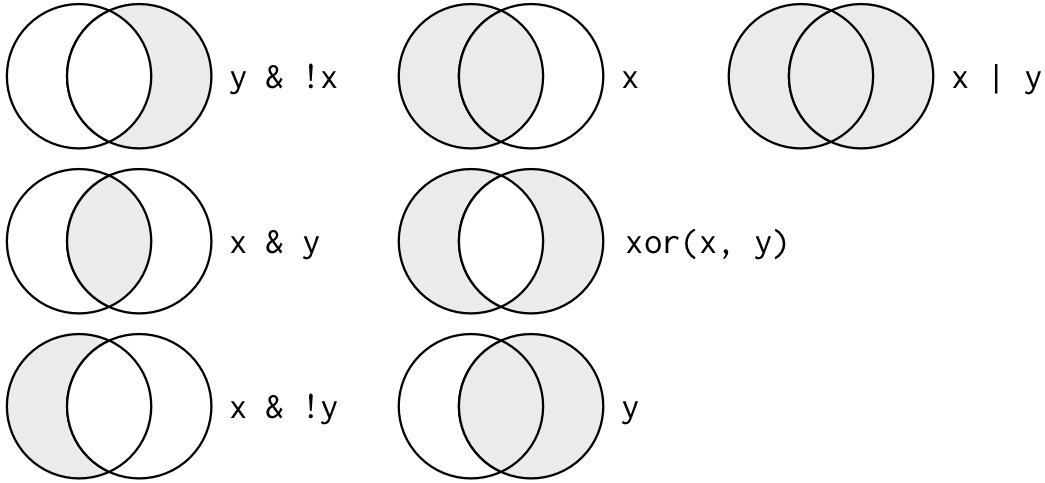
\includegraphics[width=5.20833in,height=\textheight]{images/07/03.png}

Image from (\url{https://r4ds.had.co.nz/})

\hypertarget{arrange}{%
\subsection{arrange}\label{arrange}}

\texttt{arrange()}는 지정된 변수를 기준으로 값의 크기순서로 샘플들의 배열 순서 즉, row의 순서를 바꾸는 기능을 수행합니다. 기본으로 크기가 커지는 순서로 정렬이 진행되며 작아지는 순서를 원할 경우 \texttt{desc} 함수를 사용할 수 있습니다.

\begin{Shaded}
\begin{Highlighting}[]
\NormalTok{iris }\SpecialCharTok{\%\textgreater{}\%} \FunctionTok{arrange}\NormalTok{(Sepal.Length)}
\NormalTok{iris }\SpecialCharTok{\%\textgreater{}\%} \FunctionTok{arrange}\NormalTok{(}\FunctionTok{desc}\NormalTok{(Sepal.Length))}
\NormalTok{iris }\SpecialCharTok{\%\textgreater{}\%} \FunctionTok{arrange}\NormalTok{(Sepal.Length, Sepal.Width)}
\end{Highlighting}
\end{Shaded}

\hypertarget{select}{%
\subsection{select}\label{select}}

\texttt{select()} 는 주어진 데이터셋으로부터 관심있는 변수를 (column) 선택하여 보여줍니다. 다음 helper 함수들은 select 함수와 같이 유용하게 쓰일 수 있습니다.

\begin{quote}
starts\_with(``abc'') - ``abc'' 로 시작하는 문자열을 갖는 변수 이름
ends\_with(``xyz'') - ``xyz''으로 끝나는 문자열을 갖는 변수 이름
contains(``ijk'') - ``ijk'' 문자열을 포함하는 변수 이름
matches(``(.)\textbackslash1'') - 정규식, 반복되는 문자
\end{quote}

\begin{Shaded}
\begin{Highlighting}[]
\FunctionTok{head}\NormalTok{(iris)}
\NormalTok{iris }\SpecialCharTok{\%\textgreater{}\%} \FunctionTok{select}\NormalTok{(Species, }\FunctionTok{everything}\NormalTok{()) }\SpecialCharTok{\%\textgreater{}\%} \FunctionTok{head}\NormalTok{(}\DecValTok{5}\NormalTok{)}
\NormalTok{iris }\SpecialCharTok{\%\textgreater{}\%} \FunctionTok{select}\NormalTok{(Species, }\FunctionTok{everything}\NormalTok{())}
\NormalTok{iris }\SpecialCharTok{\%\textgreater{}\%} \FunctionTok{select}\NormalTok{(}\SpecialCharTok{{-}}\NormalTok{Species)}
\NormalTok{iris }\SpecialCharTok{\%\textgreater{}\%} \FunctionTok{select}\NormalTok{(}\FunctionTok{starts\_with}\NormalTok{(}\StringTok{\textquotesingle{}S\textquotesingle{}}\NormalTok{))}
\NormalTok{iris }\SpecialCharTok{\%\textgreater{}\%} \FunctionTok{select}\NormalTok{(}\AttributeTok{obs =} \FunctionTok{starts\_with}\NormalTok{(}\StringTok{\textquotesingle{}S\textquotesingle{}}\NormalTok{))}
\end{Highlighting}
\end{Shaded}

아래는 \texttt{matches} 함수를 사용한 방법 입니다. 좀 더 복잡한 패턴을 적용하여 변수들을 선택할 수 있으며 \texttt{grep} 함수를 사용할 경우도 정규식 패턴을 적용할 수 있습니다.

\begin{Shaded}
\begin{Highlighting}[]
\NormalTok{iris2 }\OtherTok{\textless{}{-}} \FunctionTok{rename}\NormalTok{(iris, }\AttributeTok{aavar =}\NormalTok{ Petal.Length)}
\FunctionTok{select}\NormalTok{(iris2, }\FunctionTok{matches}\NormalTok{(}\StringTok{"(.)}\SpecialCharTok{\textbackslash{}\textbackslash{}}\StringTok{1"}\NormalTok{))}
\NormalTok{tmp }\OtherTok{\textless{}{-}}\NormalTok{iris[,}\DecValTok{3}\SpecialCharTok{:}\DecValTok{5}\NormalTok{]}
\FunctionTok{colnames}\NormalTok{(iris)[}\FunctionTok{grep}\NormalTok{(}\StringTok{"\^{}S"}\NormalTok{, }\FunctionTok{colnames}\NormalTok{(iris))]}
\NormalTok{iris[,}\FunctionTok{grep}\NormalTok{(}\StringTok{"\^{}S"}\NormalTok{, }\FunctionTok{colnames}\NormalTok{(iris))]}
\NormalTok{tmp}
\end{Highlighting}
\end{Shaded}

아래 \texttt{(.)\textbackslash{}\textbackslash{}1}은 하나의 문자 \texttt{.}가 (어떤 문자든) 한 번 더 \texttt{\textbackslash{}\textbackslash{}1} 사용된 변수 이름을 말하며 이는 \texttt{aavar} 의 \texttt{aa}밖에 없으므로 \texttt{aavar}가 선택됩니다. \texttt{grep}에서 \texttt{\^{}} 표시는 맨 처음을 나타내므로 \texttt{\^{}S}는 S로 시작하는 문자가 되겠습니다. 따라서 \texttt{grep("\^{}S",\ colnames(iris))}의 경우 컬럼 이름 중 S로 시작하는 이름은 True로 그렇지 않으면 False 값을 리턴합니다.

\hypertarget{mutate}{%
\subsection{mutate}\label{mutate}}

\texttt{mutate()} 함수는 새로운 변수를 추가할 수 있는 기능을 제공하며 앞에서 배웠던 \texttt{within()}과 비슷하다고 볼 수 있습니다. 아래와 같이 \texttt{mutate}함수는 sepal\_ratio라는 변수를 새로 만들어서 기존 iris 데이터들과 함께 반환해 줍니다.

\begin{Shaded}
\begin{Highlighting}[]
\NormalTok{iris2 }\OtherTok{\textless{}{-}}\NormalTok{ iris }\SpecialCharTok{\%\textgreater{}\%} \FunctionTok{mutate}\NormalTok{(}\AttributeTok{sepal\_ratio =}\NormalTok{ Sepal.Length}\SpecialCharTok{/}\NormalTok{Sepal.Width)}
\FunctionTok{head}\NormalTok{(iris2)}
\end{Highlighting}
\end{Shaded}

\hypertarget{summarise}{%
\subsection{summarise}\label{summarise}}

\texttt{summarise()}는 \texttt{data.frame}내 특정 변수의 값들로 하나의 요약값/대푯값을 만들어 줍니다. \texttt{summarise} 함수는 단독으로 쓰이기 보다는 \texttt{group\_by()} 기능과 병행해서 쓰이는 경우에 유용하게 쓰입니다. \texttt{summarise\_all()} 함수를 사용하면 모든 변수에 대해서 지정된 함수를 실행합니다.

\begin{Shaded}
\begin{Highlighting}[]
\NormalTok{iris }\SpecialCharTok{\%\textgreater{}\%} \FunctionTok{summarise}\NormalTok{(}\FunctionTok{mean}\NormalTok{(Sepal.Length), }\AttributeTok{m=}\FunctionTok{mean}\NormalTok{(Sepal.Width))}
\NormalTok{iris }\SpecialCharTok{\%\textgreater{}\%} 
  \FunctionTok{group\_by}\NormalTok{(Species) }\SpecialCharTok{\%\textgreater{}\%} 
  \FunctionTok{summarise}\NormalTok{(}\FunctionTok{mean}\NormalTok{(Sepal.Width))}

\NormalTok{iris }\SpecialCharTok{\%\textgreater{}\%} 
  \FunctionTok{group\_by}\NormalTok{(Species) }\SpecialCharTok{\%\textgreater{}\%} 
  \FunctionTok{summarise\_all}\NormalTok{(mean)}

\NormalTok{iris }\SpecialCharTok{\%\textgreater{}\%} 
  \FunctionTok{group\_by}\NormalTok{(Species) }\SpecialCharTok{\%\textgreater{}\%} 
  \FunctionTok{summarise}\NormalTok{(}\FunctionTok{across}\NormalTok{(}\FunctionTok{everything}\NormalTok{(), mean))}


\NormalTok{iris }\SpecialCharTok{\%\textgreater{}\%} 
  \FunctionTok{group\_by}\NormalTok{(Species) }\SpecialCharTok{\%\textgreater{}\%} 
  \FunctionTok{summarise\_all}\NormalTok{(sd)}

\NormalTok{iris }\SpecialCharTok{\%\textgreater{}\%} 
  \FunctionTok{group\_by}\NormalTok{(Species) }\SpecialCharTok{\%\textgreater{}\%} 
  \FunctionTok{summarise}\NormalTok{(}\FunctionTok{across}\NormalTok{(}\FunctionTok{everything}\NormalTok{(), sd))}
\end{Highlighting}
\end{Shaded}

\hypertarget{join}{%
\subsection{join}\label{join}}

\texttt{join} 함수는 데이터를 병합해주는 기능을 수행하는 함수 입니다. 네 가지 종류의 함수가 있으며 (\texttt{left\_join()}, 'right\_join()\texttt{,\ \textquotesingle{}inner\_join()}, 'full\_join()\texttt{)\ 기본적으로\ 공통되는\ 이름의\ 변수를\ (key)\ 이용해서\ 공통되는\ 샘플끼리\ 자동으로\ 병합해\ 주는\ 기능을\ 수행합니다.}by`에서 지정해준 파라메터의 값을 기준으로 기능이 수행 됩니다.

\begin{Shaded}
\begin{Highlighting}[]
\NormalTok{df1 }\OtherTok{\textless{}{-}} \FunctionTok{data.frame}\NormalTok{(}\AttributeTok{id=}\FunctionTok{c}\NormalTok{(}\DecValTok{1}\NormalTok{,}\DecValTok{2}\NormalTok{,}\DecValTok{3}\NormalTok{,}\DecValTok{4}\NormalTok{,}\DecValTok{5}\NormalTok{,}\DecValTok{6}\NormalTok{), }\AttributeTok{age=}\FunctionTok{c}\NormalTok{(}\DecValTok{30}\NormalTok{, }\DecValTok{41}\NormalTok{, }\DecValTok{33}\NormalTok{, }\DecValTok{56}\NormalTok{, }\DecValTok{20}\NormalTok{, }\DecValTok{17}\NormalTok{))}
\NormalTok{df2 }\OtherTok{\textless{}{-}} \FunctionTok{data.frame}\NormalTok{(}\AttributeTok{id=}\FunctionTok{c}\NormalTok{(}\DecValTok{4}\NormalTok{,}\DecValTok{5}\NormalTok{,}\DecValTok{6}\NormalTok{,}\DecValTok{7}\NormalTok{,}\DecValTok{8}\NormalTok{,}\DecValTok{9}\NormalTok{), }\AttributeTok{gender=}\FunctionTok{c}\NormalTok{(}\StringTok{"f"}\NormalTok{, }\StringTok{"f"}\NormalTok{, }\StringTok{"m"}\NormalTok{, }\StringTok{"m"}\NormalTok{, }\StringTok{"f"}\NormalTok{, }\StringTok{"m"}\NormalTok{))}

\FunctionTok{inner\_join}\NormalTok{(df1, df2, }\AttributeTok{by=}\StringTok{"id"}\NormalTok{)}
\FunctionTok{left\_join}\NormalTok{(df1, df2, }\StringTok{"id"}\NormalTok{)}
\FunctionTok{right\_join}\NormalTok{(df1, df2, }\StringTok{"id"}\NormalTok{)}
\FunctionTok{full\_join}\NormalTok{(df1, df2, }\StringTok{"id"}\NormalTok{)}

\CommentTok{\# vs.}
\FunctionTok{cbind}\NormalTok{(df1, df2)}
\end{Highlighting}
\end{Shaded}

\hypertarget{code-comparison}{%
\section{Code comparison}\label{code-comparison}}

이제 \texttt{split}, \texttt{apply}, \texttt{combine}을 활용하여 평균을 구하는 코드와 \texttt{dplyr} 패키지를 사용하여 만든 코드를 비교해 보도록 하겠습니다. iris 데이터를 분석하여 품종별로 꽃받침의 길이 (Sepal.length)의 평균과 표준편차, 그리고 샘플의 수를 구해보는 코드입니다.

\texttt{split}은 \texttt{factor}형 변수인 Species를 기준으로 \texttt{iris} 데이터를 나누어 주는 역할을 하며 \texttt{lapply}는 \texttt{list} 형 데이터인 \texttt{iris\_split}을 각 리스트의 각각의 원소들에 대해서 임의의 함수 \texttt{function(x)...} 를 수행하는 역할을 합니다. 마지막 \texttt{data.frame}으로 최종 경로를 combine 합니다.

\begin{Shaded}
\begin{Highlighting}[]
\NormalTok{iris\_split }\OtherTok{\textless{}{-}} \FunctionTok{split}\NormalTok{(iris, iris}\SpecialCharTok{$}\NormalTok{Species)}
\NormalTok{iris\_means }\OtherTok{\textless{}{-}} \FunctionTok{lapply}\NormalTok{(iris\_split, }\ControlFlowTok{function}\NormalTok{(x)\{}\FunctionTok{mean}\NormalTok{(x}\SpecialCharTok{$}\NormalTok{Sepal.Length)\})}
\NormalTok{iris\_sd }\OtherTok{\textless{}{-}} \FunctionTok{lapply}\NormalTok{(iris\_split, }\ControlFlowTok{function}\NormalTok{(x)\{}\FunctionTok{sd}\NormalTok{(x}\SpecialCharTok{$}\NormalTok{Sepal.Length)\})}
\NormalTok{iris\_cnt }\OtherTok{\textless{}{-}} \FunctionTok{lapply}\NormalTok{(iris\_split, }\ControlFlowTok{function}\NormalTok{(x)\{}\FunctionTok{length}\NormalTok{(x}\SpecialCharTok{$}\NormalTok{Sepal.Length)\})}
\NormalTok{iris\_df }\OtherTok{\textless{}{-}} \FunctionTok{data.frame}\NormalTok{(}\FunctionTok{unlist}\NormalTok{(iris\_cnt), }\FunctionTok{unlist}\NormalTok{(iris\_means), }\FunctionTok{unlist}\NormalTok{(iris\_sd))}
\end{Highlighting}
\end{Shaded}

아래는 \texttt{dplyr} 패키지를 사용한 코드 입니다.

\begin{Shaded}
\begin{Highlighting}[]
\NormalTok{iris\_df }\OtherTok{\textless{}{-}}\NormalTok{ iris }\SpecialCharTok{\%\textgreater{}\%} 
  \FunctionTok{group\_by}\NormalTok{(Species) }\SpecialCharTok{\%\textgreater{}\%} 
  \FunctionTok{summarise}\NormalTok{(}\AttributeTok{n=}\FunctionTok{n}\NormalTok{(), }\AttributeTok{mean=}\FunctionTok{mean}\NormalTok{(Sepal.Length), }\AttributeTok{sd=}\FunctionTok{sd}\NormalTok{(Sepal.Length))}
\end{Highlighting}
\end{Shaded}

위에서 보듯 \texttt{dplyr} 패키지를 사용할 경우 그 결과는 같으나 코드의 가독성과 효율성면에서 장점을 보여줍니다. \texttt{iris} 데이터를 받아서 Species에 명시된 그룹으로 나누고 원하는 함수를 타깃 컬럼에 대해서 적용하라는 의미 입니다. 다음은 모든 변수에 대한 평균을 구하는 코드 입니다.

\begin{Shaded}
\begin{Highlighting}[]
\NormalTok{iris\_mean\_df }\OtherTok{\textless{}{-}}\NormalTok{ iris }\SpecialCharTok{\%\textgreater{}\%} 
  \FunctionTok{group\_by}\NormalTok{(Species) }\SpecialCharTok{\%\textgreater{}\%} 
  \FunctionTok{summarise}\NormalTok{(}\FunctionTok{across}\NormalTok{(}\FunctionTok{everything}\NormalTok{(), mean))}
\end{Highlighting}
\end{Shaded}

자세한 ggplot의 내용은 다음시간에 학습하겠지만 각 평균에 대한 막대그래프를 그러보겠습니다.

\begin{Shaded}
\begin{Highlighting}[]
\FunctionTok{library}\NormalTok{(ggplot2)}

\NormalTok{iris\_mean\_df2 }\OtherTok{\textless{}{-}}\NormalTok{ iris\_mean\_df }\SpecialCharTok{\%\textgreater{}\%} 
  \FunctionTok{pivot\_longer}\NormalTok{(}\SpecialCharTok{{-}}\NormalTok{Species)}

\FunctionTok{ggplot}\NormalTok{(iris\_mean\_df2, }\FunctionTok{aes}\NormalTok{(}\AttributeTok{x=}\NormalTok{Species, }\AttributeTok{y=}\NormalTok{value, }\AttributeTok{fill=}\NormalTok{name)) }\SpecialCharTok{+}
  \FunctionTok{geom\_bar}\NormalTok{(}\AttributeTok{stat=}\StringTok{"identity"}\NormalTok{, }\AttributeTok{position=}\StringTok{"dodge"}\NormalTok{)}
\end{Highlighting}
\end{Shaded}

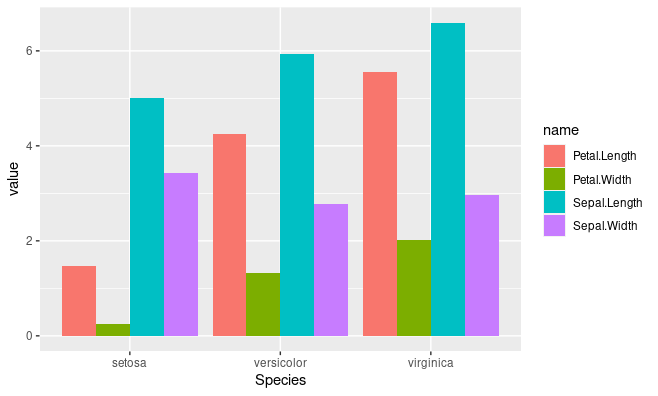
\includegraphics[width=5.20833in,height=\textheight]{images/08/Rplot01.png}

\textbf{Exercises}

InsectSprays 데이터는 살충제 6종에 대한 살충력을 (죽은 벌래의 마릿수) 나타내는 데이터이다. 각 살충제별로 평균과 표준편차를 구하시오

\textbf{Exercises}

dplyr 패키지의 starwars 는 스타워즈 영화에 나오는 등장인물들을 분석한 데이터셋 이다. 종족에 따른 키의 평균과 표준편차를 구하시오. (NA 데이터는 제외하고 분석)

\textbf{Exercises}

airquality 데이터는 뉴욕주의 몇몇 지점에서의 공기질을 측정한 데이터이다. 데이터에서 NA를 제거하고 각 월별로 평균 오존, 자외선, 풍속, 및 온도에 대한 평균과 표준편차를 구하시오

\begin{Shaded}
\begin{Highlighting}[]

\NormalTok{airmean }\OtherTok{\textless{}{-}}\NormalTok{ airquality }\SpecialCharTok{\%\textgreater{}\%} 
  \FunctionTok{filter}\NormalTok{(}\FunctionTok{complete.cases}\NormalTok{(.)) }\SpecialCharTok{\%\textgreater{}\%} 
  \FunctionTok{select}\NormalTok{(}\SpecialCharTok{{-}}\NormalTok{Day) }\SpecialCharTok{\%\textgreater{}\%} 
  \FunctionTok{group\_by}\NormalTok{(Month) }\SpecialCharTok{\%\textgreater{}\%} 
  \FunctionTok{summarise}\NormalTok{(}\FunctionTok{across}\NormalTok{(}\FunctionTok{everything}\NormalTok{(), mean)) }\SpecialCharTok{\%\textgreater{}\%} 
  \FunctionTok{pivot\_longer}\NormalTok{(}\SpecialCharTok{{-}}\NormalTok{Month, }\AttributeTok{values\_to =} \StringTok{"mean"}\NormalTok{)}

\NormalTok{airsd }\OtherTok{\textless{}{-}}\NormalTok{ airquality }\SpecialCharTok{\%\textgreater{}\%} 
  \FunctionTok{filter}\NormalTok{(}\FunctionTok{complete.cases}\NormalTok{(.)) }\SpecialCharTok{\%\textgreater{}\%} 
  \FunctionTok{select}\NormalTok{(}\SpecialCharTok{{-}}\NormalTok{Day) }\SpecialCharTok{\%\textgreater{}\%} 
  \FunctionTok{group\_by}\NormalTok{(Month) }\SpecialCharTok{\%\textgreater{}\%} 
  \FunctionTok{summarise}\NormalTok{(}\FunctionTok{across}\NormalTok{(}\FunctionTok{everything}\NormalTok{(), sd)) }\SpecialCharTok{\%\textgreater{}\%} 
  \FunctionTok{pivot\_longer}\NormalTok{(}\SpecialCharTok{{-}}\NormalTok{Month, }\AttributeTok{values\_to =} \StringTok{"sd"}\NormalTok{)}
\end{Highlighting}
\end{Shaded}

참고로 errorbar가 있는 막대그래프를 그려보겠습니다. 이를 위해서 먼저 두 테이블을 병합한 후 \texttt{ggplot2} 패키지의 \texttt{ggplot} 함수를 이용해서 그래프를 그립니다. 자세한 \texttt{ggplot}의 내용은 다음시간에 학습하겠습니다.

\begin{Shaded}
\begin{Highlighting}[]

\NormalTok{airdata }\OtherTok{\textless{}{-}} \FunctionTok{left\_join}\NormalTok{(airmean, airsd, }\AttributeTok{by=}\FunctionTok{c}\NormalTok{(}\StringTok{"Month"}\NormalTok{, }\StringTok{"name"}\NormalTok{))}

\FunctionTok{ggplot}\NormalTok{(airdata, }\FunctionTok{aes}\NormalTok{(}\AttributeTok{x=}\NormalTok{Month, }\AttributeTok{y=}\NormalTok{mean, }\AttributeTok{fill=}\NormalTok{name)) }\SpecialCharTok{+}
  \FunctionTok{geom\_bar}\NormalTok{(}\AttributeTok{stat=}\StringTok{"identity"}\NormalTok{, }\AttributeTok{position=}\StringTok{"dodge"}\NormalTok{) }\SpecialCharTok{+}
  \FunctionTok{geom\_errorbar}\NormalTok{(}\FunctionTok{aes}\NormalTok{(}\AttributeTok{ymin=}\NormalTok{mean}\SpecialCharTok{{-}}\NormalTok{sd, }\AttributeTok{ymax=}\NormalTok{mean}\SpecialCharTok{+}\NormalTok{sd), }\AttributeTok{position=}\FunctionTok{position\_dodge}\NormalTok{(}\AttributeTok{width=}\FloatTok{0.9}\NormalTok{), }\AttributeTok{width=}\FloatTok{0.4}\NormalTok{)}
\end{Highlighting}
\end{Shaded}

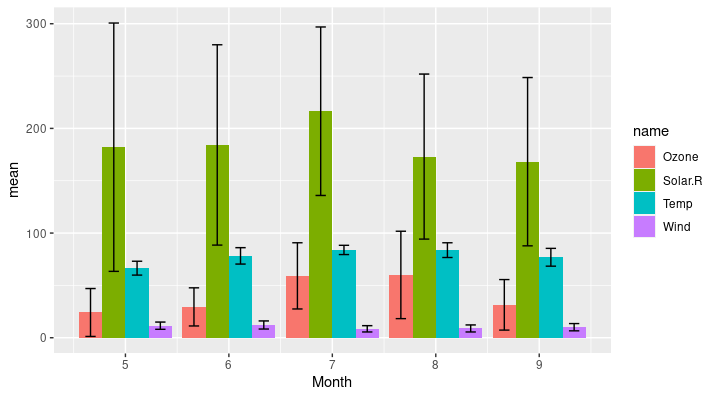
\includegraphics[width=5.20833in,height=\textheight]{images/08/Rplot02.png}

\begin{center}\rule{0.5\linewidth}{0.5pt}\end{center}

이 저작물은 크리에이티브 커먼즈 저작자표시-비영리-변경금지 4.0 국제 라이선스에 따라 이용할 수 있습니다.

  \bibliography{book.bib,packages.bib}

\end{document}
